\documentclass{book}
\usepackage{graphicx} % Required for inserting images

\usepackage{mathtools}
\usepackage{listings, xcolor}
\usepackage{color}
\usepackage{geometry}
\usepackage{graphicx}
\usepackage{tikz-qtree}
\usetikzlibrary{arrows}
\usepackage{multirow}
\usepackage{hyperref}

\usepackage{amsmath}
\usepackage{amsfonts}
\usepackage[makeroom]{cancel}

\usepackage{algorithm}
\usepackage[noend]{algpseudocode}
\makeatletter
\def\BState{\State\hskip-\ALG@thistlm}
\makeatother


\newgeometry{
left=   1 in,
bottom= 1.5 in,
right=  1 in,
top=    1 in
}


\title{Advanced Algorithms Notes}
\author{Riccardo Cappi}
\date{February 2024}

\begin{document}

\maketitle

\section{Disclaimer}
These are just my notes that I used to prepare for the exam. So, probably, there will be both spelling and conceptual errors. Feel free to contact me at riccardo.cappi@studenti.unipd.it if you find any errors. This is the github repo where you can find the latex files of the notes: \url{https://github.com/riccardocappi/Computer-Science-notes}

\tableofcontents


\chapter{Lec 01 - Graph Algorithms I}

\section{Graphs: The basis}
A graph is a representation of the relationships between \textbf{pairs} of objects. We denote a graph as follows:
\[G = (V, E)\]
where $V$ is a \textbf{set} of vertices (nodes) and $E$ is a collection of edges. An edge is a pair of vertices $(u, v)$ which indicates the connection between the two nodes.
\begin{itemize}
    \item if $(u, v) = (v, u)$ the graph is \textbf{undirected}
    \item if $(u, v) \neq (v, u)$ the graph is \textbf{directed}
\end{itemize}
In directed graphs an edge is usually called \textit{"arc"}.

Examples of real-world graphs are:
\begin{itemize}
    \item Road networks: $(Cities, Roads)$
    \item Computer networks (e.g. internet): $(Computers, connections)$
    \item World Wide Web: $(Web pages, hyperlinks)$
    \item Social networks: $(People, friendship \,\, connections)$
\end{itemize}

\section{Terminology}
\begin{itemize}
    \item Given an edge $e = (u, v)$, $e$ is \textbf{incident} on $u$ and $v$, while $u, v$ are \textbf{adjacent}.

    \item The \textbf{neighbors} of a vertex $u$ are all the vertices $v$ such that $(u, v) \in E$. 

    \item The \textbf{degree} of a vertex $d(v)$ is the number of edges incident on $v$.
\end{itemize}

\section{Concepts}
\begin{itemize}
    \item \textbf{Simple path}: A sequence of nodes $v_{1}, v_{2}, ..., v_{k}$ all distinct such that $(v_{i}, v_{i + 1}) \in E \,\, \forall 1 \leq i < k$. Having all distinct nodes makes the path a simple path. 

    \item \textbf{Cycle}: is a path such that $v_{1} = v_{k}$

    \item \textbf{Sub-graph:} $G' = (V', E')$ such that $V' \subseteq V, \,\, E' \subseteq E$ and the edges of $E'$ are incident only on $V'$.

    \item \textbf{Spanning sub-graph:} a sub-graph with $V' = V$

    \item \textbf{Connected graph:} a graph is connected if $\forall u, v \in V$ it exists a path from $u$ to $v$.

    \item \textbf{Connected components:} a partition of $G$ in sub-graphs $G_{i} = (V_{i}, E_{i})$ such that $\forall 1 \leq i < k$ 
    \begin{itemize}
        \item $G_{i}$ is connected.
        \item $V$ = $V_{1} \cup V_{2} \cup ... \cup V_{k}$
        \item $E = E_{1} \cup E_{2} \cup... \cup E_{k}$
        \item $\forall i \neq j$ there is no edge between $V_{i}$ and $V_{j}$
    \end{itemize}
    If $G$ is connected, then $k = 1$.

    \item \textbf{Tree:} connected graph without cycles.

    \item \textbf{Forest:} set of trees (disjoint)

    \item \textbf{Spanning tree:} a spanning connected sub-graph without cycles (it exists only if $G$ is connected).

    \item \textbf{Spanning forest:} a spanning sub-graph without cycles.
\end{itemize}

\section{Basic problems}
\begin{itemize}
    \item Traversal
    \item Connectivity (tell if the graph is connected or not)
    \item Compute connected components
    \item Minimum-weight spanning trees
    \item Shortest paths
    \item ...
\end{itemize}

\section{Notations and Properties}
\begin{itemize}
    \item $n = |V|$
    \item $m = |E|$
    \item The \textbf{size} of the graph is given by $n + m$
    \item $\sum_{v \in V}d(v) = 2m$ because in the summation every edge counts twice.
    \item $m \leq \binom{n}{2}$
    \item if $G$ is a tree $m = n - 1$ because, fixed a root, $E$ represents father-child similarities, which are $n - 1$.
    \item if $G$ is connected $m \geq n - 1$ because $G$ is a \textit{"tree"} that may have cycles, thus it can only have more edges.
    \item if $G$ is acyclic $m \leq n - 1$ because $G$ is a tree that may not be connected, thus it can only have less edges.
\end{itemize}


\chapter{Lec 02 - Problem Solving Agent}
\section{Solving Problems by Searching}
We'll describe one kind of \textbf{goal-based} agent called a problem-solving agent. Our discussion of problem solving begins with precise definitions of \textbf{problems} and their \textbf{solutions} and give several examples to illustrate these definitions. We then describe several
general-purpose search algorithms that can be used to solve these problems. We will see several \textbf{uninformed} search algorithms, algorithms that are given no information about the problem other than its definition. Let's start with an example:\newline\newline
Imagine an agent in the city of Arad, Romania, enjoying a touring holiday. Now, suppose the agent has a nonrefundable ticket to fly out of Bucharest the following day. In that case, it makes sense for the agent to adopt the \textbf{goal} of getting to Bucharest by driving across various cities. Therefore, the \textbf{problem formulation} can be defined as follows:
\begin{itemize}
    \item Formulate goal: be in Bucharest
    \item Formulate problems:
    \begin{itemize}
        \item states: various cities
        \item actions: drive between cities
    \end{itemize}
    \item Solution: sequence of cities; e.g. Arad, Sibiu, Fagaras, Bucharest
\end{itemize}
\begin{center}
    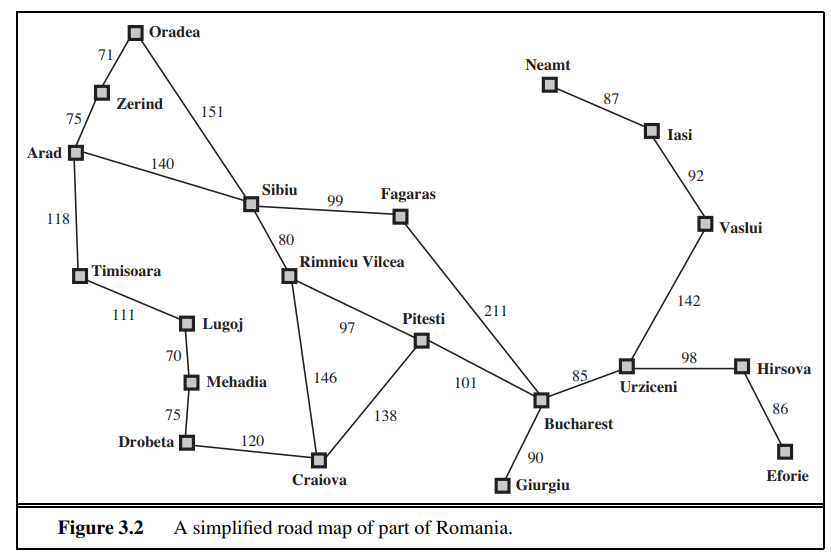
\includegraphics[scale=0.8]{images/Romania.png}
\end{center}
We assume that the environment is \textbf{observable}, so the agent always knows the current state. For the agent driving in Romania, it’s reasonable to suppose that each city on the map has a sign indicating its presence to arriving drivers. We also assume the environment is \textbf{discrete}, so at any given state there are only finitely many actions to choose from. This is true for navigating in Romania because each city is connected to a small number of other cities. We will assume the environment is \textbf{known}, so the agent knows which states are reached by each action. (Having an accurate map suffices to meet this condition for navigation problems.) Finally, we assume that the environment is \textbf{deterministic}, so each action has exactly one outcome.\newline\newline
The process of looking for a sequence of actions that reaches the goal is called \textbf{search}. A search algorithm takes a problem as input and returns a \textbf{solution} in the form of an action sequence.
\begin{center}
    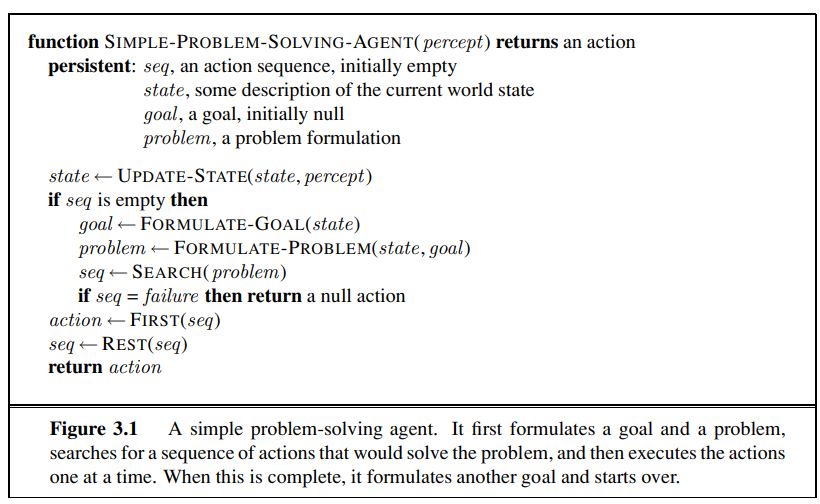
\includegraphics[scale=0.8]{images/problem-solving agent.png}
\end{center}
A problem can be defined formally by four components:
\begin{itemize}
    \item The \textbf{initial state} that the agent starts in. For example, the initial state for our agent in Romania might be described as \textit{In(Arad)}.

    \item A description of what each action does; the formal name for this is the \textbf{transition model}. We also use the term \textbf{successor} to refer to any state reachable from a given state by a single action. This can be described by a set $E(x)$ of action-state pairs, e.g. $E(In(Arad)) = \{<Arad \rightarrow Zerind, Zerind>, ...\}$. An alternative formulation for the successor function can be the actions that can be performed in a given state.

    \item The \textbf{goal test}, which determines whether a given state is a goal state. The goal can be explicit, e.g. the singleton set \footnote{There can be multiple goal states} $\{In(Bucharest)\}$, or implicit, an abstract property rather than an explicitly enumerated set of states.

    \item A \textbf{path cost} function that assigns a numeric cost to each path. The problem-solving agent chooses a cost function that reflects its own performance measure. For the agent trying to get to Bucharest, time is of the essence, so the cost of a path might be its length in kilometers. The \textbf{step cost} of taking action $a$ in state $s$ to reach state $s'$ is denoted by $c(s, a, s')$, assumed to be $\geq 0$.
\end{itemize}
The preceding elements define a problem and can be gathered into a single data structure that is given as input to a problem-solving algorithm. A solution to a problem is an action sequence that leads from the initial state to a goal state. Solution quality is measured by the path cost function, and an \textbf{optimal solution} has the lowest path cost among all solutions.

\section{Selecting a State Space}
Real world is absurdly complex. Compare the simple state description we have chosen, $In(Arad)$, to an actual crosscountry trip, where the state of the world includes so many things: the traveling companions, the current radio program, the scenery out of the window, the proximity of law enforcement officers, etc. All these considerations are left out of our state descriptions because they are irrelevant to the problem of finding a route to Bucharest. The process of removing detail from a representation is called \textbf{abstraction}.
\newline\newline
In addition to abstracting the state description, we must abstract the actions themselves.\newline\newline
Now consider a solution to the abstract problem: for example, the path from Arad to Sibiu to Rimnicu Vilcea to Pitesti to Bucharest. This abstract solution corresponds to a large number of more detailed paths.
\newline\newline
The choice of a good abstraction thus involves removing as much detail as possible while retaining validity and ensuring that the abstract actions are easy to carry out.

\section{Searching for Solutions}
A solution is an action sequence, so search algorithms work by considering various possible action sequences. The possible action sequences starting at the initial state form a \textbf{search tree} with the initial state at the root; the branches are actions and the \textbf{nodes} correspond to states in the \textbf{state space} of the problem.
\begin{center}
    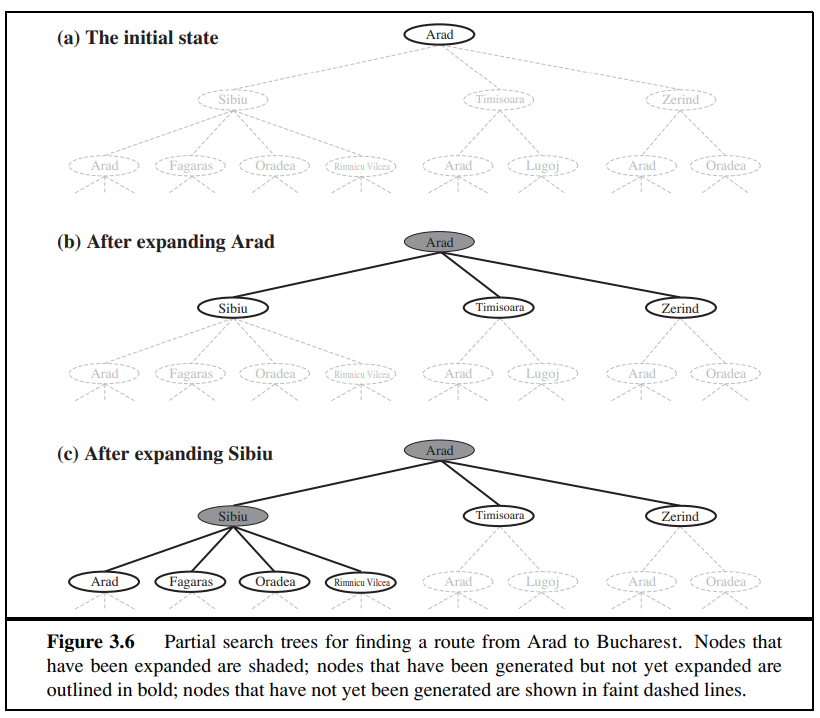
\includegraphics[scale=0.8]{images/search tree.png}
\end{center}
We start from the root and, at each step, we need to check whether we reached the goal state. Then, we need to consider taking various actions. We do this by \textbf{expanding} the current state, that is, applying each legal action to the current state, thereby \textbf{generating} a new set of states. In the case of the figure above, we add three branches from the parent node $In(Arad)$ leading to three new child nodes: $In(Sibiu)$, $In(Timisoara)$, and $In(Zerind)$. Now we must choose which of these three possibilities to consider further.\newline\newline
This is the essence of search, following up one option now and putting the others aside for later. The set of all leaf nodes available for expansion at any given point is called the \textbf{frontier}. The process of expanding nodes on the frontier continues until either a solution is found or there are no more states to expand.
\begin{center}
    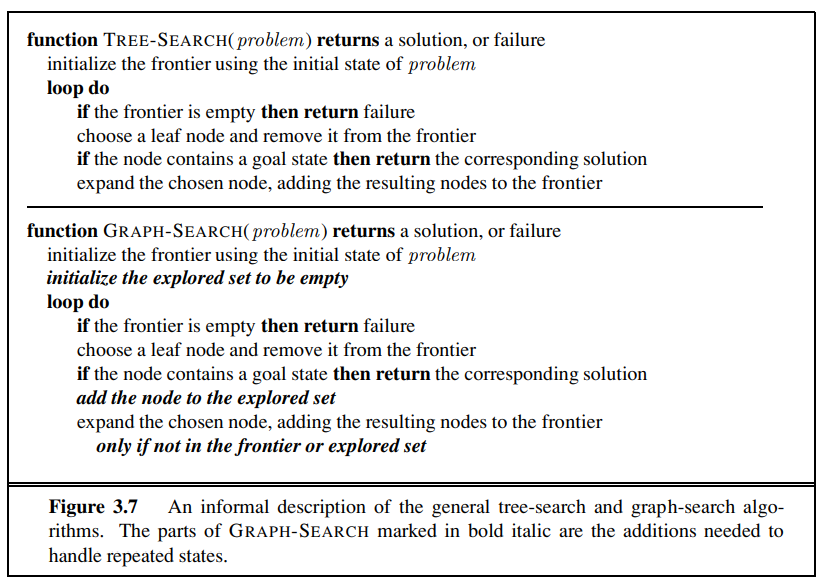
\includegraphics[scale=0.8]{images/tree search2.png}
\end{center}
Search algorithms all share the basic structure above; they vary primarily according to how they choose which state to expand next, the so-called search strategy.\newline\newline
In the figure representing the search tree of the \textit{driving through Romania} problem we can notice that it includes the path from Arad to Sibiu and back to Arad again. We say that $In(Arad)$ is a \textbf{repeated state} in the search tree, generated in this case by a \textbf{loopy path}.\newline\newline
The way to avoid exploring redundant paths is to remember where one has been. To do this, we augment the TREE-SEARCH algorithm with a data structure called the \textbf{explored set} (also known as the closed list), which remembers every expanded node. Newly generated nodes
that match previously generated nodes can be discarded instead of being added to the frontier. This new algorithm is called GRAPH-SEARCH.\newline\newline
Clearly, the search tree constructed by the GRAPH-SEARCH algorithm contains at most one copy of each state, so we can think of it as growing a tree directly on the state-space graph. Furthermore, the frontier \textbf{separates} the state-space graph into the explored region and the unexplored region, so that every path from the initial state to an unexplored state has to pass through a state in the frontier.\newline\newline
Up to now, we have not been very careful to distinguish between nodes and states, but in writing detailed algorithms it’s important to make that distinction. A node is a bookkeeping data structure used to represent the search tree. It includes \textit{parent, children, depth, path cost}. A state corresponds to a configuration of the
world. Thus, nodes are on particular paths whereas states are not. Furthermore, two different nodes can contain the same world state if that state is generated via two different search paths.\newline\newline
Now that we have nodes, we need somewhere to put them. The frontier needs to be stored in such a way that the search algorithm can easily choose the next node to expand according to its preferred strategy. The appropriate data structure for this is a \textbf{queue}.

\section{Uninformed Search Strategies}
Uniformed Search Strategies include the following:
\begin{itemize}
    \item \textbf{Breadth-first search:} Breadth-first search is a simple strategy in which the root node is expanded first, then all the successors of the root node are expanded next, then their successors, and so on. In general, all the nodes are expanded at a given depth in the search tree before any nodes at the next level are expanded. The frontier is implemented using a FIFO queue.

    \item \textbf{Uniform-cost search:} The idea is to expand least-cost unexpanded node. This is done by storing the frontier as a priority queue ordered by path cost.

    \item \textbf{Depth-first search:} Depth-first search always expands the deepest node in the current frontier of the search tree. the frontier is implemented as a LIFO queue.

    \item \textbf{Iterative deepening depth-first search:} Iterative deepening search (or iterative deepening depth-first search) which repeatedly applies depth first search limiting the depth of the tree. It does this by gradually increasing the limit, first 0, then 1, then 2, and so on, until a goal is found.

    \item \textbf{Bidirectional search:} The idea behind bidirectional search is to run two simultaneous searches—one forward from the initial state and the other backward from the goal—hoping that the two searches meet in the middle.

\end{itemize}
We can evaluate an algorithm’s performance in four ways:
\begin{itemize}
    \item \textbf{Completeness:} Is the algorithm guaranteed to find a solution when there is one?

    \item \textbf{Optimality:} Does the strategy find the optimal solution in terms of cost?

    \item \textbf{Time complexity:} How long does it take to find a solution?

    \item \textbf{Space complexity:} How much memory is needed to perform the search?
\end{itemize}
The evaluation of the previously presented strategies is the following:
\begin{center}
    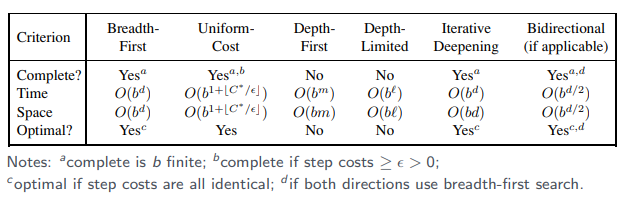
\includegraphics[]{images/evaluation.png}
\end{center}
where:
\begin{itemize}
    \item $b$ is the branching factor (how many successor a node has)

    \item $d$ is the depth of the shallowest solution

    \item $m$ is the maximum depth of the search tree

    \item $l$ is the depth limit
\end{itemize}
We can easily see that \textbf{Breadth-first search} is complete; if the shallowest goal node is at some finite depth $d$, breadth-first search will eventually find it after generating all shallower nodes. Note that as soon as a goal node is generated, we know it is the shallowest goal node because all shallower nodes must have been generated already
and failed the goal test. However, the shallowest goal node is not necessarily the optimal one. Furthermore, every node generated remains in
memory, making the space complexity $O(b^d)$\newline\newline
On the other hand, \textbf{Uniform-cost search} is optimal in general. First, we observe that whenever uniform-cost search selects a node $n$ for expansion, the optimal path to that node has been found. Then,
because step costs are non-negative, paths never get shorter as nodes are added.\newline\newline
The properties of \textbf{depth-first search} depend strongly on whether the graph-search or tree-search version is used. The graph-search version, which avoids repeated states and redundant paths, is complete in finite state spaces because it will eventually expand every node. The tree-search version, on the other hand, is not complete (it may get stuck in a loop). The time complexity of depth-first tree search is $O(b^m)$. Note that $m$ itself can be much larger than $d$. So far, depth-first search seems to have no clear advantage over breadth-first search, so why do we include it? The reason is the space complexity. For a graph search, there is no advantage, but a depth-first tree search needs to store only a single path from the root to a leaf node, along with the remaining unexpanded sibling nodes for each node on the
path. Once a node has been expanded, it can be removed from memory as soon as all its descendants have been fully explored.\newline\newline
We can combine the completeness of BFS and the space saving of DFS with the \textbf{Iterative deepening search}. This strategy may seem wasteful because states are generated multiple times. It turns out this is not too costly. The reason is that in a search tree with the same (or nearly the same) branching factor at each level, most of the nodes are in the bottom level, so it does not matter much that the upper levels are generated multiple times.\newline\newline



\chapter{Lec 03 - From DFS to BFS}

\section{More applications of DFS}
DFS can also be used to solve the following 2 problems:
\begin{itemize}
    \item Connected Components: Labelling all the vertices of $G$ such that 2 vertices have the same label iff they are in the same connected components.
    \item Connectivity: Return whether the graph is connected or not. 
\end{itemize}

\subsection{Connected Components}
\begin{algorithm}
\caption{ConnectedComponents}\label{Conn.Comp.}
    \begin{algorithmic}[1]
    \Procedure{ConnectedComp ($G$)}{}
        \For{$v \gets 1$ to $n$}
            \State $L_{V}[v].ID = 0$
        \EndFor
        \State $k \gets 0$
        \For{$v \gets 1$ to $n$}
            \If{$L_{V}[v].ID = 0$}
                \State $k \gets k + 1$
                \State DFS($G, v, k$)
            \EndIf
        \EndFor
    \EndProcedure
    \end{algorithmic}
\end{algorithm}
We have to modify the DFS algorithm in such a way that $L_{V}[v] \gets k$. The $ID$ field of each node is no more either 0 or 1, but it corresponds to the ID of the $k$-th connected component. 

\subsection{Connectivity}
\begin{algorithm}
\caption{Connectivity}\label{Connectivity}
    \begin{algorithmic}[1]
    \Procedure{Connectivity ($G$)}{}
        \For{$v \gets 1$ to $n$}
            \State $L_{V}[v].ID = 0$
        \EndFor
        \State $k \gets 0$
        \For{$v \gets 1$ to $n$}
            \If{$L_{V}[v].ID = 0$}
                \State $k \gets k + 1$
                \State DFS($G, v, k$)
            \EndIf
        \EndFor
        \State \textbf{if} $k = 1$ \textbf{return} $Yes$ \textbf{else} $False$
    \EndProcedure
    \end{algorithmic}
\end{algorithm}
The algorithm is similar to the one used for computing the connected components, but in this case we return if the graph is connected or not ($k = 1$).\newline\newline
The complexity of both algorithms is $\Theta(n + m)$.

\section{Summary}
Given a graph $G = (V, E)$, the following problems can be solved using DFS:
\begin{itemize}
    \item Test if $G$ is connected.
    \item Find the connected components of $G$.
    \item Find a spanning tree of $G$ (if $G$ is connected).
    \item Find a path between 2 vertices (if any).
    \item Find a cycle (if any).
\end{itemize}

\section{Breadth-First search (BFS)}
BFS is an \textbf{iterative} algorithm that, starting from a source vertex $s$, visits all the vertices in the same connected components of $s$, and it partitions all the vertices in levels $L_{i}$ depending on their distance $i$ from $s$. \newline\newline
As we did for DFS, every vertex $v$ has a field $L_{v}[v].ID$ which can either be 1 if the vertex has been visited, 0 otherwise. Furhermore, every edge $e$ has a field $L_{E}[e].Label$ which can either be null or \textit{Discovery edge / Cross edge}.
\begin{algorithm}
\caption{BFS}\label{BFS}
    \begin{algorithmic}[1]
    \Procedure{BFS ($G, s$)}{}
     \State visit(s)
     \State $L_{V}[s].ID = 1$
     \State Create a set $L_{0}$ containing $s$
     \State $i \gets 0$
     \While{! $L_{i}.isEmpty$}
        \State Create a set of vertices $L_{i+1}$
        \For{$v \in L_{i}$}
            \For{$e \in G.incidentEdges(v)$}
                \If{$L_{E}[e].label = null$}
                    \State $w \gets G.opposite(v, e)$
                    \If{$L_{V}[w].ID = 0$}
                        \State $L_{E}[e].label \gets \text{Discovery Edge}$
                        \State visit($w$)
                        \State $L_{V}[w].ID \gets 1$
                        \State add $w$ in $L_{i + 1}$
                    \Else
                        \State $L_{E}[e].label \gets \text{Cross Edge}$
                    \EndIf
                \EndIf
            \EndFor
        \EndFor
        \State $i \gets i + 1$
     \EndWhile
    \EndProcedure
    \end{algorithmic}
\end{algorithm}\newline\newline
\textbf{Example:}\newline\newline
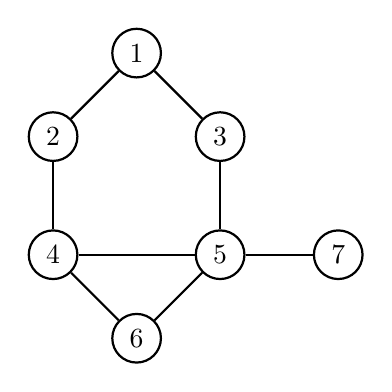
\begin{tikzpicture}[node distance={15mm}, thick, main/.style = {draw, circle}] 
            \node[main] (1) {$1$}; 
            \node[main] (2) [below left of=1] {$2$}; 
            \node[main] (3) [below right of=1] {$3$}; 
            \node[main] (4) [below of=2] {$4$}; 
            \node[main] (5) [below of=3] {$5$};
            \node[main] (6) [below right of=4] {$6$};
            \node[main] (7) [right of=5] {$7$};
            \draw (1) -- (2); 
            \draw (1) -- (3); 
            \draw (2) -- (4);
            \draw (3) -- (5);
            \draw (4) -- (5);
            \draw (4) -- (6);
            \draw (5) -- (6);
            \draw (5) -- (7);
\end{tikzpicture}\newline\newline
\textbf{DFS:} $1 \rightarrow 2 \rightarrow 3 \rightarrow 4 \rightarrow 5 \rightarrow 6 \rightarrow 7$
\begin{itemize}
    \item $L_{0} = \{1\}$
    \item $L_{1} = \{2, 3\}$
    \item $L_{2} = \{4, 5\}$
    \item $L_{3} = \{6, 7\}$
\end{itemize}

\subsection{Correctness}
At the end of BFS($G, s$) we have:
\begin{enumerate}
    \item All the vertices in $C_{s}$ are visited and all the edges are labelled \textit{Discovery Edges} or \textit{Cross Edges}

    \item The set of \textit{Discovery Edges} are a spanning tree $T$ of $C_{s}$ which is called BFS Tree.

    \item $\forall v \in L_{i}$ the path in $T$ from $s$ to $v$ has $i$ edges and every other path from $s$ to $v$ has at least $i$ edges (i.e. $\geq i$ edges)
\end{enumerate}
The proof of the first two properties is the same as for the DFS.\newline\newline
\textbf{Proof of 3:}\newline
Let $P: s = u_{0} \rightarrow u_{1} \rightarrow ... \rightarrow u_{i} = v$ a path from $s$ to $v$, where $u_{j} \in L_{j}$ is \textit{discovered} from the vertex $u_{j - 1} \forall j$. Then, the edge $(u_{j - 1}, u_{j})$ is a \textit{Discovery Edge}. By contradiction, assume assume $\exists$ a path $P': s = z_{0} \rightarrow z_{1} \rightarrow ... \rightarrow z_{t} = v$ with $t < i$. This implies that $ s = z_{0} \in L_{0}$, $z_{1} \in L_{1}$, $z_{2} \in L_{1} \,\, or \,\, L_{2}$, ..., $z_{t} \in L_{1} \,\, or \,\, L_{2} \,\, or \,\,...\,\,L_{t}$. This means that, since $z_{t} = v$, $v \notin L_{i}$, but this is a contradiction.

\subsection{Complexity}
$\forall v \in C_{s}$ there is one iteration of the first \textbf{for} loop and $d(v)$ iterations of the second \textbf{for} loop. Then, the complexity of BFS is:
\[\Theta\left( \sum_{v \in C_{s}} d(v)\right) = \Theta(m_{s})\]

\subsection{Applications}
\begin{itemize}
    \item Same as for DFS in $\Theta(n + m)$ time
    \item Given a graph $G = (V, E)$ and $s,t \in V$ return the \textbf{shortest} path from $s$ to $v$ (if any) \footnote{Shortest path in terms of number of edges between the two nodes}. In order to solve this problem, we can build the path following the same approach as for DFS.
\end{itemize}


\chapter{Lec 04 - Minimum Spanning Tree}

\section{Minimum Spanning Tree (MST)}
\textbf{Definition:}\newline
\begin{itemize}
    \item \textbf{Input:} A graph $G = (V, E)$ undirected, connected, weighted. A weight $w(u, v)$ defines the cost of an edge ($w: E \rightarrow \mathbb{R}$)

    \item \textbf{Output:} A spanning tree $T \subseteq E$ such that $W(T) = \sum_{(u,v) \in T}w(u, v)$ is minimized.
\end{itemize}

Applications of MST are:
\begin{itemize}
    \item Networks (computers, sensors, electrical)
    \item Machine Learning (clustering algorithms)
    \item Computer vision (object detection)
    \item Data mining
    \item Subroutine in other algorithms (approximation algorithms)
\end{itemize}
The simplest MST algorithm is to compute all the spanning trees and select the one with minimum weight. This solution is not possible because the so called \textbf{complete graph}, which is a graph that contains all the $\binom{n}{2}$ possible edges, has $n^{n-2}$ different spanning trees. Then, the algorithm would be exponential in the worst case. \newline\newline
However, MST can be solved in near-linear time using \textbf{greedy algorithms}. We'll see two algorithms that deal with this problem:
\begin{itemize}
    \item Prim's algorithm
    \item Kruskal algorithm
\end{itemize}
They both apply, in different ways, a \textbf{generic greedy algorithm}.

\section{Generic greedy algorithm}
The idea of a generic-MST algorithm is to maintain the following invariant: At each iteration, $A$ is always a subset of edges of some MST. Basically, at each iteration, the algorithm adds an edge that does not violate the invariant (i.e. \textit{safe edge} for $A$).\newline\newline

\textbf{Terminology:}
\begin{itemize}
    \item A \textbf{cut} of a graph $G = (V, E)$ is a partition of the set of vertices. It is usually denoted as $(S, V \setminus S)$.

    \item An edge $(u, v) \in E$ \textbf{crosses} a cut $(S, V \setminus S)$ if $u \in S$ and $v \in V \setminus S$.

    \item A cut \textbf{respects} a set of edges $A$ if no edge of $A$ crosses the cut.

    \item Given a cut, an edge that crosses the cut and is of minimum weight is called \textbf{light-edge}.
    
\end{itemize}

\begin{algorithm}
\caption{Generic MST}\label{Gen.MST}
    \begin{algorithmic}[1]
    \Procedure{Generic-MST ($G$)}{}
        \State $A = \emptyset$
        \While{$A$ does not form a spanning tree}
            \State find an edge $(u, v)$ that is safe for $A$
        \EndWhile
        \Return $A$
    \EndProcedure
    \end{algorithmic}
\end{algorithm}
How can we find a \textit{safe edge} ? Luckily, MSTs enjoy the following structural property:\newline\newline
\textbf{Theorem:} Let $G=(V, E)$ be an undirected, connected and weighted graph. Let $A$ be a subset of $E$ included in some MST of $G$. Let $(S, V \setminus S)$ a cut that respects $A$. Let $(u, v)$ be a light-edge for $(S, V \setminus S)$. Then, $u, v$ is safe for $A$.\newline\newline
\textbf{Termination}: All edges added to $A$ are in a minimum spanning tree, and so the set $A$ must be a minimum spanning tree.\newline\newline
Basically we can iteratively select a cut that respects $A$ and add to $A$ a light-edge according to the cut. Prim and Kruskal algorithms define how to choose a cut.\newline\newline
\textbf{Proof of the theorem:}\newline
Let $T$ be an MST that includes $A$. Assume that $(u, v) \notin T$. We'll build a new MST $T'$ that includes $A \cup \{(u, v)\}$. This would imply that the edge $(u, v)$ is safe for $A$, and the theorem would be demonstrated. By hypothesis, $(u, v)$ crosses the cut $(S, V \setminus S)$. This implies that there exists another edge that crosses $(S, V \setminus S)$. This is because $(u, v) \notin T$, so if no other edge crosses the cut it would mean that $G$ is not connected, which is false by hypothesis. Let $(x, y)$ be such edge. By hypothesis $(S, V \setminus S)$ respects $A$, therefore $(x, y) \notin A$. This implies that by removing $(x,y)$ from $T$ and adding $(u, v)$ we obtain a new spanning tree $T' = T \setminus \{(x, y)\} \cup \{(u, v)\}$ that includes $A \cup \{(u, v)\}$.

Now we need to show that $T'$ not only is a spanning tree, but also a MST. Both $(x, y)$ and $(u, v)$ cross $(S, V \setminus S)$, but by hypothesis $(u, v)$ is a light-edge. This implies that $w(u, v) \leq w(x, y) \rightarrow w(T') = w(T) - w(x, y) + w(u, v) \leq w(T)$. Since $T$ is a MST by hypothesis, it follows that $w(T') = w(T)$.

\section{Prim's alorithm}
Prim's algorithm applies the Generic-MST in the following way:\newpage
\begin{algorithm}
\caption{Prim}\label{Prim}
    \begin{algorithmic}[1]
    \Procedure{Prim ($G, s$)}{}
        \State $X = \{s\}$
        \State $A = \emptyset$
        \While{There is an edge $(u, v)$ with $u \in X$ and $v \notin X$}
            \State $(u^{*}, v^{*})=$ a minimum weight such edge
            \State add $v^{*}$ to $X$
            \State add $(u^{*}, v^{*})$ to $A$
        \EndWhile
        \Return $A$
    \EndProcedure
    \end{algorithmic}
\end{algorithm}
This algorithm \textit{grows} a spanning tree from a source vertex $s$ by adding an edge at a time.
\begin{itemize}
    \item \textbf{Correctness:} it follows from the theorem
    \item \textbf{Complexity:} assume the $G$ is represented with an adjacency list, the complexity is $O(m \cdot n)$, which is polynomial time. Therefore, Prim's algorithm is an efficient algorithm.
\end{itemize}

\chapter{Lec 05 - Informed Search III}
\section{ Simulated annealing}
A hill-climbing algorithm that never makes “downhill” moves toward states with lower value (or higher cost) is guaranteed to be incomplete, because it can get stuck on a local maximum. In contrast, a purely random walk—that is, moving to a successor chosen uniformly at random from the set of successors—is complete but extremely inefficient. Therefore, it seems reasonable to try to combine hill climbing with a random walk in some way that yields both efficiency and completeness. \textbf{Simulated annealing} is such an algorithm. In metallurgy, \textbf{annealing} is the process used to temper or harden metals and glass by heating them to a high temperature and then gradually cooling them, thus allowing the material to reach a low-energy crystalline state.
\begin{center}
    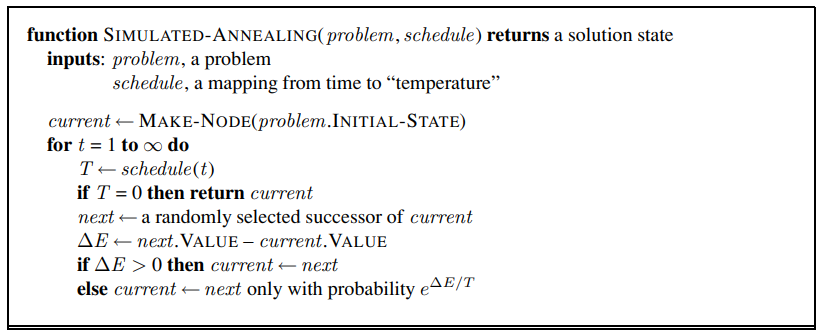
\includegraphics[]{images/annealing.png}
\end{center}
The simulated annealing algorithm is a version of stochastic hill climbing where some downhill moves are allowed. Downhill moves are accepted readily early in the annealing schedule and then less often as time goes on. The schedule input determines the value of the temperature $T$ as a function of time.\newline\newline
The innermost loop of the simulated-annealing algorithm picks a random move. If the move improves the situation, it is always accepted. Otherwise, the algorithm accepts the move with some probability less than 1. The probability decreases exponentially with the “badness” of the move, that is, the amount $\Delta E$ by which the evaluation is worsened. The probability also decreases as the “temperature” $T$ goes down: “bad” moves are more likely to be allowed at the start when $T$ is high, and they become more unlikely as $T$ decreases. If the schedule lowers $T$ slowly enough, the algorithm will find a global optimum with probability approaching 1.

\section{ Local beam search}
The local beam search algorithm keeps track of $k$ states rather than just one. It begins with $k$ randomly generated states. At each step, all the successors of all $k$ states are generated. If any one is a goal, the algorithm halts. Otherwise, it selects the $k$ best successors from the \textbf{complete} list and repeats.\newline\newline
At first sight, a local beam search with $k$ states might seem to be nothing more than running $k$ random restarts in parallel instead of in sequence. However, the two algorithms are quite different. In a random-restart search, each search process runs independently of the others. In a local beam search, useful information is passed among the parallel search threads.\newline\newline
In its simplest form, local beam search can suffer from a lack of diversity among the $k$ states—they can quickly become concentrated in a small region of the state space, making the search little more than an expensive version of hill climbing. A variant called stochastic beam search, analogous to stochastic hill climbing, helps alleviate this problem. Instead of choosing the best $k$ from the the pool of candidate successors, stochastic beam search
chooses $k$ successors at random, with the probability of choosing a given successor being an increasing function of its value.

\section{Genetic algorithms}
A \textbf{genetic algorithm} (or GA) is a variant of stochastic beam search in which successor states are generated by combining two parent states rather than by modifying a single state.\newline\newline
Like beam searches, GAs begin with a set of $k$ randomly generated states, called the \textbf{population}. Each state, or \textbf{individual}, is represented as a string over a finite alphabet, most commonly, a string of 0s and 1s. The production of the next generation of states works as follows:
\begin{enumerate}
    \item Each state is rated by the objective function, or (in GA terminology) the \textbf{fitness function}. A fitness function should return higher values for better states.

    \item for $i=1$ to $size(population)$:

    \begin{enumerate}
        \item A pair is selected at random for reproduction (the probability of being chosen for reproducing is directly proportional to the fitness score). A \textbf{crossover} point is chosen randomly from the positions in the string.

        \item A new child is generated starting from the parents according to the crossover point $c$. Basically, given $n$ the length of the representation string, the child is generated concatenating the substring of the first parent from 1 to $c$ and the substring of the second parent from $c + 1$ to $n$.

        \item Finally, the child is subject to random mutation with a small independent probability and is then added to the new population. 
    \end{enumerate}
     \item Then, the old population is updated to the new population.
    
    
\end{enumerate}


\begin{center}
    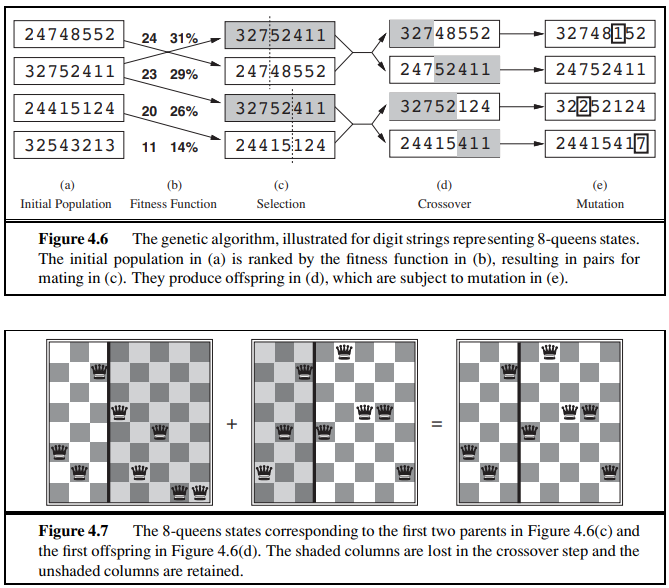
\includegraphics[]{images/GA.png}
\end{center}


\section{Continuous Spaces: Gradient Descent}
Yet none of the algorithms we have described (except for first-choice hill climbing and simulated annealing) can handle continuous state and action spaces, because they have infinite branching factors.\newline\newline
The idea is to minimize/maximize an objective function exploiting its gradient with respect to a set of parameters. The gradient vector can be interpreted as the direction and rate of fastest increase of the function. The gradient is the zero vector at a point if and only if the point is a stationary point.\\\\
This minimization problem can be solved using gradient descent. Starting from a random configuration of $\theta$, each parameter is updated in the following way:
\[\theta_{k+1} = \theta_{k} - \eta \nabla f(\theta_{k})\]
where:
\begin{itemize}
    \item $\nabla f(\theta_{k})$ is the partial derivative of the function in $\theta_{k}$.
    \item The parameter $\eta > 0$ is known as the \textit{learning rate}. 
\end{itemize}
The derivative term $\frac{\partial}{\partial \theta_{k}}f(\theta_{k})$ can be:
\begin{itemize}
    \item $\geq 0$ it means that the function is increasing, so we are decreasing $\theta_{k}$ in the \textit{right direction}.
    \item $\leq 0$ it means that the function is decreasing, so we are increasing $\theta_{k}$ in the \textit{right direction}
\end{itemize}
If $\eta$ is too small, gradient descent can be slow. Anyway, if it is too large, it can overshoot the minimum (fail to converge). 

\section{Online Search}
So far we have concentrated on agents that use \textbf{offline search} algorithms. They compute a complete solution before setting foot in the real world and then execute the solution. In contrast, when the environment is not completely observable, or it is dynamic/semidynamic, the agent needs to interact with the environment to extract information. An \textbf{online search} agent interleaves computation and action: first it takes an action, then it observes the environment and computes the next action. Online search is a necessary idea for unknown environments, where the agent does not know what states exist or what its actions do. In this state of ignorance, the agent faces an \textbf{exploration problem}.\newline\newline

\subsection{Online Search Problems}
We assume a deterministic and fully observable environment, however the agent knows only the following:
\begin{itemize}
    \item ACTIONS($s$), which returns a list of actions allowed in state $s$;

    \item The step-cost function $c(s, a, s')$, note that this cannot be used until the agent knows that $s'$ is the outcome;

    \item GOAL-TEST($s$).
\end{itemize}
If some actions are irreversible the online search might accidentally reach a \textbf{dead-end state}. In general, this is not avoidable (not even for safely explorable state spaces).
\begin{center}
    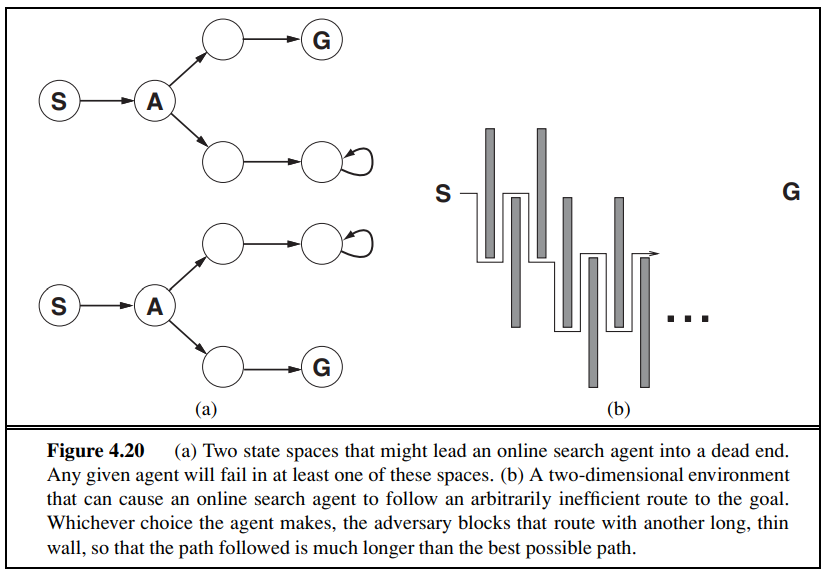
\includegraphics[scale=0.8]{images/dead-end.png}
\end{center}
Typically, the agent’s objective is to reach a goal state while minimizing cost. (Another possible objective is simply to explore the entire environment). The cost is the total path cost of the path that the agent actually travels. It is common to compare this cost with the path cost of the path the agent would follow \textit{if it knew the search space in advance}, that is, the actual shortest path (or shortest complete exploration).  In the language of online algorithms, this is called the \textbf{competitive ratio}; we would like it to be as small as possible.

\subsection{Depth-first Online Search}
After each action, an online agent receives a percept telling it what state it has reached; from this information, it can augment its map of the environment. The current map is used to decide where to go next. Offline algorithms such as A* can expand a node in one part of the space and then immediately expand a node in another part of the space, because node expansion involves simulated rather than real actions. An online algorithm, on the other hand, can discover successors only for a node that it physically occupies. To avoid traveling all the way across the tree to expand the next node, it seems better to expand nodes in a \textbf{local} order.
\newline\newline
Depth-first search has exactly this property because (except when backtracking) the next node expanded is a child of the previous node expanded.
\begin{center}
    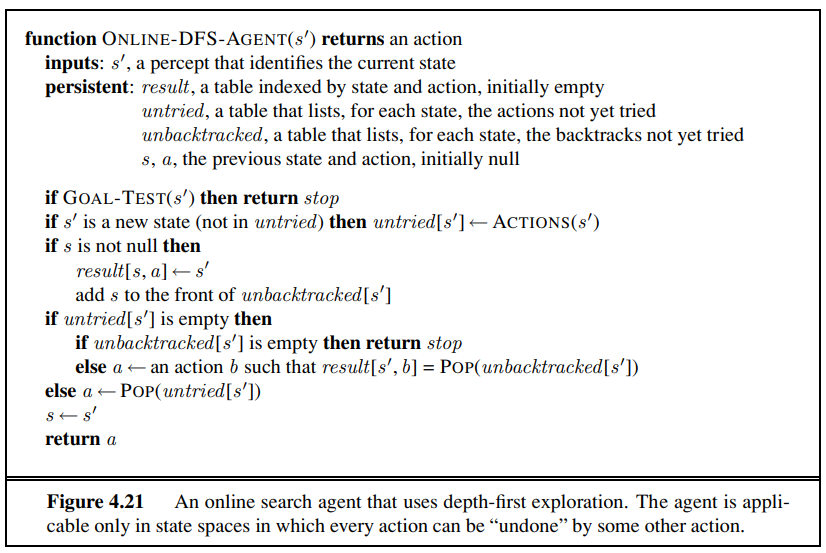
\includegraphics[]{images/online-dfs.png}
\end{center}
This agent stores its map in a table, RESULT[$s, a$], that records the state resulting from executing action $a$ in state $s$. Whenever an action from the current state has not been explored, the agent tries that action. The difficulty comes when the agent has tried all the actions in a state. In offline depth-first search, the state is simply dropped from the queue; in an online search, the agent has to backtrack physically. To achieve that, the algorithm keeps a table that lists, for each state, the predecessor states to which the agent has not yet backtracked. If the agent has run out of states to which it can backtrack, then its search is complete.

\section{Random Search}
Like depth-first search, hill-climbing search has the property of locality in its node expansions. However, random restarts cannot be used, because the agent cannot transport itself to a new state. Instead of random restarts, one might consider using a \textbf{random walk} to explore the environment. A random walk simply selects at random one of the available actions from the current state; preference can be given to actions that have not yet been tried. It is easy to prove that a random walk will eventually find a goal or complete its exploration, provided that the space is finite. On the other hand, the process can be very slow. Augmenting hill climbing with memory rather than randomness turns out to be a more effective approach.

\subsection{LRTA* Search}
The basic idea is to store a “current best estimate” $H(s)$ of the cost to reach the goal from each state that has been visited. $H(s)$ starts out being just the heuristic estimate $h(s)$ and is updated as the agent gains experience in the state space.
\begin{center}
    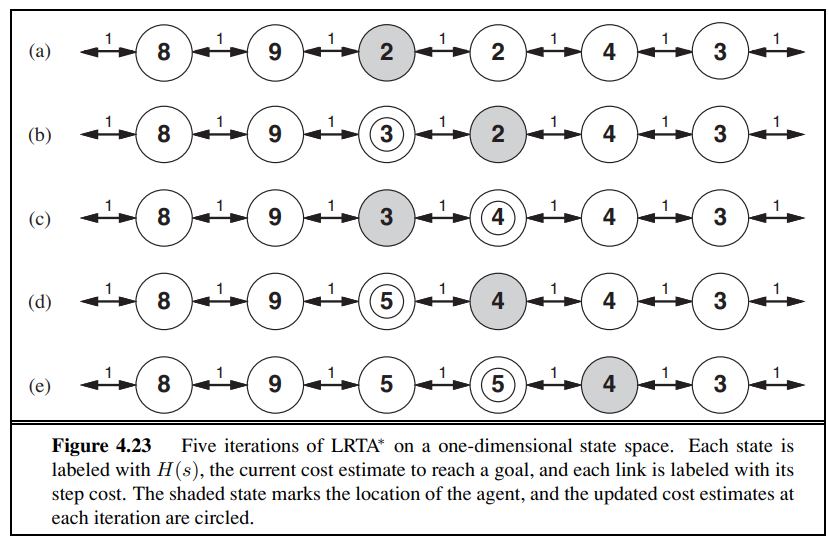
\includegraphics[scale=0.8]{images/LRTA.png}
\end{center}
The agent should follow what seems to be the best path to the goal given the current cost estimates for its neighbors.  The estimated cost to reach the goal through a neighbor $s'$ is the cost to get to $s'$ plus the estimated cost to get to a goal from there, that is, $c(s, a, s') + H(s')$. In the
example, there are two actions, with estimated costs 1+9 and 1+2, so it seems best to move right.\newline\newline
An agent implementing this scheme, which is called learning real-time A* (\textbf{LRTA*}). It builds a map of the environment in the result table. It updates the cost estimate for the state it has just left and then chooses the “apparently best” move according to its current cost estimates. One important detail is that actions that have not yet been tried in a state $s$ are always assumed to lead immediately to the goal with the least possible cost, namely $h(s)$.
\begin{center}
    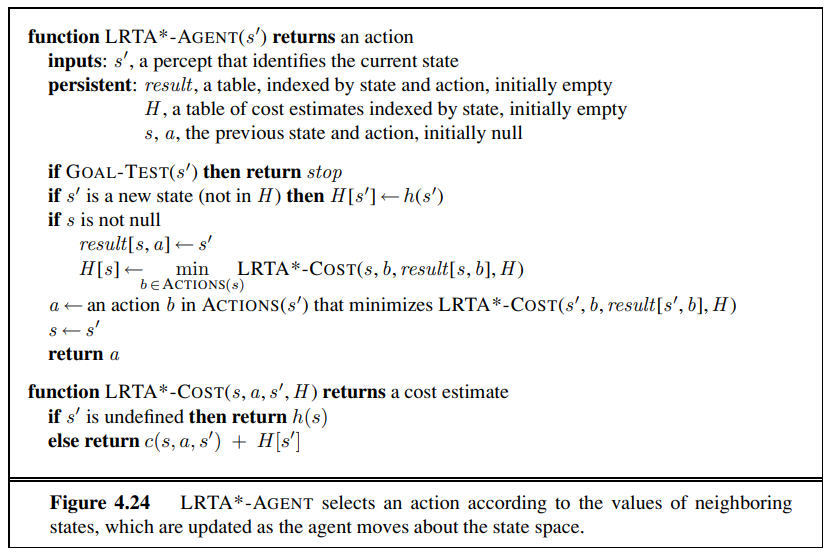
\includegraphics[scale=0.8]{images/LRTA-2.png}
\end{center}

\chapter{Lec 06 - Probability}

\section{Probability - terminology}
\begin{itemize}
    \item \textbf{Random variable:} a variable that can take different values randomly

    \item \textbf{Probability distribution:} a description of how likely a random variable x (or a set of random variables) is to take each of its possible states.\newline\newline
    \textbf{Discrete variables:} Probability distribution is described by a \textbf{Probability mass function}
    \begin{itemize}
        \item The domain of $P$ is the set of all possible states of x ($k$ different values).
        
        \item $\forall \, x \in \text{x} \, 0 \leq P(\text{x} = x) \leq 1$
        
        \item $\sum_{x \in \text{x}}P(x) = 1$
    \end{itemize}
    E.g. Uniform distribution $\forall \, x \in \text{x} \, P(\text{x} = x) = \frac{1}{k}$\newline\newline
    \textbf{Continuous variables:} Probability distribution is described by a \textbf{Probability Density Function} (PDF) 
    \begin{itemize}
        \item The domain of $p$ is the set of all possible states of x

        \item $\forall \, x \in \text{x}\, p(x) \geq 0$

        \item $\int p(x) dx = 1$
    \end{itemize}
    E.g. Gaussian distribution

    \item \textbf{Joint probability distribution:} Probability distribution over 2 or more variables $P(\text{x} = x, \text{y} = y)$

    \item \textbf{Gaussian distribution}: The one-dimensional Gaussian with mean $\mu$ and standard deviation $\sigma$ has the following shape:
    \[G(x) = \frac{1}{\sigma \sqrt{2\pi}}e^{-\frac{(x-\mu)^{2}}{2\sigma^{2}}}\]
    \begin{center}
        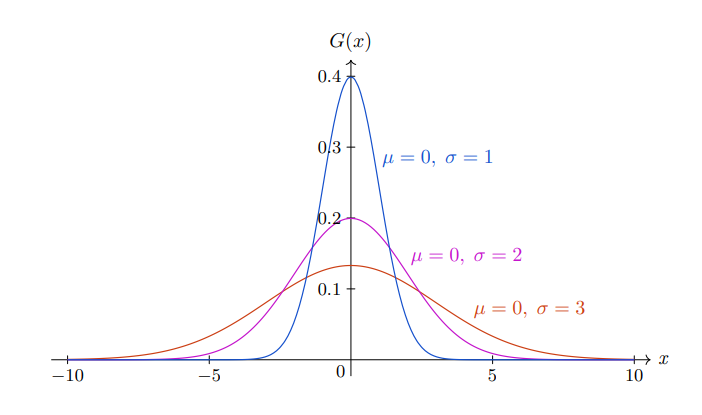
\includegraphics[]{images/Gaussian.png}
    \end{center}

    \item \textbf{Shannon Entropy (discrete variable):} 
    We can apply information theory to calculate the amount of information there is in an event. This is called \textit{self-information} and can be calculated for a \textbf{discrete} event $x$ as follows:
    \[I(x) = -log\,(P(x))\]
    where $log()$ is the base-2 logarithm and $P(x)$ is the probability of the event $x$ \footnote{other bases can be used, $e$ for example}.
    \newline\newline
    The choice of the base-2 logarithm means that the units of the information measure is in bits (binary digits). This can be directly interpreted as the number of bits required to represent an event. If the probability that an event occurs is $0.5$, we need 2 bits two represent it ($0$ fail, $1$ success); if the event occurs with probability $0.125$, we need $3$ bits to represent it (remember $y = log_a\,(x) \iff x = a^y$).
    \newline\newline
    The Shannon entropy of a \textbf{distribution} is the \textbf{expected} amount of information in an event drawn from that distribution:
    \[H(\text{x}) = - E_{x \sim P(\text{x})}[log(P(x))] = -\sum_i P(x_i) log\,P(x_i)\]
    It provides a lower bound on the number of bits needed \textbf{on average} to encode a symbol drawn from the distribution.\newline\newline
    Distributions that are nearly deterministic (where the outcome is nearly certain) have low entropy; distributions that are closer to uniform have high entropy.
    

    \item \textbf{Kullback-Leibler divergence and Cross Entropy:} Let's consider two probability distributions $P(x)$ and $Q(x)$. How can we measure how different they are?
    \begin{itemize}
        \item Kullback-Leiber divergence:
        \[D_{KL}(P \,||\, Q) = E_{x \sim P}\left[ log\frac{P(x)}{Q(x)} \right] = E_{x \sim P}[ log\, P(x) - log\, Q(x)] = \sum_i P(x_i) log\, \left(\frac{P(x_i)}{Q(x_i)}\right)\]
        It is not a true distance because it is not symmetric:
        \[D_{KL}(P \, ||\, Q) \neq D_{KL}(Q \, ||\, P)\]
        It is the measure of information lost when $Q$ is used to approximate $P$.


        \item Cross Entropy:
        \[H(P, Q) = H(P) + D_{KL}(P\, ||\, Q) = -E_{x \sim P}[log\, Q(x)]\]
        where $H(P)$ is the entropy of $P$. Note that minimizing the Cross Entropy of $P$ with respect to $Q$ is equivalent to minimize KL divergence between $P$ and $Q$. (if $P$ is given, $H(P)$ and $E_{x \sim P}[log\, P(x)]$ are constants). If $P$ is a fixed distribution minimize KL divergence or minimize CE is the same, but CE is easier to compute.
    \end{itemize}

    \item \textbf{Maximum likelihood estimation:} Is a principled way to derive estimators (models). Consider $n$ examples $Tr = \{\textbf{x}^{1}, ..., \textbf{x}^{n}\}$ drawn i.i.d. from $p_{data}$ (which is not known in advance). With machine learning we want to estimate this probability $p_{data}$ with some models that depend on a set of parameters $\theta$.\newline\newline
    Let's consider a family of parametric probability distributions (models) $p_{model}(\textbf{x}; \theta)$. It maps a point $\textbf{x}$ to a real number, estimating $p_{data} (\textbf{x})$. How can we find $\theta$ in such a way that $p_{model}$ and $p_{data}$ are as close as possible ? A possible formalization of this problem is given by the Maximum Likelihood estimation for $\theta$:
    \[\theta_{ML} = argmax_{\theta}\, p_{model}(Tr; \theta) = argmax_{\theta}\prod_{i = 1}^{n}p_{model}(\textbf{x}^{i}; \theta)\]
    Basically, we choose the probability distribution which is most likely to have produced our data. Note that we are assuming that all the examples are \textbf{independent} each other ($P(x, y) = P(x)P(y)$).
\end{itemize}

\section{Maximum likelihood}
Maximum likelihood (ML) is a special case of \textbf{maximum a posteriori estimation (MAP)}.
\[h_{MAP} = argmax_{h \in H}P(h|D)\]
\[= argmax_{h \in H}\frac{P(D|h)P(h)}{P(D)}\]
where:
\begin{itemize}
    \item $P(h):$ a priori probability of the hypothesis $h$
    \item $P(D):$ a priori probability of training data. It is the probability to observe exactly this training set when we don't know anything about the hypothesis.
    \item $P(h|D):$ probability of $h$ given $D$. It is the probability that $h$ is the hypothesis that generates data $D$.
    \item $P(D|h):$ probability if $D$ given $h$. Given a hypothesis $h$, it is the probability of data $D$ to be generated by $h$.
\end{itemize}
Since $P(D)$ does not depend on $h$, we can consider it as a constant and remove it from the equation.
\[= argmax_{h \in H}P(D|h)P(h)\]
If we assume uniform probabilities on the hypotheses, that is $P(h_{i}) = P(h_{j})$, we can choose the so called \textbf{maximum likelihood hypothesis} $h_{ML}:$
\[h_{ML} = argmax_{h \in H}P(D|h)\]
MAP and maximum likelihood approach make predictions using a single point estimate of $\theta$. The Bayesian approach is to make predictions using a full probability distribution over $\theta$. For example, given a new instance $\textbf{x}$, which is the most likely \textbf{classification}? The classification given by the most likely hypothesis $h_{MAP}$ is not necessarily the most likely classification. For example, given the following three possible hypothesis:
 \[P(h_{1} | D) = 0.4 \quad P(h_{2} | D) = 0.3 \quad P(h_{3} | D) = 0.3\]
 We want to classify a new instance $\textbf{x}$:
 \[h_{1}(\textbf{x}) = + \quad h_{2}(\textbf{x}) = - \quad h_{1}(\textbf{x}) = -\]
 The most likely hypothesis $h_{1}$ classifies $\textbf{x}$ with the label (+), but the most likely classification is (-). This is because the optimal (Bayes) classification of a certain instance is the class $v_{j} \in V$ which maximizes the following probability:
 \[argmax_{v_{j} \in V} = \sum_{h_{i} \in H}P(v_{j} | h_{i})P(h_{i} | D)\]
 where $V$ is the set of possible labels.\newline\newline
 However, in real-world problems having the probabilities $P(h_{i} | D)$ is almost impossible. Therefore, we usually make the assumption of considering the classification made by $h_{map}$ as most probable.

 \subsection{Maximum likelihood estimation}
 As we said before, the maximum likelihood estimation is defined as follows:
 \[\theta_{ML} = argmax_{\theta}\, p_{model}(Tr; \theta) = argmax_{\theta}\prod_{i = 1}^{n}p_{model}(\textbf{x}^{i}; \theta)\]
 However, computing the product of many probability is unstable. Therefore, we can apply the $log$ and the $argmax$ does not change (log-likelihood).
 \[\theta_{ML} = log(argmax_{\theta}\prod_{i=1}^{n}p_{model}(\textbf{x}^{(i)}; \theta))\]
 \[= argmax_{\theta}\sum_{i = 1}^{n}log\, p_{model}(\textbf{x}^{(i)}, \theta)\]
 We can equivalently divide by $n$ to express maximum likelihood as an expectation over training data:
 \[\theta_{ML} = argmax_{\theta}E_{x \sim \hat{p}_{data}}[log \, p_{model}(x; \theta)]\]
where $\hat{p}_{data}$ is an empirical discrete distribution that we get over the examples in the training set. This implies that maximum likelihood minimizes the dissimilarity between $\hat{p}_{data}$ and $p_{model}$, measured by the KL divergence. It also corresponds to minimize the \textbf{cross-entropy} between the two distributions.

\subsection{Conditional log likelihood}
We can use maximum likelihood to estimate a \textbf{conditional} probability $P(\textbf{y} | \textbf{x}; \theta)$ to predict $\textbf{y}$ given $\textbf{x}$ (supervised learning).
\[\theta_{ML} = argmax_{\theta} P(\textbf{Y} | \textbf{X}; \theta)\]
If input examples are i.i.d.
\[\theta_{ML} = argmax_{\theta}\sum_{i=1}^{n}log\, P(\textbf{y}^{(i)} | \textbf{x}^{(i)}; \theta)\]
Consider any real-valued target function $f$ and learning examples $\langle 
 \textbf{x}_{i}, d_{i}\rangle$ where $d_{i}$ has some noise:
 \begin{itemize}
     \item $d_{i} = f(\textbf{x}_{i}) + e_{i}$
     \item $e_{i}$ is a random variable (noise) extracted independently, for each $\textbf{x}_{i}$, according to a Gaussian distribution with mean 0.
 \end{itemize}
 It can be shown that the maximum likelihood hypothesis is the one that minimizes the mean squared error:
 \[\theta_{ML} = argmin_{\theta} \sum_{i=0}^{m}(d_{i} - \hat{y}_{i})^{2}\]
maximizing the log-likelihood with respect to $\theta$ yields the same estimate of the parameters $\theta$ as does minimizing the mean squared error.

\chapter{Lec 07 - Neural Networks I}

\section{Neural Networks}
An artificial neuron is a unit that computes a non-linear function over the inputs. Its output depends on the input and on the set of \textbf{weights}. These weights have to be learned.\newline\newline
An \textbf{Artificial Neural Network} is a system consisting of interconnected units that compute nonlinear (numerical) functions. Adjustable weights are associated with connections among units.\newline\newline
Deep Feed Forward Neural Networks, also called multi-layer perceptrons (MLP), approximate a function $f^{*}$ that maps an input $x$ to a category $y$. The MLP defines a mapping $\hat{y} = f(x;\theta)$ where $\theta$ is the set of parameters. They are typically represented as a composition of many different functions $f(x) = f^{(3)}(f^{(2)}(f^{(1)}(x)))$. The intermediate layers are called \textbf{hidden layers}, while the final layer is called \textbf{output layer}.\newline\newline
Multiple layers of cascaded units makes a Neural Network able to implement complex non linear functions. The non linearity of the model is given by the activation functions. In fact, without them (linear activation) the result of the model, even if it’s very complex, would still be linear.\newline\newline
\textbf{Example:}\newline
Let's try to define a linear model that predicts the XOR function.
\[Tr = \{ ([0,0], 0), ([0, 1], 1), ([1,0],1), ([1,1], 0)\} \quad f(\textbf{x};\textbf{w};b) = \textbf{x}\textbf{w}^{T} + b\]
The XOR function \textbf{cannot} be learned by any linear classifier. In order to solve this problem, we can define a two-layers Neural Network with the addition of the ReLU activation function $ReLU(y) = max(0, y)$. The networks becomes:
\[f(\textbf{x}; \textbf{W}, \textbf{c}, \textbf{w}, b) = \textbf{w}^{T} \, max(0, \textbf{W}\textbf{x}^{T} + \textbf{c}) + b\]
the following parameters values provide a solution to the XOR problem:
\[
    \textbf{W} =
    \begin{bmatrix}
        1 & 1\\
        1 & 1
    \end{bmatrix},
    \,\,
    \textbf{c} = 
    \begin{bmatrix}
        0 \\
        -1
    \end{bmatrix},
    \,\,
    \textbf{w} = 
    \begin{bmatrix}
        1 \\
        -2
    \end{bmatrix},
    \,\,
    b = 0
\]
Note that the first hidden layer has two nodes.\newline\newline
The most common activation functions are the following:
\begin{center}
    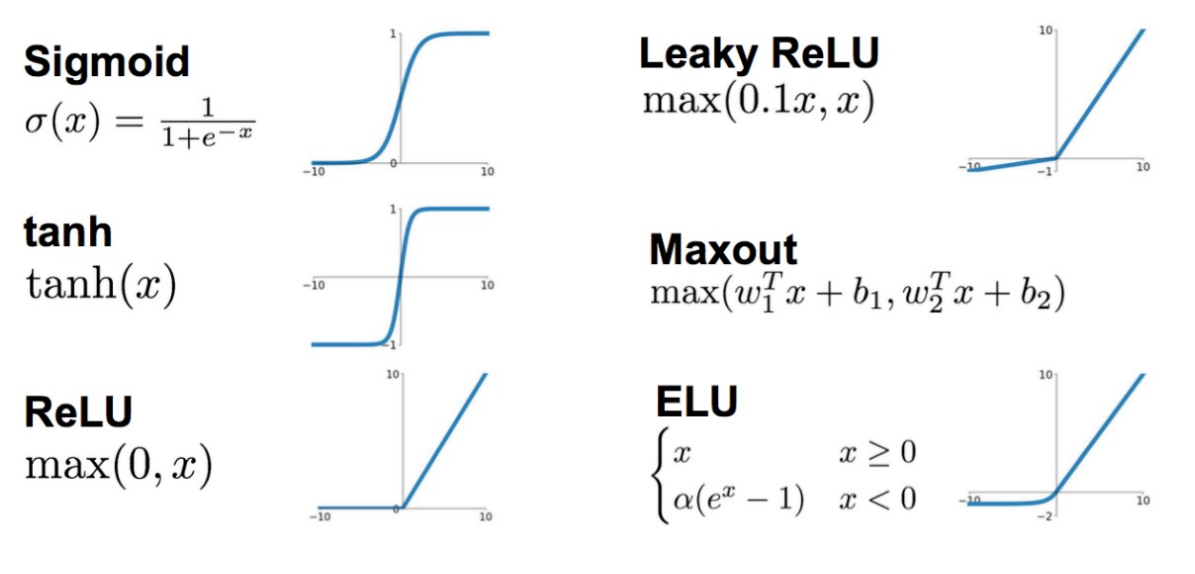
\includegraphics[scale = 0.6]{images/Activation Functions.png}
\end{center}
In general, the goal is to have a more complex decision surface. We can achieve this goal by using non-linear activation functions and stacking several hidden layers. In the XOR example above, the initial points are mapped by the first hidden layer into a new space where they are linearly separable. Thanks to this, the output linear layer is able to classify the points correctly.

\section{Learning in a Neural Network}
In general, the problem of how to update the weights of a model in order to minimize the committed error is called \textbf{credit assignment problem}. A possible solution is to make a single neuron \textbf{derivable} and exploit gradient descent technique to learn the \textit{right} weights. In order to make a neuron derivable, its activation function must be derivable.\newline\newline
Linear models (e.g. SVM) are formulated as \textbf{convex models}. However, the non-linearity in neural networks makes the problem \textbf{non-convex}. It means that there is no guarantee of achieving the global optimum. Furthermore, the way in which the weight of a NN are initialized has a strong impact on the solution that the model will find.

\section{Cost Function}
A important aspect of the design of a deep neural network is the choice of the cost function. In most cases, the model defines a distribution $p(\textbf{y} | \textbf{x}; \theta)$ and the cost function is the cross-entropy between training labels and network predictions (negative log-likelihood):
\[J(\theta) = - E_{(x,y) \sim \hat{p}_{data}}log\, p_{model}(\textbf{y}|\textbf{x})\]
The specific form of the cost function changes from model to model. The output representation $\textbf{h} = f(\textbf{x};\theta)$ determines the form of the cross-entropy function.
\begin{itemize}
    \item \textbf{Linear Regression:} If we assume that the target values are distributed according to a Gaussian distribution $G$, we can think our output layer as to produce the mean of $G$.
    \[\hat{\textbf{y}} = \textbf{W}^{T}\textbf{h} + \textbf{b}\]
    \[G(\textbf{y};\hat{\textbf{y}}; \textbf{I})\]
    As we already seen, in this case maximizing the likelihood corresponds to minimize the mean squared error.
    \[J(\theta) = \frac{1}{2}E_{p \sim \hat{p}_{data}}(y - f(\textbf{x}; \theta))^{2} + constant\]
    Basically, this is a motivation of why the mean squared error cost function is suitable for linear regression.

    \item \textbf{Binary classification:} In this case we assume that our targets are distributed according to a Bernoulli distribution. This distribution depends on a single parameter $\phi \in [0, 1]$:
    \begin{itemize}
        \item $P(\text{x} = 1) = \phi$
        \item $P(\text{x} = 0) = 1 - \phi$
    \end{itemize}
    In general:
    \[P(\text{x} = x) = \phi^{x}(1 - \phi)^{1-x}\]
    The NN just needs to predict $P(\text{y} = 1 | \textbf{x})$. Therefore, we want to force this number to lie in $[0, 1]$. For example, we can use the following function:
    \[P(\text{y} = 1|\textbf{x}) = max(0, min(1, \textbf{w}^{T}\textbf{h} + b))\]
    However, this is not a good choice for gradient descent. In fact, if the output is outside $[0, 1]$ the function is not derivable and the gradient will always be 0. We want to ensure that there is always some gradient when the model is wrong. An alternative way to force the output to lie in $[0, 1]$ is to use an \textbf{output} linear layer with a \textbf{sigmoid activation function}.
    \[\hat{y} = \sigma(\textbf{w}^{T}\textbf{h} + b)\]
    where $\sigma$ is a Sigmoid or Logistic function:
    \[\sigma(x) = \frac{1}{1 + e^{-x}}\]
    \begin{center}
        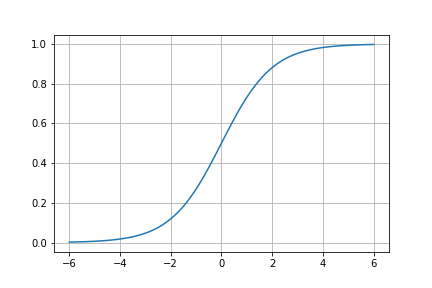
\includegraphics[scale = 0.5]{images/sigmoid.png}
    \end{center}
    An output unit is composed of two components:
    \begin{itemize}
        \item $z = \textbf{w}^{T}\textbf{h} + b$
        \item $\sigma(\cdot)$: the activation function to \textbf{convert $z$ into a probability} (in order to apply maximum likelihood optimization).
    \end{itemize}
    How can we define a probability distribution over $y$ using the value $z$ ? The sigmoid can be motivated by constructing an unnormalized probability distribution $\hat{P}(y)$, which does not sum to 1. We assume that the unnormalized probabilities are linear in $y$ and $z$.
    \[log\, \hat{P}(y) = yz \quad i.e. \,\, log\, \hat{P}(y = 1) = z, \,\, log\, \hat{P}(y = 0) = 0\]
    We can exponentiate to obtain the unnormalized probabilities:
    \[\hat{P}(y) = e^{yz}\]
    Then, we normalize to obtain a proper probablity:
    \[P(y) = \frac{e^{yz}}{\sum_{y'=0}^{1} e^{y'z}} = \sigma((2y - 1)z)\]
    where:
    \begin{itemize}
        \item $P(y = 1) = \frac{1}{1 + e^{-z}}$
        \item $P(y = 0) = \frac{1}{1 + e^{z}}$
    \end{itemize}
    As we already seen, the cost function used with maximum likelihood is the negative-log likelihood. Therefore, the loss function for maximum likelihood learning of a Bernoulli parametrized by a sigmoid is:
    \[J(\theta) = -log\, P(y|\textbf{x}) = -log\,\sigma((2y - 1)z) = \zeta((1 - 2y)z)\]
    where $\zeta(x) = log(1 - exp(x))$ is called \textbf{softplus} function.\newline\newline
    This approach to predicting the probabilities in log-space is natural to use with maximum likelihood learning. The log in the cost function undoes the exp of the sigmoid. Without this effect, the saturation of the sigmoid could prevent gradient- based learning from making good progress.\newline\newline
    The saturation (i.e. when the gradient is very small) occurs when $y = 1$ and $z$ is very positive or $y = 0$ and $z$ is very negative, that is, when the model has the right answer.\newline\newline
    With other cost functions, such as MSE, we'll be able to find a solution but it would \textbf{not} be the maximum-likelihood solution.

    \item \textbf{Multi-class classification:} In this case the output has to be a probability distribution over a discrete variable with $n$ possible values. We have to generate a vector $\hat{\textbf{y}}= [\hat{y}_0, \hat{y}_1, ..., \hat{y}_{n-1}]$ where:
    \begin{itemize}
        \item $\hat{y}_i = P(y = i | \textbf{x})$
        \item $\forall i,\,\, 0 \leq \hat{y}_i \leq 1$
        \item $\sum_i \hat{y}_i = 1$
    \end{itemize}
    We can use the same approach for the Bernoulli distribution generalized to the \textbf{Multinoulli distribution}:
    \[\textbf{z} = \textbf{W}^{T}\textbf{h} + \textbf{b} \quad \text{where}\,\, z_i = log\, \hat{P}(y = i | x)\]
    In order to represent the probability distribution over $n$ different classes, we can use the \textbf{Softmax} function, which is a generalization of sigmoid.
    \[softmax(\textbf{z})_i = \frac{e^{z_i}}{\sum_j^n e^{z_j}}\]
    By applying the log-likelihood, the cost function is:
    \[log\, softmax(\textbf{z})_i = z_i - log \, \sum_j e^{z_j}\]
    $z_i$ pushes the correct labels up and $log \, \sum_j e^{z_j}$ pushes the uncorrect labels down. When we perform the prediction, we'll choose the argmax of $\hat{\textbf{y}}$.
\end{itemize}

\subsection{Output functions in general}
Linear, sigmoid and softmax output units are the most common, but NN can generalize to almost any kind of output layer.\newline\newline
Maximum likelihood provides a guide to design almost any output layer.
\begin{enumerate}
    \item We define a conditional distribution $p(\textbf{y}|\textbf{x}; \theta)$
    \item As cost function, maximum likelihood suggest to use $-log\, p(\textbf{y}|\textbf{x}; \theta)$
\end{enumerate}
We can think of the NN as $f(\textbf{x}; \theta) = \omega$ where $\omega$ are the parameters of a distribution over $\textbf{y}$ and the cost function is $-log\, p(\textbf{y};\omega(\textbf{x}))$

\section{Hidden units}
An hidden unit can be described as accepting an input $x$, computing $z = W^{T}x + b$, and applying an element-wise nonlinear function $g(z)$. The design of hidden units does not have many definitive guiding theoretical principle. What we can do is to evaluate hidden units performance on a validation set. To select the most suitable activation function we can rely on some basic intuitions motivating each type of hidden unit.

\subsection{Hidden units: ReLU}
An hidden unit with ReLU activation function is defined as follows:
\[g(z) = max(0, z) \quad z = f(\textbf{W}^{T}\textbf{x} + \textbf{b})\]
Such hidden units are similar to linear units and therefore easier to optimize. However, ReLU units do not learn via gradient-based methods on examples for which their activation is zero. In order to solve this problem, generalizations of ReLU have been defined (e.g. leakyReLU) $g(z, \alpha)_i = max(0, z_i) + \alpha_i \, min(0, z_i)$.

\subsection{Hidden units: Tanh and sigmoid}
Other common activation functions are Tanh and sigmoid:
\begin{itemize}
    \item Logistic sigmoid: $g(z) = \sigma(z)$
    \item Hyperbolic Tangent: $g(z) = tanh(z) = 2\sigma(2z) - 1$
\end{itemize}
Actually, these two functions are not a very good choice for the hidden layers since they saturate across most of their domain. In particular, they saturate to high value when $z$ is very positive, and to low value when $z$ is very negative. This is good for output units, as we seen before, but not for hidden units, because in hidden layers we just want to keep learning without necessarily having a value between 0 and 1. Tanh typically performs better than the logistic sigmoid.\newline\newline
In general, many differentiable functions are reasonable (e.g. $cos(x)$), but they show no significant advantage over common ones.

\section{Architecture}
The architecture of a NN is its overall structure. Neural networks are generally organised in layers where each layer is a function of the preceding one:
\[\textbf{h}^{(1)} = g^{(1)}(\textbf{W}^{(1)T}\textbf{x} + \textbf{b}^{(1)})\]
\[\textbf{h}^{(i)} = g^{(i)}(\textbf{W}^{(i)T}\textbf{h}^{(i - 1)} + \textbf{b}^{(i)})\]
The main architectural considerations are:
\begin{itemize}
    \item The depth of the network
    \item The width of each layer
\end{itemize}
Deeper networks tend to generalize better, but they are harder to train.\newline\newline
All these hyper-parameters should be validated on a validation set.\newline\newline
\textbf{Universal approximation Theorem}\newline\newline
Given a feed-forward NN with just one hiddel layer, any continuous function $f:\mathbb{R}^{n} \rightarrow \mathbb{R}$ and an arbitrarily small $\epsilon > 0$, then, for a large class of activation functions, there always exists an integer $M$ such that the function $g: \mathbb{R}^{n} \rightarrow \mathbb{R}$ computed by the net using at least $M$ hidden units approximates the function $f$ with tolerance $\epsilon$, that is:
\[max_{x \in \Omega}|f(\textbf{x}) - g(\textbf{x})| < \epsilon\]
Note that the theorem attests the existence of a NN with $M$ hidden units that approximates any continuous function with the desired tolerance, but it says nothing about how $M$ can be computed and how large this network would be. Furthermore, we are not guaranteed that the training algorithm will be able to learn it (the optimization algorithm may not be able to find the value of the parameters that corresponds to the desired function).\newline\newline
Using deeper models can reduce the number of units required to represent the desired function. Furthermore, greater depth does seem to result (empirically) in better generalization for a wide variety of tasks.\newline\newline
Many neural networks architectures have been developed for specific tasks, e.g. Convolutional Neural Networks (CNN) or Recurrent Neural Network (RNN). In general, the layers need to be connected in a chain:
\begin{itemize}
    \item Skip connections: Make it easier for the gradient to flow from output layers to layers nearer the input.

    \item Sparse connections: Each unit in a layer is connected to only a small subset of units in the next layer.
\end{itemize}

\chapter{Lec 08 - Logical Agents}
\section{Logical Agents}
Logical agents simulate the process of \textbf{reasoning} operating on internal \textbf{representations} of knowledge. The problem-solving agents seen so far know things, but only in a very limited,
inflexible sense. The knowledge of what the actions do is hidden inside the domain-specific code of the transition model, which defines the result of a move. We will see that \textbf{logic} provides a possible formalism to support knowledge-based agents.

\section{Knowledge based agents}
The central component of a knowledge-based agent is its \textbf{knowledge base}, or KB. A knowledge base is a set of \textbf{sentences} in a formal language. Each sentence is expressed in a language called a \textbf{knowledge representation language} and represents some assertion about the world.\newline\newline
There must be a way to add new sentences to the knowledge base and a way to query what is known. The standard names for these operations are TELL and ASK, respectively. Both operations may involve inference, that is, deriving new sentences from old.\newline\newline
Agents can be viewed at the \textbf{knowledge level}, that is, what they know, regardless of how implemented, or can be viewed  at the implementation level, data structures in KB and algorithms that manipulate them.
\begin{center}
    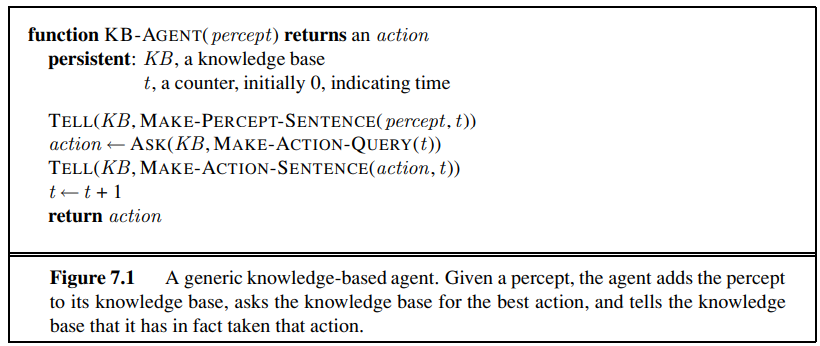
\includegraphics[]{images/KB-agents.png}
\end{center}
The figure above shows the outline of a knowledge-based agent program. Like all our agents, it takes a percept as input and returns an action. The agent maintains a knowledge base, KB, which may initially contain some \textbf{background knowledge}.\newline\newline
Each time the agent program is called, it does three things. First, it TELLs the knowledge base what it perceives. Second, it ASKs the knowledge base what action it should perform. In the process of answering this query, extensive reasoning may be done about the current state of the world, about the outcomes of possible action sequences, and so on.
Third, the agent program TELLs the knowledge base which action was chosen, and the agent executes the action. In order to do so, the agent must be able to:
\begin{itemize}
    \item Represent states, actions, etc.
    \item Incorporate new percepts
    \item Update internal representations of the world
    \item Deduce hidden properties of the world
    \item Deduce appropriate actions
\end{itemize}

\section{The Wumpus world}
In this section we describe an environment in which knowledge-based agents can show their worth. The \textbf{wumpus world} is a cave consisting of rooms connected by passageways. Lurking somewhere in the cave is the terrible wumpus, a beast that eats anyone who enters its room. The wumpus can be shot by an agent, but the agent has only one arrow. Some rooms contain bottomless pits that will trap anyone who wanders into these rooms (except for the wumpus, which is too big to fall in). The only mitigating feature of this bleak environment is the possibility of finding a heap of gold.
\begin{center}
    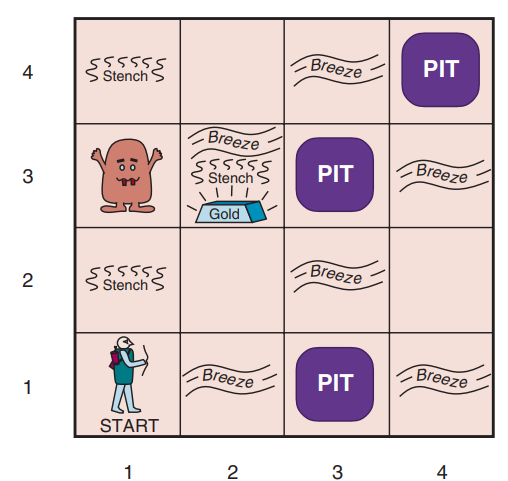
\includegraphics[]{images/wumpus.png}
\end{center}
The precise definition of the task environment is given by the PEAS description:
\begin{itemize}
    \item \textbf{Performance measure}: +1000 for climbing out of the cave with the gold, -1000 for falling into a pit or being eaten by the wumpus, -1 for each action taken and -10 for using up the arrow. The game ends either when the agent dies or when the agent climbs out of the cave.

    \item \textbf{Environment:} A $4 \times 4$ grid of rooms. The agent always starts in the square labeled $[1,1]$, facing to the right. The locations of the gold and the wumpus are chosen randomly, with a uniform distribution, from the squares other than the start square. In addition, each square other than the start can be a pit, with probability 0.2.

    \item \textbf{Actuators:} The agent can move \textit{Forward}, \textit{TurnLeft} by $90^{\circ}$, or \textit{TurnRight} by $90^{\circ}$. The agent dies a miserable death if it enters a square containing a pit or a live wumpus. The action \textit{Grab} can be used to pick up the gold if it is in the same square as the agent. The action \textit{Shoot} can be used to fire an arrow in a straight line in the direction the agent is facing (only one available). Finally, the action \textit{Climb} can be used to climb out of the cave, but only from square $[1,1]$.

    \item \textbf{Sensors:} The agent has five sensors, each of which gives a single bit of information:
    \begin{itemize}
        \item In the square containing the wumpus and in the directly (not diagonally) adjacent squares, the agent will perceive a \textit{Stench}.

        \item In the squares directly adjacent to a pit, the agent will perceive a \textit{Breeze}.

        \item In the square where the gold is, the agent will perceive a \textit{Glitter}.

        \item When an agent walks into a wall, it will perceive a \textit{Bump}.

        \item  When the wumpus is killed, it emits a woeful \textit{Scream} that can be perceived anywhere in the cave.
    \end{itemize}
\end{itemize}
We can characterize the wumpus environment along the various dimensions seen previously. It is discrete, static, and single-agent. It is sequential, because rewards may come only after many actions are taken. It is partially observable, because some aspects of the state are not directly perceivable. For an agent in the environment, the main challenge is its initial ignorance of the configuration of the environment.  Overcoming this ignorance seems to require logical reasoning.\newline\newline
Let us watch a knowledge-based wumpus agent exploring the environment using an informal knowledge representation language consisting of writing
down symbols in a grid:
\begin{center}
    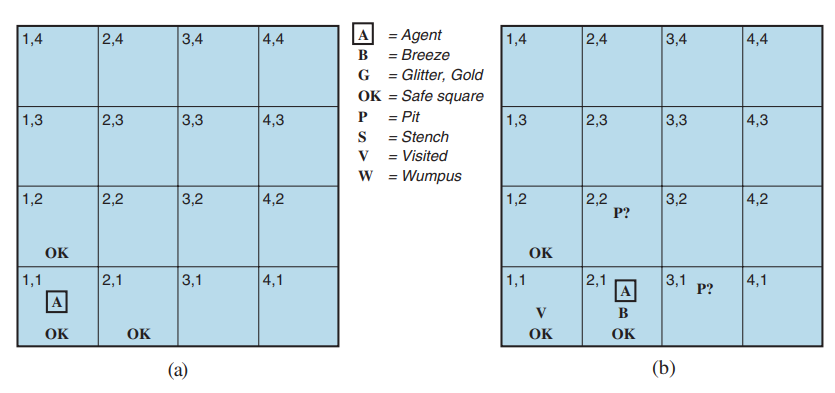
\includegraphics[scale=0.8]{images/wumpus-grid.png}
    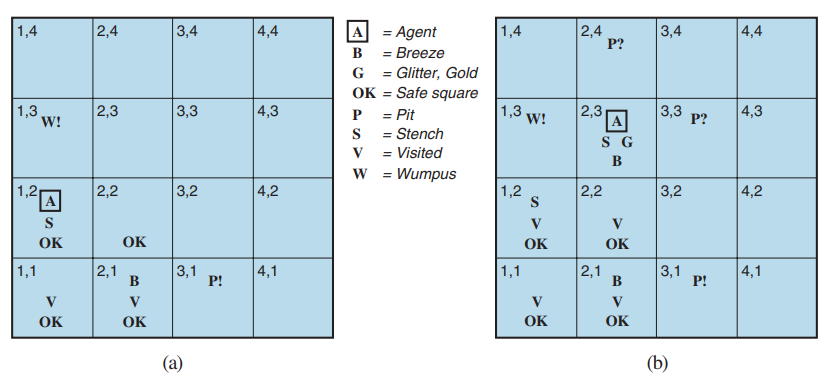
\includegraphics[scale=0.8]{images/wumpus-grid2.png}
\end{center}
Note that in each case for which the agent draws a conclusion from the available information, that conclusion is guaranteed to be correct if the available information is correct. we'll describe how to build logical agents that can represent in a \textbf{formal way} information and draw conclusions.

\section{Propositional Logic}
We now present a simple but powerful logic called \textbf{propositional logic}. The \textbf{syntax} of propositional logic defines the allowable sentences. The \textbf{atomic sentences} consist of a single proposition symbol (P, Q, R, ... but can be whatever). Each such symbol stands for a proposition that can be true or false. There are two proposition symbols with fixed meanings: \textit{True} is the always-true proposition and \textit{False} is the always-false proposition. \textbf{Complex sentences} are constructed from simpler sentences, using parentheses and \textbf{logical connectives}.
\begin{center}
    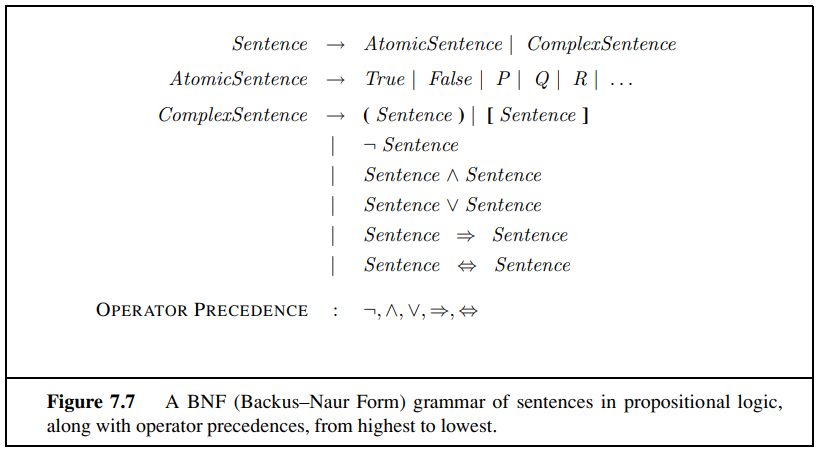
\includegraphics[scale=0.8]{images/BNF.png}
    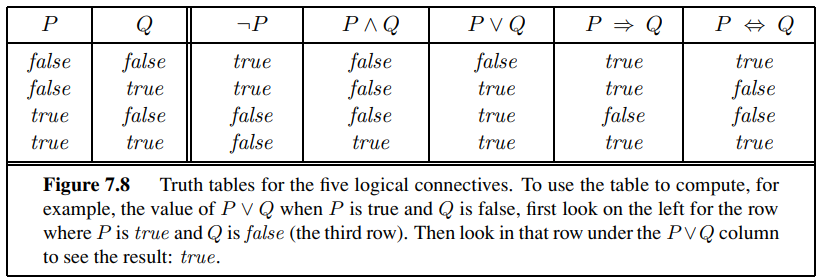
\includegraphics[scale=0.8]{images/truth-table.png}
\end{center}

\section{Models}
As we said previously, the knowledge bases consist of sentences. These sentences are expressed according to the \textbf{syntax} of the representation language, which specifies all the sentences that are well formed. A logic must also define the \textbf{semantics} or meaning of sentences. The semantics defines the truth of each sentence with respect to each possible world.\newline\newline
When we need to be precise, we use the term \textbf{model} in place of “possible world.”  If a sentence $\alpha$ is true in model $m$, we say that $m$ \textbf{satisfies} $\alpha$ or sometimes $m$ \textbf{is a model of} $\alpha$. We use the notation $M(\alpha)$ to mean the set of all models of $\alpha$. Basically, a model assigns truth values to proposition symbols of a sentence.\newline\newline
Now that we have a notion of truth, we are ready to talk about logical reasoning. This involves the relation of logical \textbf{entailment} between sentences, —the idea that a sentence follows logically from another sentence. In mathematical notation, we write:
\[\alpha \vDash \beta\]
to mean that the sentence $\alpha$ entails the sentence $\beta$. The formal definition of entailment is this: $\alpha \vDash \beta$ if and only if, in every model in which $\alpha$ is true, $\beta$ is also true. Using the notation just introduced, we can write
\[\alpha \vDash \beta\,\, \text{if and only if } M(\alpha) \subseteq M(\beta)\]
Note that the direction of the $\subseteq$ means that $\alpha$ is a stronger assertion than $\beta$.\newline\newline
We can apply the same kind of analysis to the wumpus-world reasoning example given previously. The agent has detected nothing in $[1,1]$ and a breeze in $[2,1]$. These percepts, combined with the agent’s knowledge
of the rules of the wumpus world, constitute the KB. The agent is interested (among other things) in whether the adjacent squares $[1,2]$, $[2,2]$, and $[3,1]$ contain pits. Each of the three squares might or might not contain a pit, so (for the purposes of this example) there are $2^3 = 8$ possible models.
\begin{center}
    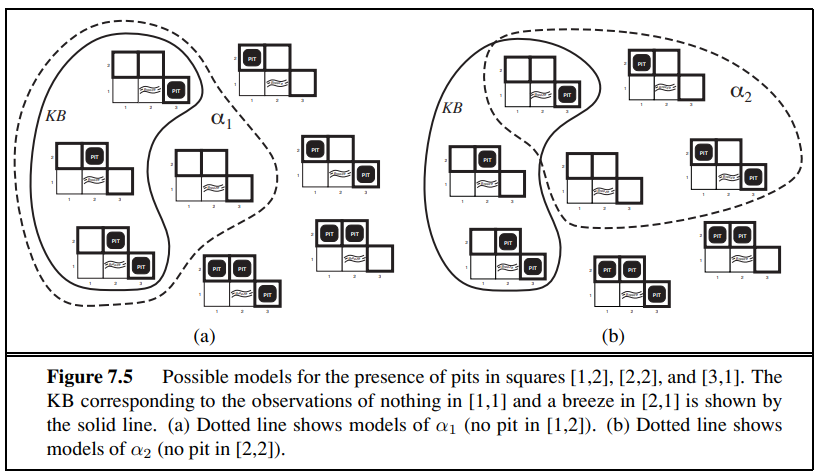
\includegraphics[scale=0.8]{images/kb-wumpus.png}
\end{center}
The KB can be thought of as a set of sentences or as a single sentence that asserts all the individual sentences. The KB is false in models that contradict what the agent knows; for example, the KB is false in any model in which $[1,2]$ contains a pit, because there is no breeze in $[1,1]$. There are in fact just three models in which the KB is true, and these are shown surrounded by a solid line in the figure above.\newline\newline
Now let us consider two possible conclusions:
\begin{itemize}
    \item $\alpha_1 = $ “There is no pit in $[1,2]$.”

    \item $\alpha_2 = $ “There is no pit in $[2,2]$.”

\end{itemize}
By inspection, we see the following: in every model in which KB is true, $\alpha_1$ is also true. Hence $KB \vDash \alpha_1$: there is no pit in $[1,2]$. We can also see that in some models in which KB is true, $\alpha_2$ is false. Hence, the agent cannot conclude that there is no pit in $[2,2]$.\newline\newline
In understanding entailment and inference, it might help to think of the set of all consequences of KB as a haystack and of $\alpha$ as a needle. Entailment is like the needle being in the haystack; inference is like finding it. This distinction is embodied in some formal notation: if an inference algorithm $i$ can derive $\alpha$ from KB, we write:
\[KB \vdash_i \alpha\]
which is pronounced “$\alpha$ is derived from KB by $i$”.\newline\newline
An inference algorithm that derives only entailed sentences is called \textbf{sound}: whenever $KB \vdash_i \alpha$, it is also true that $KB \vDash \alpha$. Note that, as we did with the example before, enumerating all possible models to check that $\alpha$ is true in all models in which KB is true is sound. The property of \textbf{completeness} is also desirable: an inference algorithm is complete if it can derive any sentence that is entailed.\newline\newline
If KB is true in the real world, then any sentence $\alpha$ derived from KB by a sound inference procedure is also true in the real world.

\section{A simple knowledge base}
Now we can construct a knowledge base for the wumpus world, focusing on its immutable aspects. For now, we need the following symbols for each $[x, y]$ location:
\begin{itemize}
    \item $P_{x, y}$ is true if there is a pit in $[x, y]$.
    \item $W_{x,y}$ is true if there is a wumpus in $[x, y]$, dead or alive.
    \item $B_{x,y}$ is true if the agent perceives a breeze in $[x, y]$.
    \item $S_{x,y}$ is true if the agent perceives a stench in $[x, y]$.
\end{itemize}
We label each \textbf{sentence} $R_i$ so that we can refer to them:
\begin{itemize}
    \item There is no pit in $[1,1]$: $R_1:\,\, \neg P_{1,1}$.
    \item A square is breezy if and only if there is a pit in a neighboring square. This has to be stated for each square; for now, we include just the relevant squares:
    \begin{itemize}
        \item $R_2: \,\, B_{1,1} \iff (P_{1,2} \lor P_{2, 1})$
        \item $R_3: \,\, B_{2,1} \iff (P_{1,1} \lor P_{2,2} \lor P_{3,1})$
    \end{itemize}

    \item The preceding sentences are true in all wumpus worlds. Now we include the breeze percepts for the first two squares visited in the specific world the agent is in, leading up to the situation in the figure above (Figure 7.5):
    \begin{itemize}
        \item $R_4: \,\, \neg B_{1,1}$
        \item $R_5: \,\, B_{2,1}$
    \end{itemize}
\end{itemize}
Our goal now is to decide whether $KB \vDash \alpha$ for some sentence $\alpha$. For example, is $\neg P_{1,2}$ entailed by our KB? Our first algorithm for inference is a \textbf{model-checking} approach that is a direct implementation of the definition of entailment: enumerate the models, and check that $\alpha$ is true in every model in which KB is true.
\begin{center}
    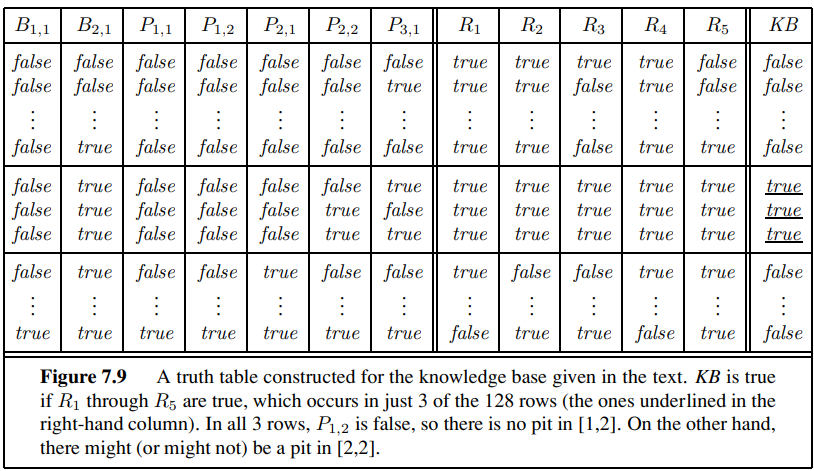
\includegraphics[]{images/wumpus-table.png}
\end{center}
Returning to our wumpus-world example, the relevant proposition \textbf{symbols} are $B_{1,1}, B_{2,1}, P_{1,1}, P_{1,2}, P_{2,1}, P_{2,2}$, and $P_{3,1}$. With seven symbols, there are $2^7 = 128$ possible models; in three of these, KB is true. Note that this is just a "snapshot" of the situation shown in the Figure 7.5. Obviously, as the agent goes on, the KB changes. In the three model where KB is \textit{True}, $\neg P_{1,2}$ is also \textit{True}. Hence, there is no pit in $[1,2]$. On the other hand, $P_{2,2}$ is true in two of the three models and false in one, so we cannot yet tell whether there is a pit in $[2,2]$. Note that KB is true if $R_1$ through $R_5$ are true (KB can be expressed as a sentence $R_1 \land ... \land R_5$), which occurs in just 3 of the 128 rows.
\begin{center}
    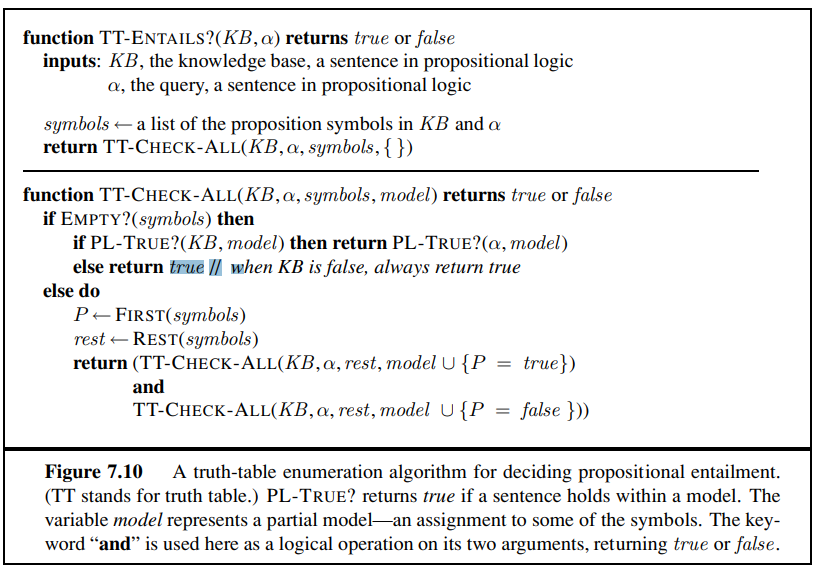
\includegraphics[]{images/tt-algorithm.png}
\end{center}
The algorithm above performs a recursive enumeration of a finite space of assignments to symbols. The algorithm is \textbf{sound} because it implements directly the definition of entailment, and \textbf{complete} because it works for any KB and $\alpha$ and always terminates; there are only finitely many models to examine.\newline\newline
Basically, the algorithm constructs the truth table seen above using a recursive implementation. In particular, it creates a binary tree where the nodes are the symbols in the KB and the branches are truth assignment for that symbol (\textit{True} or \textit{False}). It starts from the first symbol and recursively produces all the possible assignment for all the possible symbols. The paths from the root to the leaves corresponds to the rows of the table above, i.e. the models. Once the algorithm arrives at a leaf, it checks whether the sentence $\alpha$ holds within the corresponding model (path). The algorithm returns always \textit{True} if the KB is \textit{False} w.r.t the model because we are only interested to see if a sentence is \textit{True} when the KB is \textit{True}. These operations correspond to look at the rows of the table (models) where KB is \textit{True} and check whether $\alpha$ is also \textit{True}. If the sentence $\alpha$ is \textit{True} for all the models where also KB is \textit{True} (i.e. all the leaves \textit{returns} \textit{True}), then $\alpha$ can be deduces from KB. Note that if all the leaves return \textit{True}, when the algorithm ascents from recursion, the \textit{True} value is propagated towards the root by the logical \textit{and} and eventually the algorithm returns \textit{True}.  For the same reason, it is sufficient that just one leaf returns \textit{False} that the whole algorithm returns \textit{False} (this is why the algorithms always returns \textit{True} when KB is \textit{False}).\newline\newline
Note that If KB and $\alpha$ contain $n$ symbols in all, then there are $2^n$ models. Thus, the time complexity of the algorithm is $O(2^n)$ (The space complexity is only $O(n)$ because the enumeration is depth-first). Unfortunately, propositional entailment is co-NP-complete.

\chapter{Lec 09 - Neural Networks III}

\section{Other activation functions}
Multiple layers of cascaded units makes a Neural Network able to implement complex non linear functions. The non linearity of the model is given by the activation functions. In fact, without them (linear activation) the result of the model, even if it’s very complex, would still be linear. If we used step activation functions we wouldn't be able to resort to gradient descent to optimize the weights. This is because step function is not derivable. We have to choose one or more activation functions that are derivable.
\begin{itemize}
    \item \textbf{Sigmoid:}
    \[\sigma(y) = \frac{1}{1 + e^{-y}}\]

    \item \textbf{ReLu:}
    \[r(y) = max(0, y)\]
\end{itemize}
\section{Multi-layer Neural Networks: Keywords}
Let's define the most important keywords for Multi-layer Neural Networks:
\begin{itemize}
    \item $d$ \textbf{input units}: $d$ input data size $\textbf{x} \equiv (x_{1},...,x_{d})$, $d + 1$ when including the bias in the weight vector $\textbf{x}^{'} \equiv (x_{0}, x_{1},...,x_{d})$

    \item $n_{H}$ \textbf{hidden units} (with output $\textbf{y} \equiv (y_{1},...,y_{n_{H}})$)

    \item $c$ \textbf{output units}: $\textbf{z} \equiv (z_{1},...,z_{c})$. The number of desired output is $\textbf{t} \equiv (t_{1},...,t_{c})$

    \item $w_{ji}$ weight from the $i$-th input unit to the $j$-th hidden unit ($w_{j}$ is the weight vector of the $j$-th hidden unit)

    \item $w_{kj}$ weight from the $j$-th hidden unit to the $k$-th output unit ($w_{k}$ is the weight vector of the $k$-th output unit)
\end{itemize}
\section{Learning algorithm}
Let's consider, for example, a Neural Network with just one hidden layer and \textbf{sigmoid activation functions}. The basic idea of the learning algorithm consists in two phases:
\begin{itemize}
    \item \textbf{Forward phase:} for each example in the training set, present it to the network and compute the output.
    \item \textbf{Backward phase:} Back-propagate the committed error and update the weights of the hidden units accordingly. 
\end{itemize}
This algorithm is called \textbf{Backpropagation}\newline\newline
As we said before, this algorithm is based on gradient descent, so we need to minimize an error function $E[\textbf{w}]$ that can be defined as follows:
\[E[\textbf{w}] = \frac{1}{2cN}\sum_{s=1}^{N}\sum_{k=1}^{c}(t_{k}^{(s)} - z_{k}^{(s)})^{2}\]
In order to implement Backpropagation, we need to first compute the gradient for the weights of both output and hidden units.
\begin{itemize}
    \item \textbf{Gradient of the weights of an output unit:}
    \[\frac{\partial E}{\partial w_{\hat{k}\hat{j}}} = - \frac{1}{cN}\sum_{s=1}^{N}(t_{\hat{k}}^{(s)} - z_{\hat{k}}^{(s)} )z_{\hat{k}}(1 - z_{\hat{k}})y_{\hat{j}}^{(s)}\]
    where $y_{\hat{j}}^{(s)}$ is the output of the $\hat{j}$-th hidden unit.
    
    \item \textbf{Gradient of the weights of a hidden unit:}
    \[\frac{\partial E}{\partial w_{\hat{j}\hat{i}}} = - \frac{1}{cN}\sum_{s=1}^{N}y_{\hat{j}}^{(s)}(1 - y_{\hat{j}}^{(s)})x_{\hat{i}}^{(s)}\sum_{k=1}^{c}(t_{\hat{k}}^{(s)} - z_{\hat{k}}^{(s)} )z_{\hat{k}}(1 - z_{\hat{k}})w_{k\hat{j}}\]
\end{itemize}
Note that, for simplicity, we are considering a Neural Network with just one hidden layer, but the derivation can be extended for more than one hidden layer.
\subsection{Back-propagation algorithm}
Back-propagation is an algorithm that aims to update the weights of a Neural Network in order to minimize the error between the predicted output and the true output. The algorithm works by propagating the error back through the network, starting with the output layer and moving backwards through the hidden layers, adjusting the weights at each layer to reduce the error. It can be implemented in different ways:
\begin{itemize}
    \item \textbf{Batch gradient descent:} It \textbf{cumulates} gradients over all the training examples and then updates the weights.
    \item \textbf{Stochastic gradient descent:} For each example in $S$, it computes the gradients and update the weights.
    \item \textbf{Mini-batch gradient descent:} It updates the weights considering a subset of examples $Q \subseteq S$. 
\end{itemize}
This process is typically repeated many times until the error is sufficiently small or the maximum number of iterations is reached. Let's define the algorithm according to the derivations seen before:\newline\newline
\textbf{Back-propagation (stochastic)}
\begin{enumerate}
    \item Initialize all weights with small random values (e.g. between -0.5 and +0.5)
    \item Until the termination condition is satisfied:
    \begin{enumerate}
        \item For each $(\textbf{x},\textbf{t}) \in S$:
        \begin{enumerate}
            \item Present $\textbf{x}$ to the net and compute the vectors $\textbf{y}$ and $\textbf{z}$
            \item For each output unit $k$:
            \[\delta_{k} = z_{k}(1 - z_{k})(t_{k} - z_{k})\]
            \[\Delta w_{kj} = \delta_{k}y_{j}\]

            \item For each hidden unit $j$:
            \[\delta_{j} = y_{j}(1 - y_{j})\sum_{k=1}^{c}w_{kj}\delta_{k}\]
            \[\Delta w_{ji} = \delta_{j}x_{i}\]

            \item Update all weights:
            \[w_{sq} \leftarrow w_{sq} + \eta \Delta w_{sq}\]
        \end{enumerate}
    \end{enumerate}
\end{enumerate}
Note that this algorithm works only for a network with one hidden layer, but can be easily extended. In fact, the algorithm computes the error term $\delta$ for each unit of each layer, and then it multiplies this error term for the input of the unit.

\section{Computational power of neural networks}
\textbf{Theorem (Pinkus, 1996) simplified}:\newline
Given a feed-forward NN with just one hiddel layer, any continuous function $f:\mathbb{R}^{n} \rightarrow \mathbb{R}$ and an arbitrarily small $\epsilon > 0$, then, for a large class of activation functions, there always exists an integer $M$ such that the function $g: \mathbb{R}^{n} \rightarrow \mathbb{R}$ computed by the net using at least $M$ hidden units approximates the function $f$ with tolerance $\epsilon$, that is:
\[max_{x \in \Omega}|f(\textbf{x}) - g(\textbf{x})| < \epsilon\]
Note that the theorem attests the existence of a NN with $M$ hidden units that approximates the target function with the desired tolerance, but it says nothing about how $M$ can be computed.

\section{Fine tuning neural networks}
The choice of the net typology determines the hypothesis space used. With three-layers architecture (input, hidden, output), the number of hidden units detrmines the complexity of the hypothesis space. As we said for the Perceptron, the choice of the learning rate $\eta$ can be crucial for the convergence.
\subsection{Avoiding local minima}
The local minima problem in neural networks refers to the scenario where a neural network gets stuck in a sub-optimal solution during the training process. Instead of reaching the global minimum, which is the best possible solution, the network settles for a local minimum, that may not be the best fit for the data. This can happen because the loss function used can have multiple local minima, and the optimization algorithm may only find one of them. In order to avoid this problem, we can use different techniques:
\begin{itemize}
    \item Adding a term to the weight update rule (called \textbf{momentum}). Basically, a contribution deriving from the previous step is added, imposing a kind of inertia on the system.

    \item Using \textbf{stochastic training} (randomizing on the examples) instead of batch training can facilitate to avoid local minima.

    \item \textbf{Training multiple NNs} on the same data with different initialization and combining the outputs.
\end{itemize}

\subsection{Over-fitting}
With neural networks, usually, the error on the validation set increases as the number of weight updates increases. This is because, at the beginning, with small absolute values of the weights (similar each other), the decision surfaces are \textit{smoother}. When the absolute values of the weights increase , the complexity of the decision surfaces increases and with it the possibility to suffer over-fitting. \newline\newline
A possible solution can be to use an additional term in the error function to minimize based on the norm of the weights (regularization) $E + ||w||^{2}$.

\section{Hidden layer representation}
An important feature of multi-layer NNs is that they can find useful representations of input data (alternative to the input representation). Specifically, the output of the hidden units is an effective new input representation for the next layers. This feature can be used to define a particular type of NNs called Auto-encoders.


\chapter{Lec 10 - Generalized Linear Models and SVM I}
\section{Linear Models}
Linear models are one of the most important types of models in machine learning. A linear model is of the form:
\[f_{\textbf{w},b}(\textbf{x}) = \sum_{i=1}^{m} w_{i}x_{i} + b = \textbf{w} \cdot \textbf{x} + b\]
Which can also be written as
\[f_{\textbf{w},b}(\textbf{x}) = \sum_{i=0}^{m} w_{i}x_{i}= \textbf{w} \cdot \textbf{x}\]
where $x_{0} = 1$.
\begin{itemize}
    \item For \textbf{classification}, the sign of the result is returned, that is:
    \[h(\textbf{x}) = sign(f_{\textbf{w}}) \in \{-1, +1\}\]

    \item For \textbf{regression}, the \textit{original} function can be taken, that is:
    \[h(\textbf{x}) = f_{\textbf{w}} \in \mathbb{R}\]
\end{itemize}
\subsection{Linear Regression}
Given a training set $S = \{(\textbf{x}_{1}, y_{1}), ..., (\textbf{x}_{n}, y_{n})\}$, in linear regression we look for a hypothesis $h_{\textbf{w}}$ which minimizes the mean squared error on the training set, that is:
\[argmin_{\textbf{w}} \frac{1}{n}\sum_{i=0}^{n}(h_{\textbf{w}}(\textbf{x}_{i}) - y_{i})^{2}\]
We can formalize it in matrices terms:
\[E(\textbf{w}) = \frac{1}{n}\sum_{i=0}^{n}(h_{\textbf{w}}(\textbf{x}_{i}) - y_{i})^{2}\]
\[= \frac{1}{n}\sum_{i=0}^{n}(\textbf{w} \cdot \textbf{x}_{i} - y_{i})^{2}\]
\[= \frac{1}{n}||\textbf{Xw} - \textbf{y}||\]
where:
\begin{itemize}
    \item $\textbf{X}$ is a matrix of size $n \times d$
    \item $\textbf{w}$ is a vector of size $d \times 1$
    \item $\textbf{y}$ is a vector of size $n \times 1$
\end{itemize}
$d$ is the dimension of the feature space (including the bias term). Basically, we want that $\textbf{Xw} \approx \textbf{y}$.\newline\newline
Since $||\vec{z}||^{2} = \sum_{i}z_{i}^{2}$, the optimization problem can be defined as follows:
\[min_{\textbf{w}}E(\textbf{w}) \equiv \frac{1}{n}||\textbf{Xw} - \textbf{y}||^{2}\]
We want to find the vector $\textbf{w}$ that minimizes $E$. Basically, we want to find the points $\textbf{w}$ where the gradient vanishes (equals to 0), that is:
\[\nabla E(\textbf{w}) = \frac{2}{n}\textbf{X}^{T} (\textbf{Xw} - \textbf{y}) = 0\]
\[\textbf{X}^{T}\textbf{Xw} = \textbf{X}^{T}\textbf{y}\]
By multiplying the quantity $(\textbf{X}^{T}\textbf{X})^{-1}$ both on the left and on the right of the equation, it becomes:
\[(\textbf{X}^{T}\textbf{X})^{-1}(\textbf{X}^{T}\textbf{X})\textbf{w} = (\textbf{X}^{T}\textbf{X})^{-1}\textbf{X}^{T}\textbf{y}\]
Since $(\textbf{X}^{T}\textbf{X})^{-1}(\textbf{X}^{T}\textbf{X})$ is the identity matrix, the final equation is:
\[\textbf{w} = (\textbf{X}^{T}\textbf{X})^{-1}\textbf{X}^{T}\textbf{y}\]
This is a \textbf{closed form solution}. It means that with just one computation we are able to find the solution, it's not am iterative process. However, computing the inverse of a matrix can be very computational inefficient.

\subsection{Non-linear mapping}
The goal of non-linear mapping is to apply a transformation to non-linearly separable points in order to map them in a new feature space that is linearly separable. Then, a linear model (hyperplane) in the transformed space will correspond to a non-linear decision surface in the original space (Generalized Linear Models).

\section{Linear separability}
Consider the hypothesis space of hyperplanes. Given a set of linearly separable points, we have different hyperplanes that separates them. Intuitively, the widest possible margin (or \textbf{optimal}) hyperplane is the best one, because is the one that generalizes better, but how can we compute to which $\textbf{w}$, $b$ the best hyperplane corresponds.
\subsection{Margin of a hyperplane}
The margin of a hyperplane is the distance between the hyperplane and the closest data points of each class. \newline\newline
Let's consider the \textbf{binary classification} problem. Given the hyperplane $\textbf{w} \cdot \textbf{x} + b = 0$ (\textbf{optimal hyperplane}), the \textit{"distance"} of a point $\textbf{x}$ from the hyperplane can be expressed by the algebraic measure $g(\textbf{x}) = \textbf{w}^{T} \cdot \textbf{x} + b$. We can write $\textbf{x}$ as follows:
\[\textbf{x} = \textbf{x}_{p} + r\frac{\textbf{w}}{||\textbf{w}||}\]
where:
\begin{itemize}
    \item $||\textbf{w}||$ is the norm of $\textbf{w}$
    \item $\textbf{x}_{p}$ is the normal projection of $\textbf{x}$ onto the hyperplane.
    \item $r$ is the desired algebraic distance ($r > 0$ if $\textbf{x}$ is on the positive side of the hyperplane, otherwise $r < 0$).
\end{itemize}
Note that $g(\textbf{x}_{p}) = 0$ because $\textbf{x}_{p}$ is on the hyperplane. Furthermore, since we are considering the optimal hyperplane, the absolute distance between this hyperplane and any nearest positive example is the same as the absolute distance between any negative example. So, we can \textit{normalize} the value of $g$ such that $g(\textbf{x}) = 1$ if $\textbf{x}$ is in the positive margin hyperplane and $g(\textbf{x}) = -1$ if $\textbf{x}$ is in the negative margin hyperplane.\newline\newline
Take $\textbf{x}_{k}$ in the positive margin hyperplane, it follows that
\[g(\textbf{x}_{k}) = \textbf{w}^{T}\textbf{x}_{k} + b\]
Since $\textbf{x}_{k} = \textbf{x}_{p} + r\frac{\textbf{w}}{||\textbf{w}||}$:
\[= \textbf{w}^{T}\left(\textbf{x}_{p} + r\frac{\textbf{w}}{||\textbf{w}||}\right) + b\]
\[= \textbf{w}^{T}\textbf{x}_{p} + b + r\frac{\textbf{w}^{T}\textbf{w}}{||\textbf{w}||}\]
Since $\textbf{w}^{T}\textbf{w} = ||\textbf{w}||^{2}$:
\[= \textbf{w}^{T}\textbf{x}_{p} + b + r||\textbf{w}||\]
The term $\textbf{w}^{T}\textbf{x}_{p} + b = 0$ because, as we said before, $g(\textbf{x}_{p}) = 0$. This implies that:
\[g(\textbf{x}_{k}) = r||\textbf{w}|| = +1\]
This is true only if
\[r = \frac{1}{||\textbf{w}||}\]
Then, the margin $\rho$ is defined as follows:
\[\rho = 2r = \frac{2}{||\textbf{w}||}\]
\section{Support Vector Machines (SVM)}
Support Vector Machines (SVMs) are a set of supervised learning methods used for classification and regression tasks. The idea behind SVMs is to find the best hyperplane that separates the training data. This hyperplane is chosen in such a way that it maximizes the margin.
\subsection{Separable case: Quadratic optimization}
If we have $n$ linearly separable examples $\{(\textbf{x}_{i}, y_{i})\}$ (binary classification), it is possible to find the optimal hyperplane $h(\textbf{x}) = sign(\textbf{w} \cdot \textbf{x} + b)$ by solving the following \textbf{constrained} quadratic optimization problem:
\[min_{\textbf{w},b}\frac{1}{2}||\textbf{w}||^{2}\]
\[subject \,\, to: \,\, \forall i \in \{1,...,n\}: y_{i}(\textbf{w} \cdot \textbf{x}_{i} + b) \geq 1\]
Since the margin is defined as $\rho = \frac{2}{||\textbf{w}||}$ and we want to maximize it, we need to minimize $||\textbf{w}||$. This minimization problem is subject to the constraint that each point in the training set must be on the \textit{correct} side of the hyperplane, which means that for each point, the following inequality must hold: $\forall i \in \{1,...,n\}: y_{i}(\textbf{w} \cdot \textbf{x}_{i} + b) \geq 1$. This constraint is given by the fact that:
\begin{itemize}
    \item $\textbf{w} \cdot \textbf{x}_{i} + b \geq 1$ if $y_{i} = +1$
    \item $\textbf{w} \cdot \textbf{x}_{i} + b \leq 1$ if $y_{i} = -1$
\end{itemize}
This is a \textbf{convex} constrained quadratic problem, and for this reason it guarantees a unique solution.\newline\newline
With a large number of features it can be computationally inefficient to solve this problem, so we can use its \textbf{dual formulation}
\subsection{Dual formulation}
In the dual problem, Lagrange multipliers $\alpha_{i} \geq 0$ are associated with every constraint in the primal problem (one for each example).
\[max_{\alpha} \sum_{i=1}^{n}\alpha_{i} - \frac{1}{2}\sum_{i,j=1}^{n}y_{i}y_{j}\alpha_{i}\alpha_{j}(\textbf{x}_{i} \cdot \textbf{x}_{j})\]
\[subject \,\, to: \,\, \forall i \in \{1,...,n\}: \,\, \alpha_{i} \geq 0 \,\, and \,\, \sum_{i=1}^{n}y_{i}\alpha_{i} = 0\]
At the solution, most of the $\alpha_{i}$'s are zeros. Those examples associated with non zero multipliers are called \textbf{support vectors}.

\subsection{SVM solution}
The primal solution turns out to be:
\[\textbf{w} = \sum_{i=1}^{n}y_{i}\alpha_{i}\textbf{x}_{i}\]
\[b = y_{k} - \textbf{w} \cdot \textbf{x}_{k}\,\, \forall \textbf{x}_{k}\,\,s.t\,\, \alpha_{k} > 0\]
Hence:
\[h(\textbf{x}) = sign(\textbf{w} \cdot \textbf{x} + b) = sign\left(\sum_{i = 1 \in support \,\, vector}^{n}y_{i}\alpha_{i}(\textbf{x}_{i} \cdot \textbf{x}) + b\right)\]
The decision function only depends on dot products between the point and othe points in the training set (the support vectors).

\chapter{Lec 11 - NP-Hardness}

\section{Tractable vs Intractable problems}
Problems for which a polynomial algorithm exists are called \textbf{tractable}. If no such algorithm exists, the problem is called \textbf{intractable}.\newline\newline
\textbf{Examples:}
\begin{enumerate}
    \item \textbf{Eulerian circuit problem:} Given an undirected graph, an Eulerian circuit is a cycle that traverses all the edges only once. This problem can be solved in linear time. Note that in an Euler circuit you might pass through a vertex more than once.

    \item \textbf{Hamiltonian circuit problem:} Given an undirected graph, an Hamiltonian circuit is a cycle that traverses all the vertices only once. To date, no one knows a polynomial algorithm to solve it. Note that in a Hamiltonian circuit you may not pass through all edges.

    \item \textbf{Minimum spanning tree:}

    \item \textbf{Traveling Salesperson Problem (TSP):} Given a complete, undirected graph and a function $w: E \rightarrow \mathbb{R}$, output a \textbf{tour} (i.e. a cycle that visits every vertex exactly once) of minimum cost
    \[T \subseteq E \quad \text{minimizing }\sum_{e \in T}w(e)\]
    To date, no one knows a polynomial algorithm to solve it.
\end{enumerate}
A much easier task can be the following: Given a graph and a list of vertices $C$, \textbf{check} if $C$ is an Hamiltonian circuit.\newline\newline
Problems that are \textit{easy} to solve belong to the \textbf{complexity class} \textbf{P} (\textit{polynomial time}), 1), 3) $\in$ \textbf{P}. Problems that are \textit{easy} to verify belong to the complexity class \textbf{NP} (\textit{Non-deterministic polynomial}), 1), 2) ,3) ,4) $\in$ \textbf{NP}.

\section{NP-Hard}
\textbf{Decision Problems:}\newline
To simplify the study of the complexity of problems, we limit our attention to problems with a boolean answer (YES, NO), that is, decision problems.\newline\newline
Let's define \textbf{P} and \textbf{NP} classes in a more formal way:
\begin{itemize}
    \item \textbf{P} is the set of decision problems that can be solved in polynomial time.

    \item \textbf{NP} is the set of decision problems with the following property: if the answer is YES, then there is a proof of this fact that can be checked in polynomial time.

    \item \textbf{NP-Hard:} A computational problem is \textbf{NP-Hard} if a polynomial-time algorithm that solves it would imply a polynomial-time algorithm that solves every problem in \textbf{NP}.\newline\newline
    A problem is \textbf{NP-Complete} if it is both in \textbf{NP} and \textbf{NP-Hard}. Basically, these problems are the hardest in \textbf{NP}. 
\end{itemize}
\begin{figure}[h]
    \centering
    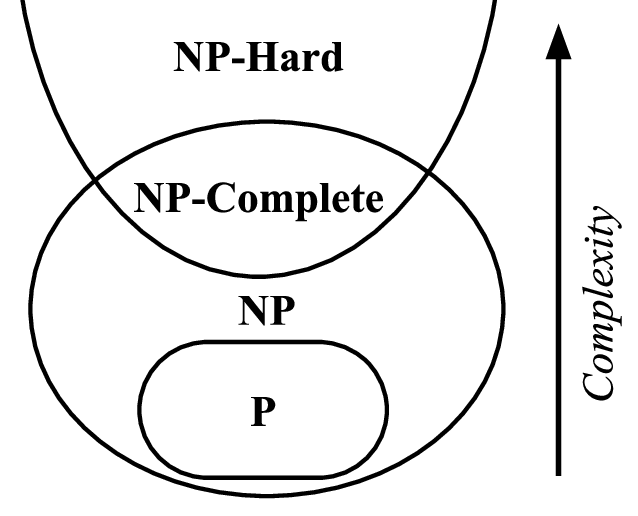
\includegraphics[scale=0.4]{images/P-NP.png}
    \caption{What we think the computation classes look like}
    \label{fig:P-NP-Np-Hard}
\end{figure}
One of the main open questions in computer science is whether \textbf{P=NP}.\newline\newline
Studying NP-Hardness is important because if a problem is \textbf{NP-Hard} is a strong evidence that it is intractable. It suggests you to use a different approach, such as identify tractable special-cases, or use \textbf{approximation algorithms}.

\section{Cook-Levin Theorem}
\textit{In computational complexity theory, the Cook–Levin theorem, also known as Cook's theorem, states that the Boolean satisfiability problem is \textbf{NP-complete}.}\footnote{Wikipedia definition}\newline\newline
SAT: formula satisfiability:
\begin{itemize}
    \item input: A boolean formula like the following: $(b \land \neg c) \lor (\neg a \land b)$

    \item output: It is possible to assign boolean values to the variables $a, b, c, ...$ such that the entire formula evaluates to TRUE?
\end{itemize}
determining the satisfiability of a formula in conjunctive normal form (CNF) where each clause is limited to at most three literals is \textbf{NP-complete} also; this problem is called \textbf{3-SAT}.\newline\newline
\textbf{Example of 3-CNF formula:}
\[(a \lor b \lor c) \land (b \lor \neg c \lor \neg d) \land (\neg a \lor c \lor d)\]
%Check if the theorem was defined on 3SAT???
How can we show that a problem is \textbf{NP-Hard}?

\section{Reductions}

To prove that a problem $P$ is \textbf{NP-Hard} we use \textbf{reduction}. We want to prove that every problem in \textbf{NP} reduces to problem $P$.\newline\newline
Reducing problem $A$ to problem $B$ means describing an algorithm to solve $A$ under the assumption that an algorithm for $B$ exists.
\begin{center}
    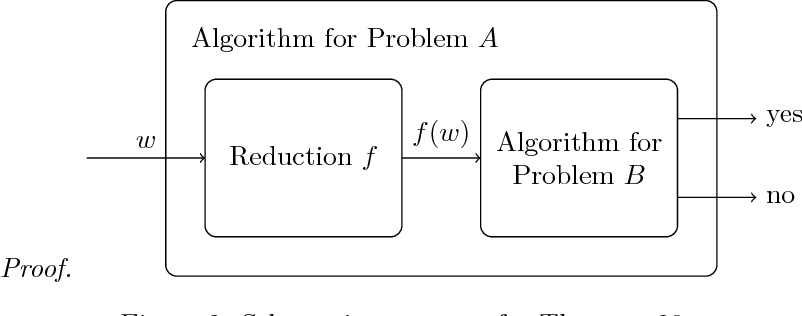
\includegraphics[scale=0.4]{images/Reduction.png}
\end{center}
$A < B$ means \textit{A reduces to B} where $B$ is the hardest problem ($A$ is as hard as $B$).


\chapter{Lec 12 - Preprocessing}

\section{Supervised learning pipeline}
The supervised learning pipeline can be summarized as follows:
\begin{enumerate}
    \item Analysis of the problem (Classification, Regression, ...)

    \item Collection, analysis and cleaning data

    \item Pre-processing and managing missing values

    \item Study of correlation between variables 

    \item Feature selection/weighting/learning

    \item Choice of the predictor and model selection

    \item Test
\end{enumerate}
Some of the most common objects that we can find in machine learning are:
\begin{itemize}
    \item \textbf{Vectors} (Set of values)
    \item \textbf{Strings}
    \item \textbf{Sets and Bags}: for example, the set of terms in a document or their frequency
    \item \textbf{Tensors}: for example, images and video
    \item \textbf{Trees and graphs}
\end{itemize}
The easiest way to represent these objects is to map them in a vectorial representation.\newline\newline
Features values can be divided in two classes: \textbf{Categorical} and \textbf{Quantitative}:
\begin{itemize}
    \item Categorical or symbolic features
    \begin{itemize}
        \item Nominals: They are used for naming or labeling variables, without any quantitative value. There is usually no intrinsic ordering to nominal data.

        \item Ordinals: Is a type of categorical data with an order.
    \end{itemize}

    \item Quantitative and numeric features:
    \begin{itemize}
        \item Intervals (Enumerables)
        \item Ration (Real values)
    \end{itemize}
\end{itemize}
Let's see how to encode categorical and quantitative variables into a vector.

\section{Encoding categorical or symbolic variables}
One of the most common method to encode a categorical variable into a vector is the \textbf{OneHot Encoding}. This technique allows you to represents categorical variables in a vector with as many components as the number of possible values for the variable.\newline\newline
For example, let's say that we want to encode a variable corresponding to the brand of a car. The possible values that an instance can take are: \textit{(Fiat, Toyota, Ford)}. The OneHot encoding of an instance having \textit{Toyota} as brand value could be the following: $[0, 1, 0]$. Basically, it's a vector where we set to one the component corresponding to the value of the instance.

\section{Encoding of continuous variables}
In this case, it is more difficult to find a good mapping. Therefore, the features are typically transformed to obtain values \textit{comparable} with other features.\newline\newline
Given a matrix of instances (training set), for each feature $j$, let $\hat{x}_{j} = \frac{1}{n}\sum_{i=1}^{n}x_{ij}$ be the average value of the current feature and let $\sigma_{j} = \sqrt{\frac{1}{n}\sum_{i=1}^{n}(x_{ij} - \hat{x}_{j})^{2}}$ be the standard deviation of $j$. We can apply the following transformations:
\begin{itemize}
    \item Centering: $c(x_{ij}) = x_{ij} - \hat{x}_{j}$. For each value $x_{ij}$ we compute $c(x_{ij})$ which is equal to the difference between the value and the average of the corresponding feature.

    \item Standardization: $s(x_{ij}) = \frac{c(x_{ij})}{\sigma_{j}}$. We want the \textit{columns} (features) of the matrix to have mean equals to 0 and variance equals to 1.

    \item Scaling to a range: $h(x_{ij}) = \frac{x_{ij} - x_{min j}}{x_{max j} - x_{min j}}$. Each value is scaled in a range between 0 and 1.

    \item Normalization: $g(\textbf{x}) = \frac{\textbf{x}}{||\textbf{x}||}$. In this case, we don't work over features but we want to normalize the instances (rows).
\end{itemize}
The python module \textit{sklearn} provides several methods to perform this kind of pre-processing.

\subsection{K-Nearest Neighbors}
K-Nearest Neighbors is a simple classification algorithm where a test example is classified with the majority class of its k-neighbors in the training set.\newline\newline
When the instances are \textbf{normalized} we can define the squared distance between them in terms of dot-product:
\[||\textbf{x} - \textbf{z}||^{2}\]
\[= ||\textbf{x}||^{2} + ||\textbf{z}||^{2} - 2\langle \textbf{x}, \textbf{z}  \rangle\]
Since the norm of the instances is equal to 1, it follows that:
\[= 2 - 2\langle \textbf{x}, \textbf{z}  \rangle\]
So, with normalized data, the distance between two instances is inversely proportional to their dot-product.

\section{Feature selection and feature extraction}
Feature \textbf{selection} is the reduction of the dimensionality of the features obtained by removing irrelevant or redundant features. The interpretability of the model is maintained.\newline\newline
Feature \textbf{extraction} is the reduction of the dimensionality of the features obtained by combining the original features (e.g. PCA). Generally, the interpretability of the model is lost.

\subsection{Feature selection}
The top reasons to use feature selection are:
\begin{itemize}
    \item It enables the machine learning algorithm to train faster

    \item It reduces the complexity of a model and makes it easier to interpret.

    \item It improves the accuracy of a model if the right subset is chosen.

    \item It reduces over-fitting.
\end{itemize}
Feature selection methods can be divided in 3 classes:
\begin{itemize}
    \item \textbf{Filter methods:} They perform feature selection before applying the predictor. They use an efficient scoring function (e.g. Mutual information, Chi squared, Information gain) that determines the usefulness of a given set of features.

    \item \textbf{Wrapped methods:} The predictor is evaluated on a hold-out sample using subset of different features. Then, the subset with highest score is chosen.

    \item \textbf{Embedded methods:} The selection of features occurs in conjunction with the training of the model, for example, by modifying the objective function to be optimized. 
\end{itemize}

\subsection{Feature extraction (PCA)}
\textbf{Principal Component Analysis (PCA)} converts a set of instances with possibly related features into corresponding values on another set of linearly unrelated features (principal components).\newline\newline
\textbf{Neural Networks} can also be seen as a particular way to perform feature extraction on their hidden layers. In fact, the output values of one of the hidden layers can be considered as a new representation of the original data.


\chapter{Lec 13 - Resolution for First Order Logic}

\section{Resolution}
The last of our three families of logical systems is based on \textbf{resolution}. In resolution for first order logic two clauses, which are assumed to be standardized apart so
that they share no variables, can be resolved if they contain complementary literals. Propositional literals are complementary if one is the negation of the other; first-order literals are complementary if one unifies with the negation of the other. Thus, we have
\begin{center}
    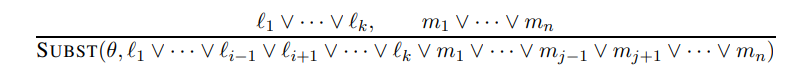
\includegraphics[]{images/resolution-fol.png}
\end{center}
where $UNIFY(l_i,\neg{m_j} ) = \theta$. For example, we can resolve the two clauses
\[[Animal(F(x)) \lor Loves(G(x), x)]\,\, \text{and} \,\,[\neg Loves(u, v) \lor \neg Kills(u, v)]\]
by eliminating the complementary literals $Loves(G(x), x)$ and $\neg Loves(u, v)$, with unifier $\theta = \{u/G(x), v/x\}$, to produce the \textbf{resolvent} clause
\[[Animal(F(x)) \lor \neg Kills(G(x), x)] .
\]
Then, the resolution steps can be applied to $CNF(KB \land \neg \alpha)$ as we did for propositional logic.

\section{Conversion to CNF}
As in the propositional case, first-order resolution requires that sentences be in \textbf{conjunctive
normal form} (CNF), that is, a conjunction of clauses, where each clause is a disjunction of literals. Literals can contain variables, which are assumed to be universally quantified. Every sentence of first-order logic can be converted into an inferentially equivalent CNF
sentence.\\\\
We illustrate the procedure by translating the sentence “Everyone who loves all animals is loved by someone,” or
\[\forall x \, [\forall y \, Animal(y) \Rightarrow Loves(x, y)] \Rightarrow [\exists y \, Loves(y, x)].\]
The steps are as follows:
\begin{itemize}
    \item \textbf{Eliminate implications:}
    \[\forall x \, [\neg \forall y \, \neg Animal(y) \lor Loves(x, y)] \lor [\exists y \, Loves(y, x)] .\]

    \item \textbf{Move} $\neg$ \textbf{inwards}: In addition to the usual rules for negated connectives, we need rules for negated quantifiers. Thus, we have
    \[\begin{split}
        & \neg \forall x \, p \,\, \text{becomes} \,\, \exists x \, \neg p\\
        & \neg \exists x \, p \,\, \text{becomes} \,\, \forall x \, \neg p .
    \end{split}\]
    Our sentence goes through the following transformations:
    \[\begin{split}
        & \forall x \, [\exists y \, \neg(\neg Animal(y) \lor Loves(x, y))] \lor [\exists y \, Loves(y, x)].\\
        & \forall x \,[\exists y \, \neg \neg Animal(y) \land \neg Loves(x, y)] \lor [\exists y \, Loves(y, x)].\\
        & \forall x \,[\exists y \, Animal(y) \land \neg Loves(x, y)] \lor [\exists y \, Loves(y, x)]
    \end{split}
    \]

    \item \textbf{Standardize variables}: each quantifier should use a different one:
    \[\forall x \,[\exists y \, Animal(y) \land \neg Loves(x, y)] \lor [\exists z \, Loves(z, x)] .\]

    \item \textbf{Skolemize:} \textbf{Skolemization} is the process of removing existential quantifiers by elimination. In the simple case, it is just like the Existential Instantiation rule seen previously: translate $\exists x \, P(x)$ into $P(A)$, where $A$ is a new constant. However, we can’t apply Existential Instantiation to our sentence above. If we blindly apply the rule to the two matching parts we get
    \[\forall x \, [Animal(A) \land \neg Loves(x, A)] \lor Loves(B,x),\]
    which has the wrong meaning entirely: it says that everyone either fails to love a particular animal $A$ or is loved by some particular entity $B$. Thus, we want the Skolem entities to depend on $x$ and $z$:
    \[\forall x \, [Animal(F(x)) \land \neg Loves(x, F(x))] \lor Loves(G(z), x) .\]
    Here $F$ and $G$ are \textbf{Skolem functions}.  The general rule is that the arguments of the Skolem function are all the universally quantified variables in whose scope the existential quantifier appears.

    \item \textbf{Drop universal quantifiers:}  At this point, all remaining variables must be universally quantified. Moreover, the sentence is equivalent to one in which all the universal quantifiers have been moved to the left. We can therefore drop the universal quantifiers:
    \[[Animal(F(x)) \land \neg Loves(x, F(x))] \lor Loves(G(z), x) .\]


    \item \textbf{Distribute} $\lor$ \textbf{over} $\land$:
    \[[Animal(F(x)) \lor Loves(G(z), x)] \land [\neg Loves(x, F(x)) \lor Loves(G(z), x)].\]
\end{itemize}
The sentence is now in CNF and consists of two clauses.

\section{Example proofs}
Resolution proves that $KB \vDash \alpha$ by proving $KB \land \neg \alpha$ unsatisfiable, that is, by deriving the empty clause. The algorithmic approach is identical to the propositional case. We give two example proofs. The first is the crime example presented in the previous sections. The sentences in CNF are:
\begin{center}
    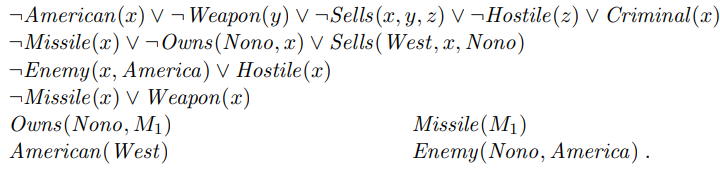
\includegraphics[]{images/crime-cnf.png}
    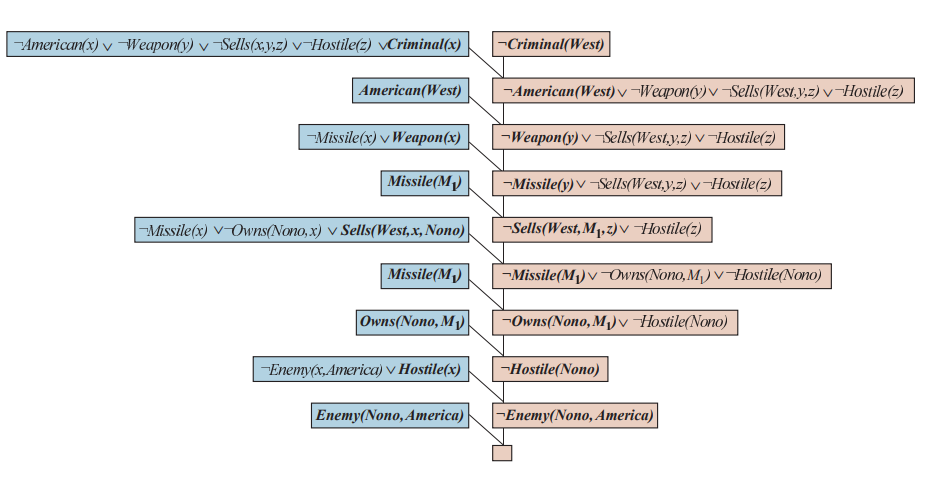
\includegraphics[]{images/resolution-crime-fol.png}
\end{center}
The resolution proof is shown in the figure above. Notice the structure: single “spine” beginning with the goal clause, resolving against clauses from the knowledge base until the empty clause is generated. This is characteristic
of resolution on Horn clause knowledge bases. In fact, the clauses along the main spine correspond exactly to the consecutive values of the goals variable in the backward-chaining algorithm.\\\\
Our second example makes use of Skolemization and involves clauses that are not definite clauses. This results in a somewhat more complex proof structure. In English, the problem is as follows:
\begin{center}
    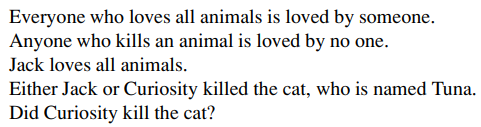
\includegraphics[]{images/resolution-fol-proof.png}
\end{center}
First, we express the original sentences, some background knowledge, and the negated goal G in first-order logic:
\begin{center}
    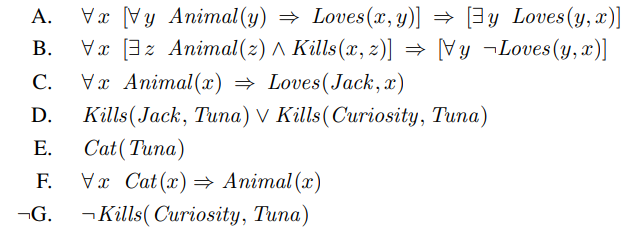
\includegraphics[]{images/kb-res-proof.png}
\end{center}
Now we apply the conversion procedure to convert each sentence to CNF:
\begin{center}
    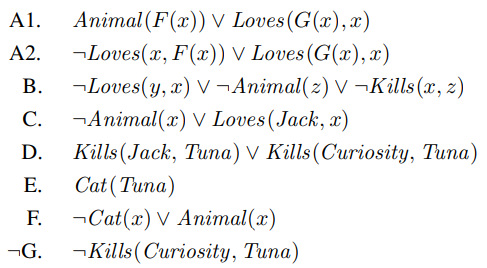
\includegraphics[]{images/kb-cnf-re-prrof.png}
\end{center}
The resolution proof that Curiosity killed the cat is given in the figure below:
\begin{center}
    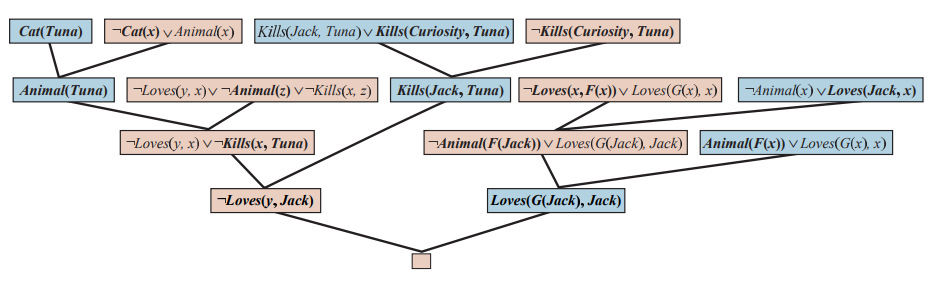
\includegraphics[]{images/res-proof-tree.png}
\end{center}
The proof answers the question “Did Curiosity kill the cat?” but often we want to pose more general questions, such as “Who killed the cat?”. Then, the goal is $\exists w \, Kills(w, Tuna)$, which, when negated, becomes $\neg Kills(w, Tuna)$ in CNF. Repeating the proof with the new negated goal, we obtain a similar proof tree, but with the substitution {w/Curiosity} in one of the steps. Unfortunately, resolution can produce \textbf{nonconstructive proofs} for existential goals. For example, $\neg Kills(w, Tuna)$ resolves with $Kills(Jack, Tuna) \lor Kills(Curiosity, Tuna)$ to give $Kills(Jack, Tuna)$, which resolves again with $\neg Kills(w, Tuna)$ to yield the empty clause. Notice that $w$ has two different bindings in this proof; resolution is telling us that, yes, someone killed Tuna, either Jack or Curiosity. This is no great surprise!
\begin{center}
    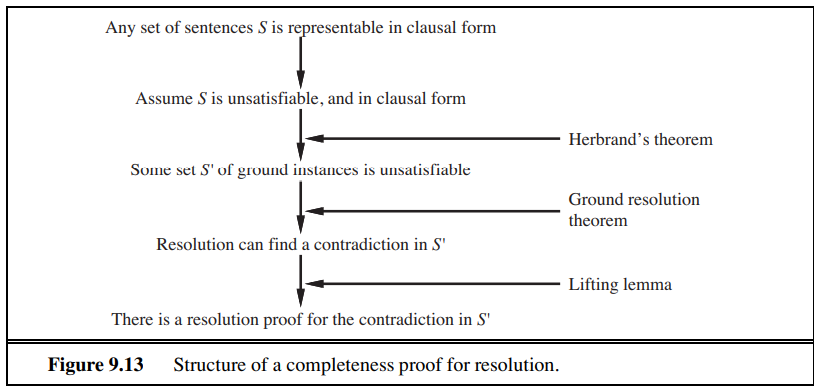
\includegraphics[]{images/res-completeness-fol.png}
\end{center}

\section{Resolution strategies}
We know that repeated applications of the resolution inference rule will eventually find a proof if one exists. In this subsection, we examine strategies that help find proofs efficiently.
\begin{itemize}
    \item \textbf{Unit preference/clause}: prefers to do resolutions where one of the sentences is a single literal.  The idea behind the strategy is that we are trying to produce an empty clause, so it might be a good idea to prefer inferences that produce shorter clauses.

    \item \textbf{Unit resolution:} is a restricted form of resolution in which every resolution step \textbf{must} involve a unit clause. Unit resolution is incomplete in general, but complete for Horn clauses. Unit resolution proofs on Horn clauses resemble forward chaining.

    \item \textbf{Set of support:} every resolution step involve at least one element of a special set of clauses (the set of support); the resolvent is then added into the set of support. Incomplete if the wrong set of support is chosen.

    \item \textbf{Input resolution:} In this strategy, every resolution combines one of the input sentences (from the KB or the query) with some other sentence. Complete for knowledge bases that are in Horn form, but incomplete in the general case. Input resolution has the characteristic shape of a single “spine” with single sentences combining onto the spine. The \textbf{linear resolution} strategy is a slight generalization that allows $P$ and $Q$ to be resolved together either if $P$ is in the original KB or if $P$ is an ancestor of $Q$ in the proof tree. Linear resolution is complete.

    \item \textbf{Subsumption:} eliminates all sentences that are subsumed by (that is, more specific than) an existing sentence in the KB. For example, if $P(x)$ is in the KB, then there is no sense in adding $P(A)$ and even less sense in adding $P(A) \lor Q(B)$. Subsumption helps keep the KB small and thus helps keep the search space small.

\end{itemize}

\chapter{Lec 14 - Higher-order functions for trees III}

\section{Trees type definition}
Until now we used binary trees that support data only in the leaves. Let's change the type definition in order to support information attached to nodes. We can do this in many different ways:
\begin{lstlisting}[style = FSharpStyle]
    type 'a tree =
        | Node of 'a * 'a tree * 'a tree
        | Leaf of 'a
\end{lstlisting}
In this case, a node is composed by an element of type 'a (which is the information attached to it) and the two sub-trees. However, with this definition we wouldn't be able to represent dead branches. In fact, each node must always have two sub-trees that can be either another node or a leaf.
\begin{lstlisting}[style = FSharpStyle]
    type 'a tree =
        | Node of 'a * 'a tree * 'a tree
        | Leaf of 'a option
\end{lstlisting}
With this implementation we can represent a dead branch defining a Leaf of None, but we could even define nodes with two empty leaves. So, this definition allows the programmer to write things that are not in their most simplified form.\newline\newline
In order to prevent this, we can do the following:
\begin{lstlisting}[style = FSharpStyle]
    type 'a tree =
        | Node of 'a * 'a tree option * 'a tree option
\end{lstlisting}
Now the \textbf{Node} data-constructor is a triple composed by:
\begin{itemize}
    \item An element of type 'a (information in the node)
    \item Two 'a tree option elements which represent the left and right sub-trees
\end{itemize}
When both the sub-trees are None, we are representing a leaf.\newline\newline
Let's write in F\# the following tree using this definition:\newline
\begin{tikzpicture}
    \Tree
    [.5  
        [.6
            \edge[]; {1}
            \edge[]; {2}
        ]
        [.7
            \edge[]; {3}
            \edge[blank]; \node[blank]{};
        ]
    ]
\end{tikzpicture}\newline
\begin{lstlisting}[style = FSharpStyle]
    let Leaf x = Some(Node(x, None, None))
    let tree = Node(5,
                Some(Node(6, Leaf 1, Leaf 2)),
                Some(Node(7, Leaf 3, None)))
\end{lstlisting}
Note that \textbf{Leaf x} is a function, not a data-constructor. It is just a shorter way to define leaves. The difference between functions and data-constructors is that functions can be used to \textbf{create}, but not for deconstructing (they can't be used to pattern-match).\newline\newline
We can write trees even in a shorter form by defining the following function:
\begin{lstlisting}[style = FSharpStyle]
    let SNode (x, t1, t2) = Some (Node (x, t1, t2))
    let tree = Node (5, 
               SNode (6, Leaf 1, Leaf 2), 
               SNode (7, Leaf 3, None)
               )
\end{lstlisting}
How can we pattern-match this type definition ? We have to specify all possible combinations of node types.
\begin{lstlisting}[style = FSharpStyle]
    let rec pretty_tree t = 
        match t with
        | Node(x, None, None) -> sprintf "(. %O .)" x
        | Node(x, Some l, Some r) -> sprintf "(%s %O %s)" (pretty_tree l) x (pretty_tree r)
        | Node(x, Some l, None) -> sprintf "(%s %O %s)" (pretty_tree l) x "."
        | Node (x, None, Some r) -> sprintf "(%s %O %s)" "." x (pretty_tree r)
        
    let st = pretty_tree tree

    // val st : string = "(((. 1 .) 6 (. 2 .)) 5 ((. 3 .) 7 .))"
\end{lstlisting}
The function above is a \textbf{pretty\_print} function for trees, which is a function that produces a string that represents the given tree. Instead of specify all the possibilities in the pattern-match, we can simplify things by defining an additional function. 
\begin{lstlisting}[style = FSharpStyle]
    let pretty_opt f o = 
        match o with 
        | None -> "."
        | Some x -> f x

    let rec pretty_tree t =
        match t with
        | Node (x, lo, ro) -> 
            let l = pretty_opt pretty_tree lo
            let r = pretty_opt pretty_tree ro
            sprintf "(%s %O %s)"  l x r
    
    let st = pretty_tree tree

    // val st : string = "(((. 1 .) 6 (. 2 .)) 5 ((. 3 .) 7 .))"
\end{lstlisting}
\section{Record types}
In F\# we can define the so called \textbf{record types} using the following syntax:
\begin{lstlisting}[style = FSharpStyle]
    type 'a tree = {data : 'a;
                     left : 'a tree option;
                     right : 'a tree option}
\end{lstlisting}
Records are series of \textit{Label : type} separated by a semicolon.


\chapter{Lec 15 - Sequence Modeling}

\section{Learning in Sequential Domains}
Why learning in sequential domains is different than static domains ? Because successive points in sequential data are \textbf{strongly correlated}. Machine learning models and algorithms for sequence learning have to consider that data points are not independent, deal with sequential distortions and/or variations (e.g. In speech, variations in speaking rate) and make use of \textbf{contextual information}.
\newline\newline
With static data we usually learn:
\[P(\textbf{o}|\textbf{x})\]
where $\textbf{x}$ is a fixed-size tuple of predictive attributes and $\textbf{o}$ is a classification/regression task.\newline\newline
With \textbf{sequential data}, instead, $\textbf{x}$ is a \textbf{sequence} $x^{(1)}, ..., x^{(t)}, ...$ where each $x^{(t)}$ has a static type. $\textbf{o}$ may be either static (e.g., sequence classification) or a sequence.\newline\newline
Using mathematical induction, a \textbf{sequence} is either an external vertex, or an ordered pair $(t, h)$ where the head $h$ is a vertex and the tail $t$ is a sequence.

\subsection{Sequencial Transductions}
Sequence Transduction is a machine learning task that involves converting an input sequence into an output sequence, potentially of different lengths.\newline\newline
Let $X$ and $O$ be the \textbf{input} and \textbf{output} label spaces. We denote by $X^*$ the set of all sequences with labels in $X$. We can define a general transduction $T$ as a function
\[T : X^* \rightarrow O^*\]
\begin{itemize}
    \item $T(\cdot)$ has \textbf{finite memory} $k \in \mathbb{N}$ if $\forall \textbf{x} \in X^*$ and $\forall t$, $T(x^{(t)})$ only depends on $\{\textbf{x}^{(t)}, \textbf{x}^{(t-1)}, ..., \textbf{x}^{(t-k)}\}$ 

    \item $T(\cdot)$ is \textbf{algebraic} if it has 0 finite memory (i.e., no memory at all)

    \item A transduction $T(\cdot)$ is \textbf{causal} if the output at time $t$ does not depend on future inputs (at time $t + 1, t + 2,...$ )

\end{itemize}

\subsection{Learning Sequences}
Sequences have variable length but typical machine learning models
have a fixed number of inputs. In order to solve this problem we can:
\begin{itemize}
    \item Limit context to a \textbf{fixed-size window}.
    \item Use \textbf{recurrent} models.
    \item Use \textbf{transformers} for non-causal sequences (e.g. text).
\end{itemize}


\section{Recursive State Representation}
In order to represent a recursive state we can use the following equations:
\[\begin{split}
    h^{(t)} & = f(h^{(t-1)}, x^{(t)}, t)\\
    o^{(t)} & = g(h^{(t)}, x^{(t)}, t)
\end{split}\]
where $f$ is the \textit{state transition function} and $g$ is the \textit{output function}. 
\newline\newline
$h^{(t)}$ is called the state of the system and it's defined by a \textbf{recursive equation}. Indeed, the definition of $h$ at time $t$ refers back to the same definition at time $t - 1$. It contains information about the whole past sequence. For a finite number of time steps $\tau$, the graph can be unfolded by applying the definition $\tau - 1$ times. \textbf{Unfolding} the equation by repeatedly applying the definition yields an expression that does not involve recurrence. Such an expression can now be represented by a traditional directed acyclic computational graph.
\begin{center}
    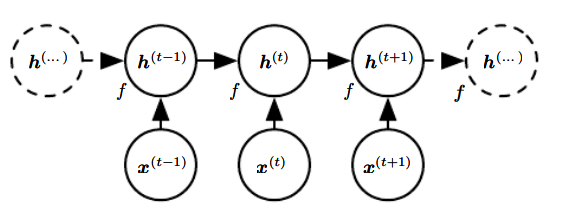
\includegraphics[]{images/recurrent-graph.png}
\end{center}
The state transition function can be represented using the time shift operator $q^{-1}$:
\[q^{-1}h^{(t)} = h^{(t-1)}\]
\begin{center}
    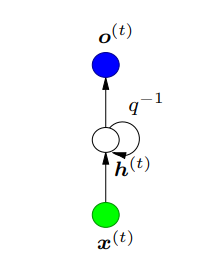
\includegraphics[]{images/time-shift-op.png}
\end{center}
The unfolding process thus introduces two major advantages:
\begin{enumerate}
    \item Regardless of the sequence length, the learned model always has the same input size, because it is specified in terms of transition from one state to another state, rather than specified in terms of a variable-length history of states.

    \item It is possible to use the same transition function $f$ with the same parameters at every time step.
\end{enumerate}
These two factors make it possible to learn a single model that operates on all time steps and all sequence lengths. Learning a single, shared model allows generalization to sequence lengths that did not appear in the training set, and allows the model to be estimated with far fewer training examples than would be required without parameter sharing.\newline\newline
Given a sequence $s \in X^{*}$ and a recursive transduction $T$, the \textit{encoding network} associated to $s$ and $T$ is formed by unrolling (time unfolding) the recursive network of $T$ through the input sequence $s$.
\begin{center}
    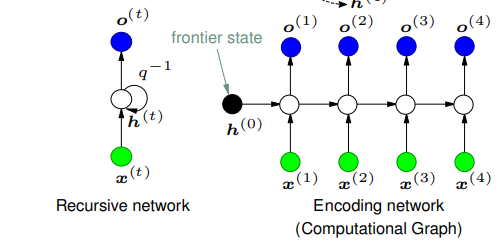
\includegraphics[]{images/encoding-network.png}
    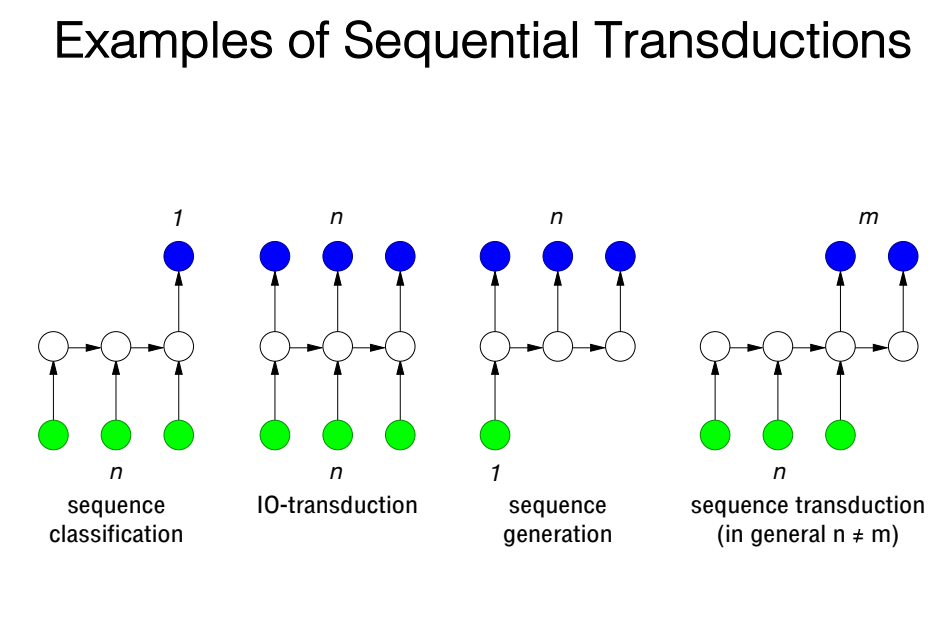
\includegraphics[scale=0.7]{images/sequential--transduction.png}
\end{center}
$T$ is \textbf{stationary} if $f(\cdot)$ and $g(\cdot)$ do not depend on $t$\newline\newline
There are different ways in which we can implement $f(\cdot)$ and $g(\cdot)$. There are two general families of models:
\begin{itemize}
    \item Linear:
    \begin{itemize}
        \item Kalman Filter
        \item Hidden Markov Models
        \item Linear Dynamical Systems
        \item ...
    \end{itemize}
    \item Nonlinear
    \begin{itemize}
        \item Recurrent Neural Networks
        \item ...
    \end{itemize}
\end{itemize}

\section{Shallow Recurrent Neural Networks}
Armed with the graph unrolling and parameter sharing ideas, we can design a wide variety of recurrent neural networks. In general we have:
\[\begin{split}
    \textbf{h}^{(t)} & = f(\textbf{U}\textbf{x}^{(t)} + \textbf{W}\textbf{h}^{(t-1)} + \textbf{b})\\
    \textbf{o}^{(t)} & = g(\textbf{V}\textbf{h}^{(t)} + \textbf{c})
\end{split}\]
where $f()$ and $g()$ are non-linear functions (e.g. $tanh()$ and $softmax$), and $h^{(0)} = 0$ (or can be learned jointly with the other parameters). $\textbf{U}$ and $\textbf{W}$ are weight matrices which parametrize \textbf{input-to-hidden} connections and \textbf{hidden-to-hidden} recurrent connections respectively. \textbf{Hidden-to-output} connections are parametrized by the weight matrix $\textbf{V}$.\newline\newline
An example of RNN for IO-transduction with discrete outputs:
\[\begin{split}
    \textbf{h}^{(t)} & = tanh(\textbf{U}\textbf{x}^{(t)} + \textbf{W}\textbf{h}^{(t-1)} + \textbf{b})\\
    \textbf{o}^{(t)} & = \textbf{V}\textbf{h}^{(t)} + \textbf{c}\\
    \hat{\textbf{y}} & = softmax(\textbf{o}^{(t)})\\
    L & = \sum_t L^{(t)} = - \sum_t log\,p_{model}(\textbf{y}^{(t)} | \{\textbf{x}^{1}, ..., \textbf{x}^{(t)}\})
\end{split}\]
where:
\begin{itemize}
    \item $o^{(t)}$ is the unnormalized log probabilities a time $t$
    \item $\textbf{y}^{(t)}$ is the target vector a time $t$
    \item $p_{model}(\textbf{y}^{(t)} | \{\textbf{x}^{1}, ..., \textbf{x}^{(t)}\}$ is given by reading the entry for $\textbf{y}^{(t)}$ from the model’s output vector $\hat{\textbf{y}}^{(t)}$, that is, the loss $L$ \textbf{internally computes} $\hat{\textbf{y}}$.
    \item $L$ is the loss function
\end{itemize}
The corresponding computation graph is the following
\begin{center}
    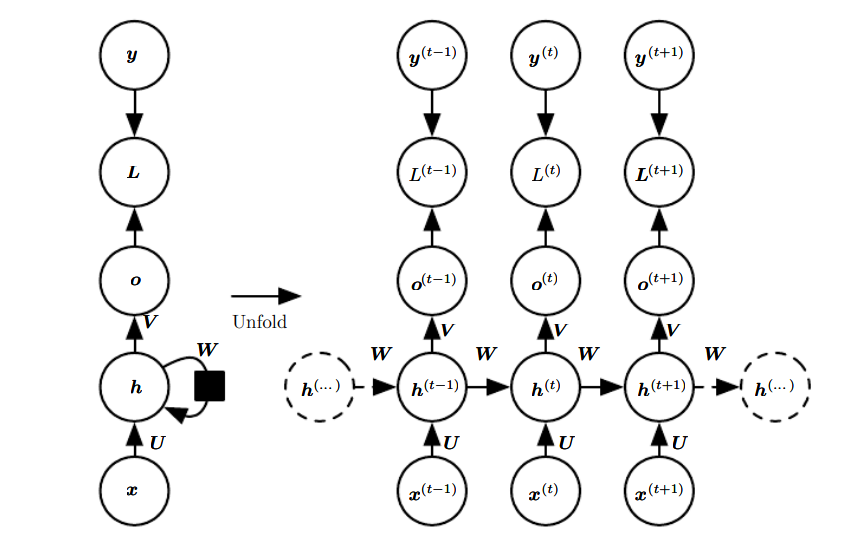
\includegraphics[scale=0.8]{images/rnn-computational-graph.png}
\end{center}
Some examples of important design patterns for recurrent neural networks
include the following:
\begin{itemize}
    \item Recurrent networks that produce an output at each time step and have recurrent connections between hidden units (IO-transduction).

    \item Recurrent networks that produce an output at each time step and have recurrent connections only from the output at one time step to the hidden units at the next time step

    \item Recurrent networks with recurrent connections between hidden units, that read an entire sequence and then produce a single output (e.g. for classification).
\end{itemize}
There are a lot of possible additional architectural features, such as short-cut connections, higher-order states, feedback from output, teacher forcing, bidirectional RNN, etc\footnote{See slides for further information}. All these architectural features (and others...) are orthogonal, i.e. they can be combined together.


\subsection{Teacher Forcing}
The network with recurrent connections only from the output at one time step to the hidden units at the next time step is strictly less powerful because it lacks hidden-to-hidden recurrent connections. Therefore, it requires that the output units capture all of the information about the past that the network will use to predict the future. Because the output units are explicitly trained to match the training set targets, they are unlikely to capture the necessary information about the past history of the input.\newline\newline
For this reason, models that have recurrent connections from their outputs leading back into the model may be trained with \textbf{teacher forcing}. Teacher forcing is a procedure in which during training the model receives the ground truth output $\textbf{y}^{(t)}$ as input at time $t + 1$. When the model is deployed, the true output is generally not known. In this case, we approximate the correct output $\textbf{y}^{(t)}$ with the model’s output $\textbf{o}^{(t)}$, and feed the output back into the model.
\[\begin{split}
    \textbf{h}^{(t)} & = tanh(\textbf{U}\textbf{x}^{(t)} + \textbf{W}\textbf{y}^{(t-1)} + \textbf{b})\\
    \textbf{o}^{(t)} & = \textbf{V}\textbf{h}^{(t)} + \textbf{c}\\
    \hat{\textbf{y}} & = softmax(\textbf{o}^{(t)})\\
    L & = - \sum_t log\,p_{model}(\textbf{y}^{(t)} | \textbf{y}^{(1)}, ..., \textbf{y}^{(t-1)}, \textbf{x}^{(1)}, ..., \textbf{x}^{(t)})
\end{split}\]
\begin{center}
    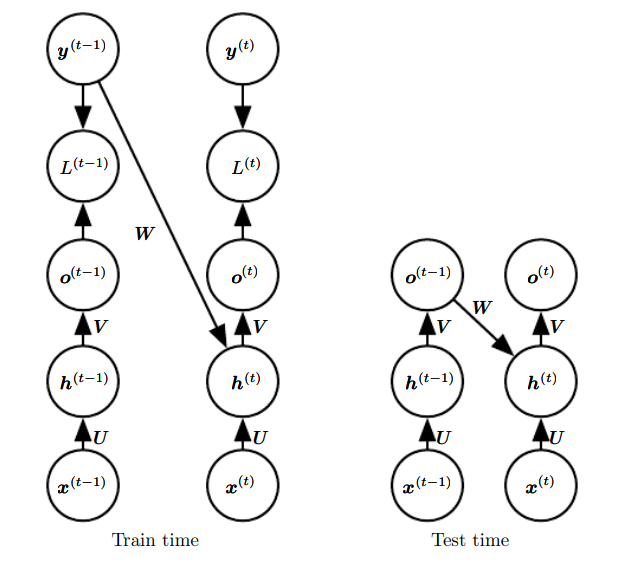
\includegraphics[]{images/teacher-forcing.png}
\end{center}
The advantage of eliminating hidden-to-hidden recurrence is that, for any loss function based on comparing the prediction at time $t$ to the training target at time $t$, all the time steps are decoupled. Training can thus be parallelized, with the gradient for each step $t$ computed in isolation.

\subsection{Bidirectional RNNs}
in many applications we want to output a prediction of $\textbf{y}^{(t)}$ which may depend on the whole input sequence. For example, if there
are two interpretations of the current word that are both plausible, we may have to look far into the future (and the past) to disambiguate them. Bidirectional recurrent neural networks (or bidirectional RNNs) were invented to address that need.\newline\newline
As the name suggests, bidirectional RNNs combine an RNN that moves forward
through time, beginning from the start of the sequence, with another RNN that moves backward through time, beginning from the end of the sequence.
\begin{center}
    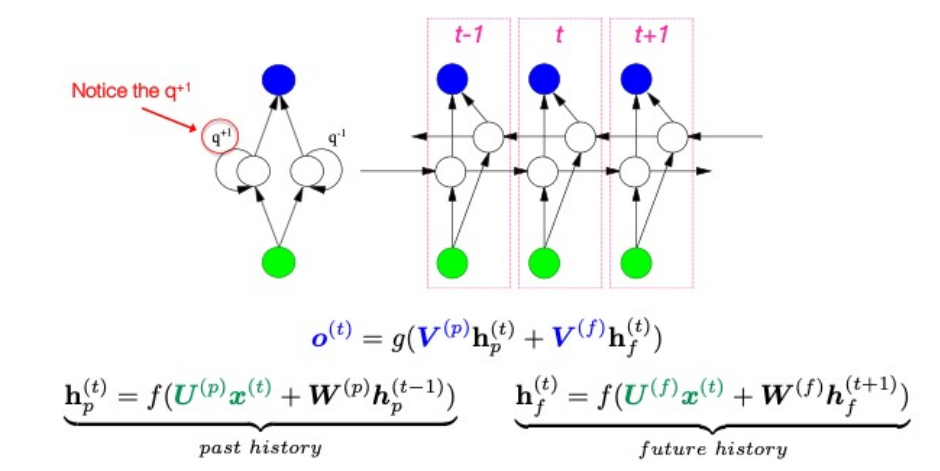
\includegraphics[scale=0.9]{images/bidirectional-rnn.png}
\end{center}

\subsection{1 to \textit{n} transduction}
Previously, we have discussed RNNs that take a sequence of vectors $\textbf{x}^{(t)}$ for $t = 1, ..., \tau$ as input. Another option is to take only a single vector $\textbf{x}$ as input. When $\textbf{x}$ is a fixed-size vector, we can simply make it an extra input of the RNN
that generates the $\textbf{y}$ sequence.  The interaction between the input $\textbf{x}$ and each hidden unit vector $\textbf{h}^{(t)}$ is parametrized by a newly introduced weight matrix $\textbf{R}$.
\begin{center}
    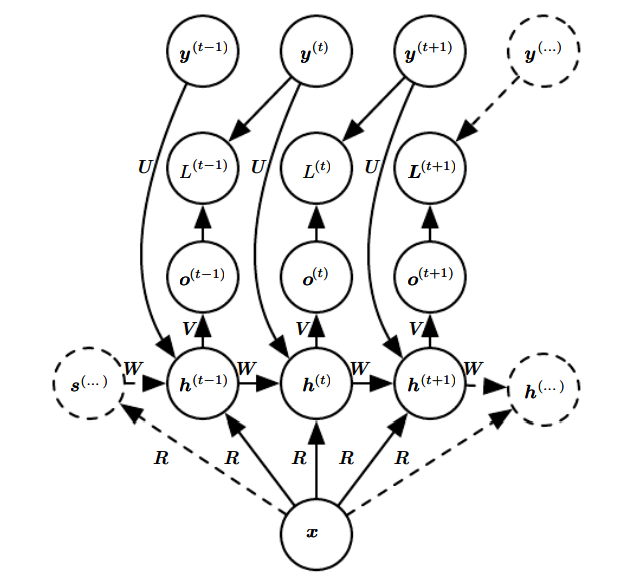
\includegraphics[scale=0.8]{images/1-to-n transduction.png}
\end{center}
Each element $\textbf{y}^{(t)}$ of the observed output sequence serves both as input (for the current hidden unit at time $t$) and, during training, as target (for the previous output unit at time $t-1$).\newline\newline
This RNN is appropriate for tasks such as image captioning, where a single image is used as input to a model that then produces a sequence of words describing the image.

\subsection{Encoder-Decoder Sequence-to-Sequence Architectures}
Here we discuss how an RNN can be trained to map an input sequence to an output sequence which is not necessarily of the same length. This comes up in many applications, such as speech recognition, machine translation, etc.\newline\newline
An encoder-decoder RNN architecture is is composed of an encoder RNN that reads the input sequence and a decoder RNN that generates the output sequence. The final hidden state of the encoder RNN is used to compute a generally fixed-size context variable $C$ which represents a semantic summary of the input sequence and is given as input to the decoder RNN.
\begin{center}
    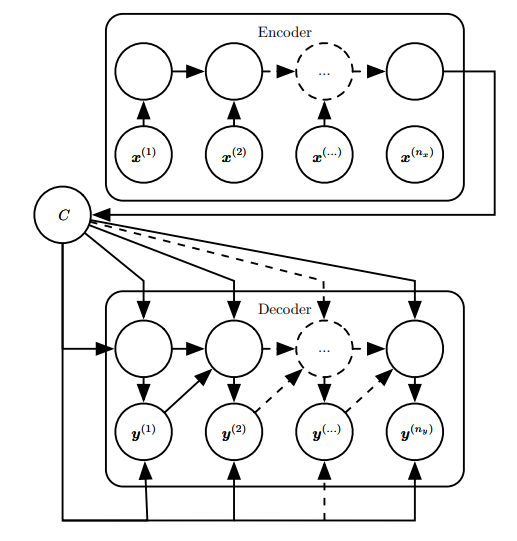
\includegraphics[]{images/encoder-decoder rnn.png}
\end{center}
If the context $C$ is a vector, then the decoder RNN is simply a vector-to-sequence RNN.


\chapter{Lec 16 - Graph Neural Networks}

\section{Introduction}
Traditional ML approaches have been developed assuming data to be encoded into feature vectors; however, many important real-world applications generate data that are naturally represented by more complex structures, such as graphs. Graphs are particularly suited to
represent the relations (arcs) between the components (nodes) constituting an entity. For instance, in social network data, single data “points” (i.e., users) are closely inter-related.\newline\newline
A graph $G = (V, E)$ can be represented using the so called \textbf{adjacency matrix}. A $n \times n$ matrix $A$ such that $A[i,j] = 1$ if $edge(i,j) \in E$, 0 otherwise.\newline\newline
    \textbf{Example:}\newline\newline
    \begin{center}
        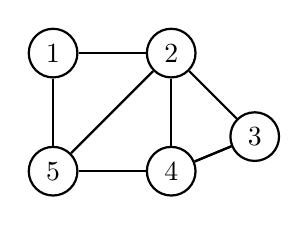
\begin{tikzpicture}[node distance={15mm}, thick, main/.style = {draw, circle}] 
            \node[main] (1) {$1$}; 
            \node[main] (2) [right of=1] {$2$}; 
            \node[main] (3) [below right of=2] {$3$}; 
            \node[main] (4) [below of=2] {$4$}; 
            \node[main] (5) [below of=1] {$5$}; 
            \draw (1) -- (2); 
            \draw (1) -- (5); 
            \draw (2) -- (5);
            \draw (2) -- (4);
            \draw (5) -- (4);
            \draw (3) -- (4); 
            \draw (5) -- (4);
            \draw (4) -- (3);
            \draw (2) -- (3);
        \end{tikzpicture}
    \end{center}
    The Adjacency matrix of the graph above is the following:
    \[\begin{bmatrix}
        0 & 1 & 0 & 0 & 1 \\
        1 & 0 & 1 & 1 & 1 \\
        0 & 1 & 0 & 1 & 0 \\
        0 & 1 & 1 & 0 & 1 \\
        1 & 1 & 0 & 1 & 0
    \end{bmatrix}\]
In undirected graphs this matrix is \textbf{symmetric}, while in directed graphs it is \textbf{asymmetric}. In case of a weighted graph, each cell of the matrix has either the value of the edge weight $w$ or $-$. Each node and edge is represented by a feature vector:
\begin{center}
    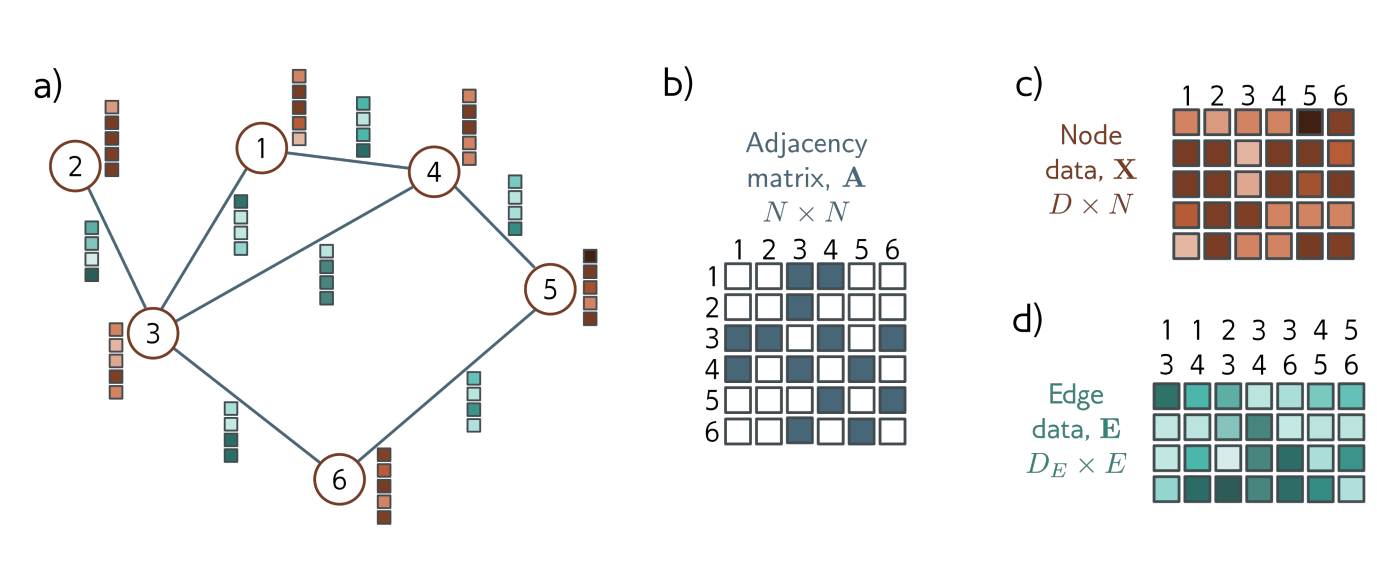
\includegraphics[scale=0.5]{images/graphs.png}
\end{center}
The position $(m,n)$, of the adjacency matrix contains the number of walks of length one from node $m$ to node $n$. Position $(m,n)$ of the \textbf{squared} adjacency matrix $A^2$ contains the number of walks of length two from node $m$ to node $n$.\newline\newline
The main problem settings that can arise when dealing with structured data are the following:
\begin{itemize}
    \item Predictions over \textbf{nodes} in a network: In this setting, the dataset is composed of a single (possibly disconnected) large graph. Each example is a node in the graph, and the learning tasks are defined as predictions over the nodes. Given an unseen node $u$, the task is to predict the correct target $y_u$. An example in this setting is the prediction of properties of a social network user based on his or her connections.

    \item Predictions over \textbf{graphs}: In this case, each example is composed of a whole graph, and the learning tasks are predictions of properties of the whole graphs. An example is the prediction of toxicity in humans of chemical compounds represented by their molecular graph.

    \item Link-prediction tasks: the model predicts whether or not there should be an edge between nodes. 
\end{itemize}

\section{Learning on graphs is difficult}
Let $\textbf{X}$ be the matrix in which the feature vectors of each node are stored. We can observe that node indexing in graphs is arbitrary. This means that, differently from images, permuting the node indices results in a permutation of the columns of $\textbf{X}$ and a permutation of both the rows and columns of $A$. However, the underlying graph is unchanged. This property is called Permutation Invariance. More formally, given a permutation matrix $\textbf{P}$, we get a different representation of the same graph:
\[\begin{split}
    \textbf{X}' & = \textbf{XP}\\
    \textbf{A}' & = \textbf{P}^T \textbf{AP}
\end{split}
\]
This property can give the intuition about why learning on graphs is difficult. In fact, determining if two graphs are equal (graphs isomorphism) is a problem for which are not known polynomial-time algorithms. Furthermore, sub-graph isomorphism, which is the problem of determining if a graph is a sub-graph of another graph, is NP-Complete. These problems affect machine learning because a model should be able to predict the same output for isomorphic graphs (which can be represented in different ways). Furthermore, the model we design should capture the similarity between two graphs (sub-graph isomorphism).\newline\newline
In general, the main problems we face when learning on graphs are the following:
\begin{enumerate}
    \item Same graph can be represented in different ways;
    \item How to recognize that a given graph $G_2$ is a sub-graph of $G_1$
    \item How to represent graphs of different sizes (i.e., different number of nodes) into fixed-size vectors without loosing expressiveness ?

    \item How to avoid explosion in the number of parameters with the size of the graphs?
    
\end{enumerate}
Problem 3 is commonly faced by using recursive models that exploit a
causal state space [Sperduti \& Starita., TNN 1997], while Problem 4  is commonly faced by exploiting shared parameters.\newline\newline
Regarding Problems 1 and 2, a sound and meaningful representation for graphs can be achieved by using a neural network with \textbf{convolution operator}, defined on graphs.

\section{Graph Neural Networks - General Idea}
A Graph Neural Network (GNN) receives in input a graph (adj. matrix and node representations. for simplicity) and passes it through a series of $k$ layers. Each layer computes a hidden representation for each node, with the last layer computing the final nodes' embeddings $\textbf{H}_k$. Similarly to CNNs, each node representation includes information about the node and its context within the graph.
\begin{itemize}
    \item For \textbf{node-level tasks}, the output is computed from $\textbf{H}_k$;

    \item For \textbf{graph-level tasks}, the nodes' embeddings are combined (e.g., by averaging), and the resulting vector is mapped via a linear transformation or neural network to a fixed-size vector from which the classification/regression task is performed.

    \item For \textbf{link-prediction tasks}, the embeddings of the two endpoint nodes must be mapped to a single number representing the probability that the edge is present (e.g. dot product of the nodes' embeddings and pass the result through a sigmoid function to create a probability).
 
\end{itemize}
\begin{center}
    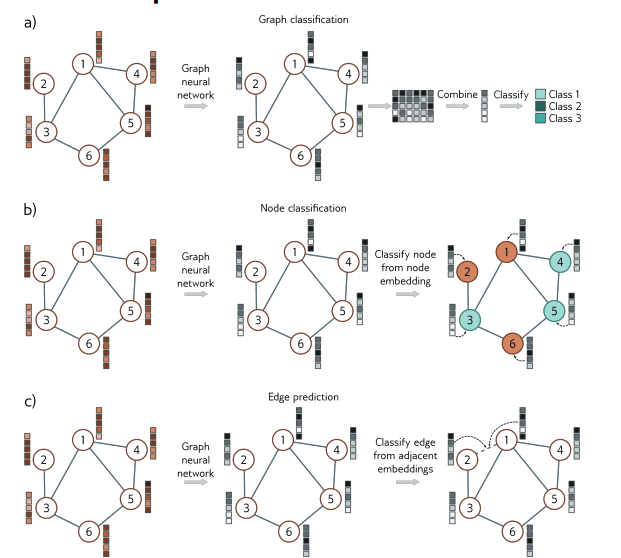
\includegraphics[]{images/gnn.png}
\end{center}

\section{Graph Convolution}
The general idea of graph convolution starts from a parallel between graphs and images. GNNs implement convolution in a similar way how CNNs do, that is, learning the features by inspecting neighboring nodes. GNNs generalize the definition of convolution for non-regular structured data.

\subsection{NN4G by Micheli}
\textbf{NN4G} is an architecture based on a graph convolution that is defined as:
\begin{center}
    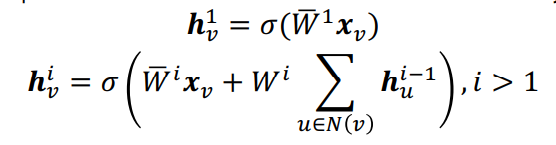
\includegraphics[scale=0.6]{images/nn4g.png}
\end{center}
where: 
\begin{itemize}
    \item $\sigma$ is a nonlinear activation function applied element-wise.
    \item $N(v)$ represent the neighborhood of node $v$.
    \item $\textbf{W}^i$ is a weights' matrix;
    \item $\textbf{x}_u$ is the feature vector of node $u$.
\end{itemize}
Actually, this is a simplified notation, since the original one uses skip connections (see GNN book chapter).
\begin{center}
    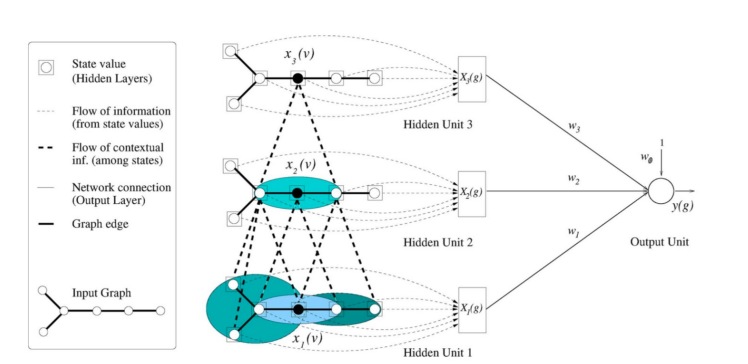
\includegraphics[]{images/nn4g-2.png}
\end{center}
Note that:
\begin{itemize}
    \item The first layer ($i = 1$), which has no previous layers, computes the nodes' representations only on the basis of each vertex feature vector.

    \item Each convolution performed on the $i$-th hidden units, with $i > 1$, takes as input the neighbors' representations of the previous layer. Basically, it merges the representations of each node with those of its neighbors:

    \item $X_1(g), X_2(g), X_3(g)$ are scalar values computed by aggregating the representations $\textbf{x}_i(g)$ for each unit $i$.
    In particular they are defined as:
    \[X_i(g) = \frac{1}{k}\sum_{v \in Vert(g)}x_i(v)\]
    if $k = 1$, this corresponds to a sum. Basically, we compute a representation per-graph per-layer. Then, this 3 representations are parametrized by the weights $w_1, w_2, w_3$ and used to compute the output for the whole graph (graph-level task).
\end{itemize}
The convolutional operation presented above can be defined in a compact way using matrix multiplications:
\begin{center}
    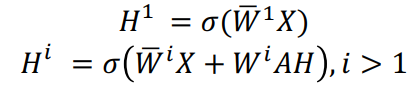
\includegraphics[scale=0.6]{images/matrix-gcn.png}
\end{center}
where $\textbf{A}$ is the adjacency matrix. Exploiting matrix multiplications makes the computation really fast. Furthermore, note that, as for images, the receptive field of the layers increases as we stack more layers.\newline\newline
Note also that, since with the convolution operator we are merging neighboring nodes' representations, isomorphic graphs in which the order of the nodes is changed will have the same nodes' representations.

\subsection{Graph Fourier Transform}
The operation described above is graph convolution, but how it is derived? Defining the formal convolution operator on graph is difficult.\newline\newline
Let $x: V \rightarrow \mathbb{R}$ be a signal on the nodes $V$ of the graph $G$, i.e., a function that associates a real value with each node of $V$. We can represent every signal as a vector $\textbf{x} \in \mathbb{R}^n$, which from now on we will refer to as signal. In order to set up a convolutional network on $G$, we need the notion of convolution between a signal $\textbf{x}$ and a filter signal $\textbf{f}$.\newline\newline
The key idea is to use a Fourier transform. In the frequency domain, thanks to the \textbf{Convolution Theorem}, the (undefined) convolution of two signals becomes the (well-defined) component-wise product of their transforms. So, if we knew how to compute the Fourier transform of a function defined on a graph, we could define the convolution operator.\newline\newline
The Convolution Theorem states that convolution in one domain (time, space) corresponds to pointwise multiplication in frequency domain.\newline\newline
The \textbf{graph Fourier transform} is defined starting from the (normalized) Laplacian matrix of the graph, which is defined as:
\[L = I_n - D^{-\frac{1}{2}} A D^{-\frac{1}{2}}\]
where:
\begin{itemize}
    \item $I_n$ is the identity matrix;
    \item $A$ is the adjacency matrix;
    \item $D$ is the degree matrix, that is, the \textbf{diagonal} matrix containing the number of edges attached to each vertex;
\end{itemize}
Then, we can compute the eigendecomposition of $L$ (which is always possible):
\[L = U \Lambda U^T\]
where $\Lambda = diag([\lambda_0, ..., \lambda_{n-1}])$ and $U$ is the Fourier basis of the graph.\newline\newline
Finally, Given a spatial signal $\textbf{x}$:
\begin{itemize}
    \item $\hat{\textbf{x}} = U^T\textbf{x}$ is its graph Fourier Transform

    \item $\textbf{x} = U \hat{\textbf{x}}$ is the inverse Fourier transform
\end{itemize}
Therefore, convolution between a parametric filter and a signal can be defined as:
\[y = \textbf{f}_\theta *_G \textbf{x} = U\left( (U^T\textbf{f}_\theta) \odot (U^T \textbf{x})\right)\]
It can be proved that this operator corresponds to the one used for NN4G presented previously (see slides for more details).

\section{Aggregation Layer for graph classification}
With Graph Convolution we have a representation for each graph node. How can we map node representations to a graph-level representation? There are some simple solutions, like the sum or the average of nodes' representations as we saw previously, or we can rely on more complex alternatives: Universal readout.


\section{Graph Recurrent Neural Networks}
Scarselli et al. proposed a network architecture where, instead of stacking multiple layers, a single recurrent layer is adopted:
\[\textbf{h}_v^{t+1} = \sum_{u \in N(v)}f(\textbf{h}_u^t, \textbf{x}_v, \textbf{x}_u)\]
where $f$ is a function (e.g. neural network) with shared parameters across all the nodes and all the time steps. The recurrent system is defined as a contraction mapping, and thus it is guaranteed to converge to a fixed point $\textbf{h*}$.

\subsection{Gated Graph Neural Networks}
The idea is to remove the constraint for the recurrent system to be a contraction mapping, and implement this idea by adopting recurrent
neural networks to define the recurrence. Specifically, the gated recurrent unit (GRU) is adopted. The recurrent convolution operator is defined as follows:
\begin{center}
    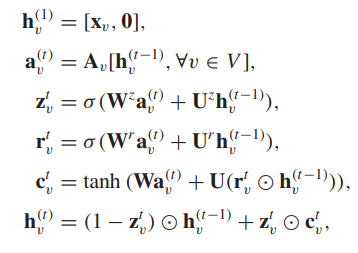
\includegraphics[scale=0.8]{images/gated-gnn.png}
\end{center}
where $\textbf{A}_v$ is row $v$ of the adjacency matrix $\textbf{A}$.


\chapter{Back-Propagation Through Time}

\section{BPTT}
\begin{figure}
    \centering
    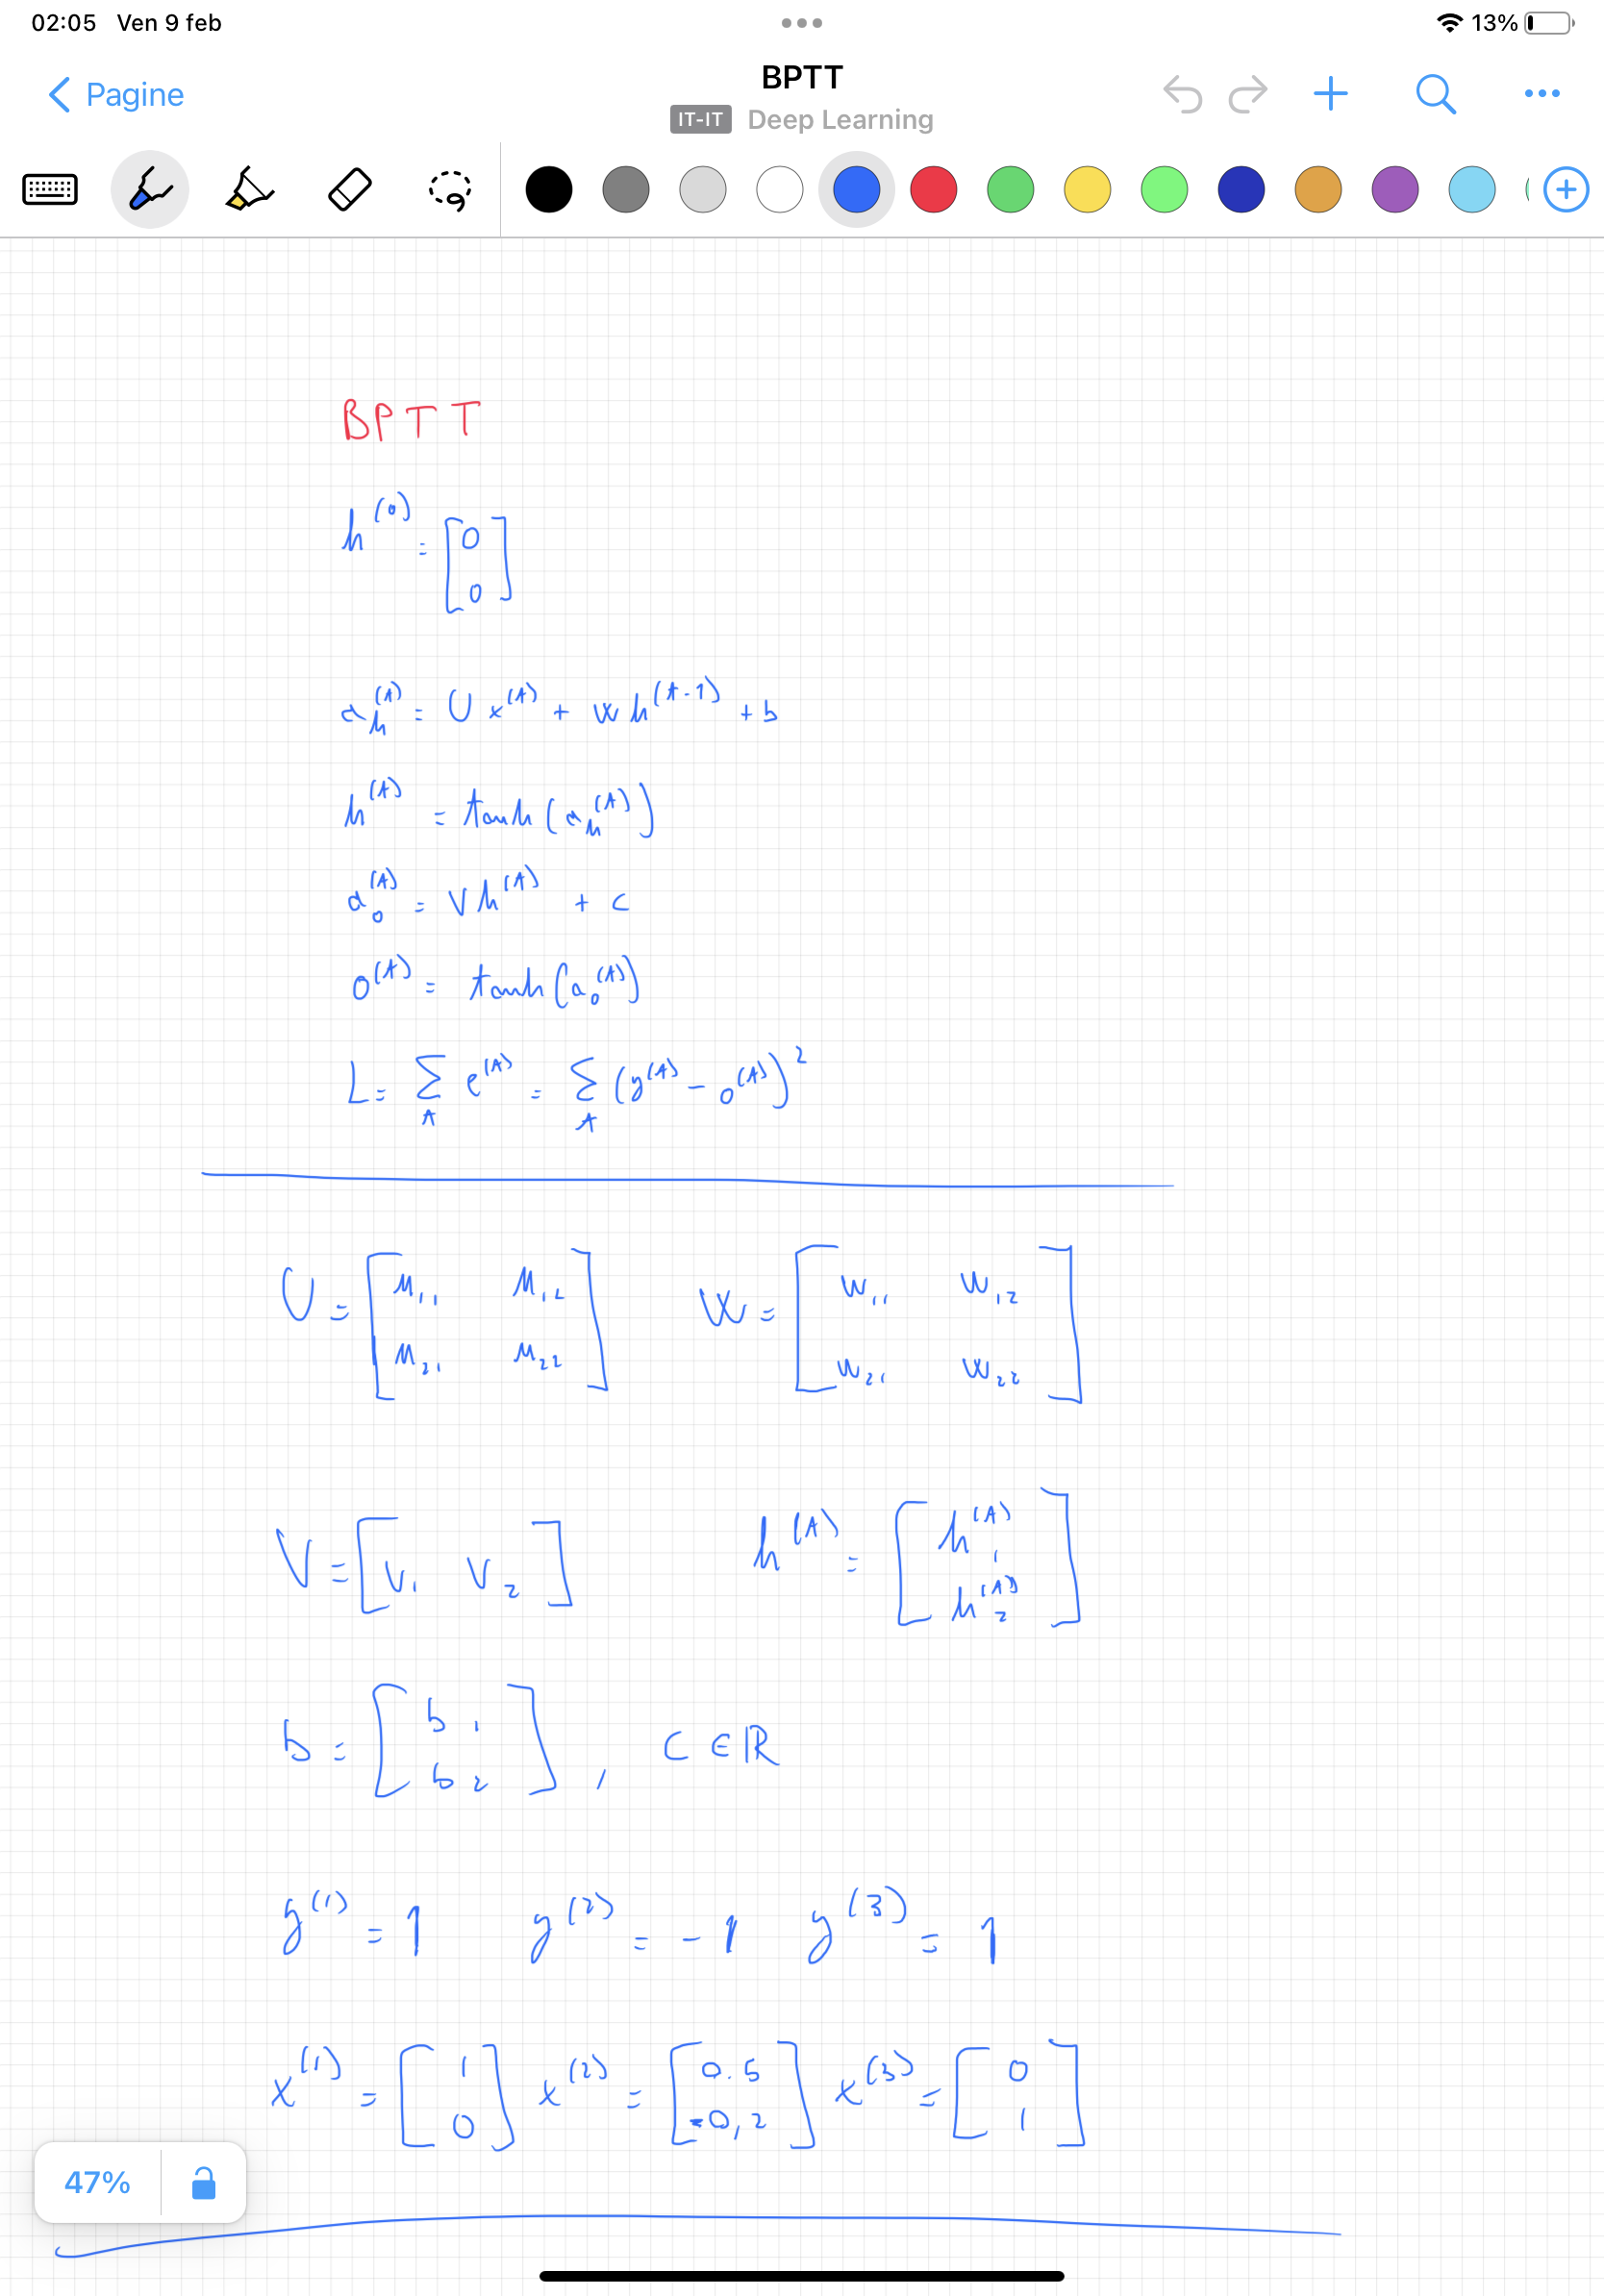
\includegraphics[scale=0.2]{images/bptt_1.PNG}
    \label{fig:enter-label}
\end{figure}
\begin{figure}
    \centering
    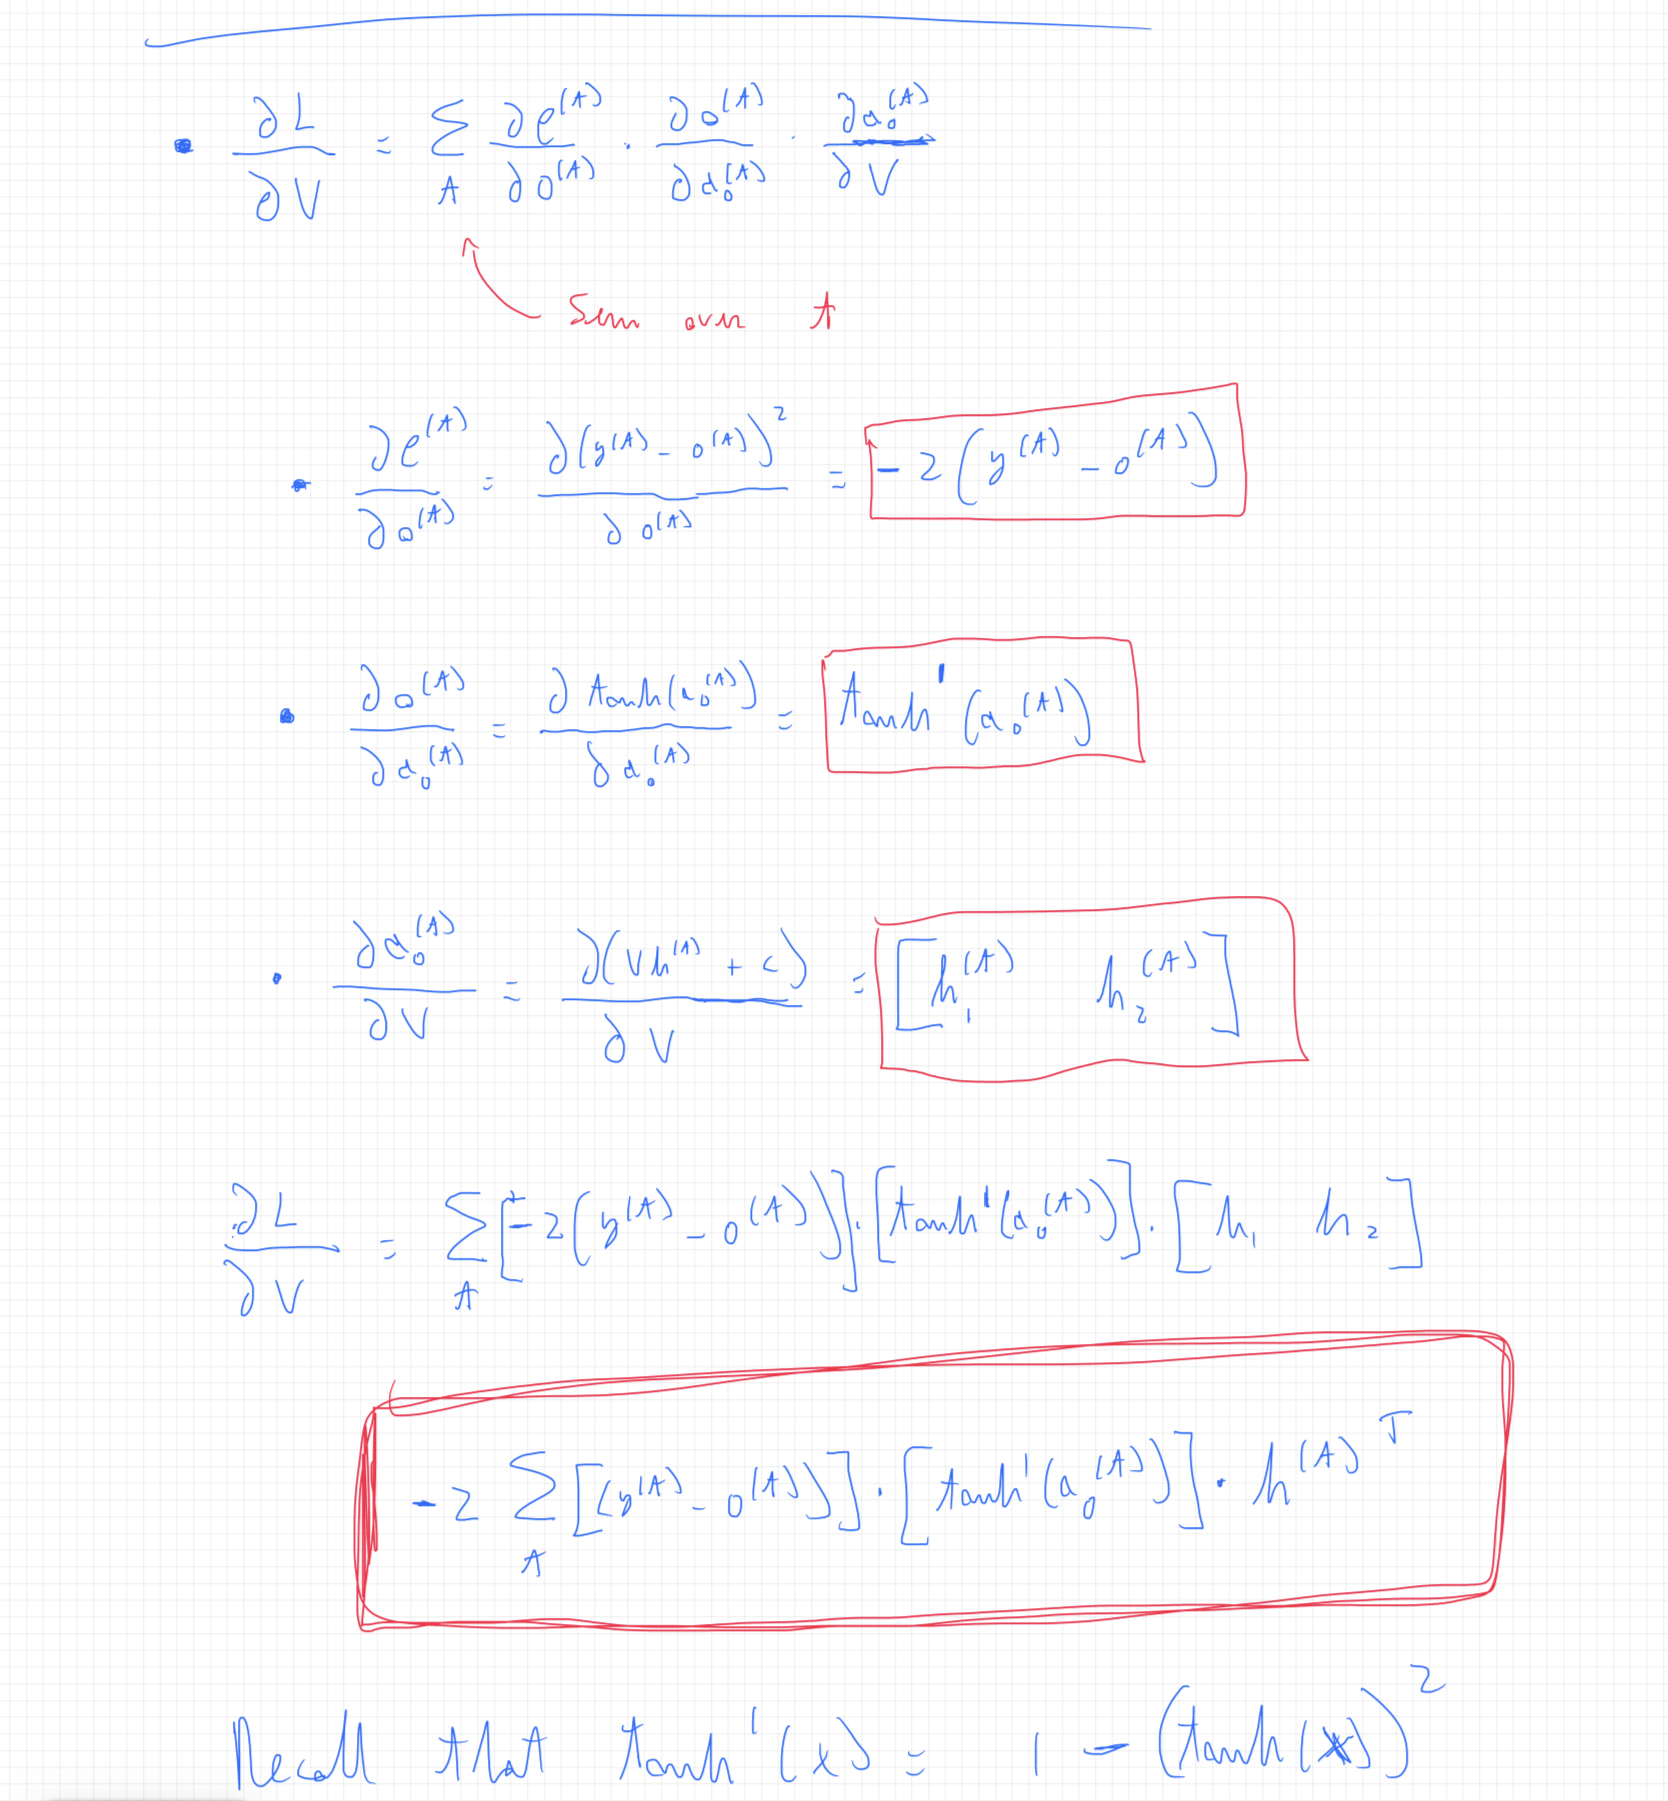
\includegraphics[scale=0.2]{images/bptt_2.jpg}
    \label{fig:enter-label}
\end{figure}
\begin{figure}
    \centering
    \includegraphics[scale=0.3]{images/bptt_3.jpg}
    \label{fig:enter-label}
\end{figure}
\begin{figure}
    \centering
    \includegraphics[scale=0.3]{images/bptt4.jpg}
    \label{fig:enter-label}
\end{figure}
\chapter{Lec 18 - Long-Term Dependencies}

\section{Learning Long-Term Dependencies}
The basic problem of learning long-term dependencies is that gradients propagated over many stages tend to either vanish (most of the time) or explode\footnote{a problem when large error gradients accumulate and result in very large updates to neural network model weights during training} (rarely, but with much damage to the optimization).\newline\newline
A long-term dependency is when the desired output at time $t$ depends on the input at time $t - \tau$, with $t > \tau >> 1$ (e.g. $\textbf{x}^{(t - 100)} \rightarrow \textbf{y}^{(t)}$).\newline\newline
This means that, for the Recurrent Neural Network to output the correct
desired $\textbf{y}^{(t)}$, it has to recognize its dependency on $\textbf{x}^{(t - \tau)}$, and use $\textbf{x}^{(t - \tau)}$ in the generation of $\textbf{y}^{(t)}$.
\newline\newline
Here are some approaches to try to reduce the vanishing/exploding gradients
problem:
\begin{itemize}
    \item Architectural
    \begin{itemize}
        \item Long Short-Term Memory or Gated Recurrent units
        \item Reservoir Computing: Echo State Networks and Liquid State Machines
    \end{itemize}
    \item Algorithmic
    \begin{itemize}
        \item Clipping gradients (avoids exploding gradients)
        \item Hessian Free Optimization
        \item Smart Initialization: pre-training techniques
    \end{itemize}
\end{itemize}

\section{Long Short-Term Memory}
Long Short Term Memory networks - usually just called “LSTMs” - are a special kind of RNN, capable of learning long-term dependencies.\newline\newline
They are based on the idea of creating paths through time that have derivatives that neither vanish nor explode.\newline\newline
The mechanism allows the networks to “remember” relevant information for a long period of time and to "forget" them when they are no more relevant.
\newline\newline
The LSTM does have the ability to remove or add information to the cell state, carefully regulated by structures called gates. Gates are a way to optionally let information through. They are composed out of a sigmoid neural net layer and a pointwise multiplication operation. The sigmoid layer outputs numbers between zero and one, describing how much of each component should be let through. A value of zero means “let nothing through,” while a value of one means “let 
verything through!”
\newline\newline
An LSTM has three of these gates, to protect and control the cell state:
\begin{enumerate}
    \item Forget gate: The sigmoid layer called the “forget gate layer ”\textit{decides} what information we’re going to throw away from the cell state. It looks at $h^{(t-1)}$ and $x^{(t)}$, and outputs a number between 0 and 1 for each number in the cell state $C^{(t-1)}$ . A 1 represents “completely keep this” while a 0 represents “completely get rid of this.” Let $f_t$ be its output. The forget gate multiplies the old state by $f_t$, forgetting the things it decided to forget.
    \begin{center}
        \includegraphics[]{images/forget-gate.png}
    \end{center}

    \item Input gate: It decides what new information are going to be stored in the cell state. This has two parts. First, a sigmoid layer called the “input gate layer” decides which values are going to be updated. Let $i^t$ be its output. Next, a tanh layer creates a vector of new candidate values, $\Tilde{C^t}$, that could be added to the state. The input gate computes $i^t * \Tilde{C^t}$. The output of this gate is added to the output of the forget gate to determine the new cell state.
    \begin{center}
        \includegraphics[]{images/Input-gate.png}
        \includegraphics[scale=0.9]{images/new cell-state.png}
    \end{center}
    
    \item Output gate: It deterines what parts of the cell state are going to be outputted. It puts the cell state through tanh (to push the values to be between -1 and 1). The result is multiplied by the output of a sigmoid layer so that it only outputs the parts it decided to.
    \begin{center}
        \includegraphics[]{images/output-gate.png}
    \end{center}
\end{enumerate}
There are a lot of variations of the LSTM architecture. One popular variant is adding “peephole connections.” This means that we let the gate layers look at the cell state. Other variations are:
\begin{itemize}
    \item No Input Gate (NIG)
    \item No Forget Gate (NFG)
    \item No Output Gate (NOG)
    \item No Input Activation Function (NIAF)
    \item No Output Activation Function (NOAF)
\end{itemize}
However, vanilla LSTM performs reasonably well in general and variations do not significantly improve the performance. Furthermore, the forget gate is crucial for LSTM performance.

\section{Simplifying LSTM: Gated Recurrent Units}
The main difference between GRU and LSTM is that GRU uses a single gating unit that simultaneously controls the forgetting factor and the decision to update the state unit.
\begin{center}
    \includegraphics[]{images/GRU.png}
\end{center}
The update gate $\textbf{z}$ selects whether the hidden state need to be updated with a new hidden state $\Tilde{\textbf{h}}$. The reset gate $\textbf{r}$ decides whether the previous hidden state is ignored.\newline\newline
The values for $\textbf{z}$ and $\textbf{r}$ are defined as usual using the sigmoidal layers as in LSTM.\newline\newline
Basically, the idea is that if the $\textbf{z}$ vector has a value equal to 0 in position $i$, when we compute the element-wise multiplication between $\textbf{z}$ and $\textbf{h}^{(t-1)}$ the $i$-th value in $\textbf{h}^{(t-1)}$ will be cancelled. On the other hand, the $i$-th element in $(1 - \textbf{z})$ is 1. Therefore, the $i$-th element of $\textbf{h}^{(t-1)}$ will be updated with the $i$-th element of $\Tilde{\textbf{h}}$.

\section{Reservoir Computing}
Reservoir Computing is an umbrella term used to identify a general framework of computation derived from Recurrent Neural Networks (RNN). This technique can be implemented with \textbf{Echo State Networks} and \textbf{Liquid State Machines}. The idea is to fix the input-to-hidden and hidden-to-hidden connections at random values and only learn the output units connections. The intuition was born from the fact that in training RNNs most of the times the weights showing most change were the ones in the last layer.\newline\newline
The first part of the system, called Reservoir, is an RNN with fixed weights that acts as ”black-box” model of a complex system; The second one is known as Readout, a classifier layer of some kind, usually a simple linear one, connected by a set of weights to the Reservoir.\newline\newline
One way to think about these reservoir computing recurrent networks is that they are similar to kernel machines: they map an arbitrary length sequence (the history of inputs up to time $t$) into a fixed-length vector (the recurrent state $\textbf{h}^{(t)}$), on which a linear predictor (typically a linear regression) can be applied to solve
the problem of interest.\newline\newline
How do we set the input and recurrent weights so that a rich set of histories can be represented in the recurrent neural network state? in order to produce a “rich” set of dynamics, the reservoir should
\begin{itemize}
    \item be big (hundreds to thousands units).
    
    \item be sparsely (hidden weight matrix W up to 20\% possibile connections) and randomly (uniform distribution symmetric around zero) connected.

    \item satisfy the echo state property, i.e., the ability to forget information from the far past (or the effect of $\textbf{x}^{(t)}$ and $\textbf{h}^{(t)}$ on the future state should vanish gradually as time passes). This means that the spectral radius $\rho(\textbf{W}) < 1$, i.e, $\textbf{W}$ is contractive. 

    \item On the contrary, the input ($U$) and optional output feedback weight matrices are dense (still random with uniform distribution).
    
\end{itemize}
\textbf{Echo State Networks} are composed of standard standard recurrent neurons plus leaky integrators, while \textbf{Liquid State Machines} implements spiking integrate-and-fire neurons and dynamic synaptic connection models. A leaky integrator is defined as follows:
\[\textbf{h}^{(t)} = (1 - a)\textbf{h}^{(t-1)} + \sigma(\textbf{U} \textbf{x}^{(t)} + \textbf{W}\textbf{h}^{(t-1)})\]
Basically, it adds a portion of the previous state representation (according to $a$) to the new state representation.\newline\newline 
If the network is too contractive, it will forget too quickly information from the past. In order to overcome this problem we can use the \textbf{intrinsic plasticity} approach. The main idea is to exploit the full range of output of the activation function of the hidden units. IP is a computationally efficient online learning rule to adjust threshold and gain of sigmoid reservoir neurons. It drives the neurons’ output activities to approximate exponential distributions. The exponential distribution maximizes the entropy of a non-negative random variable with a fixed mean, thus enabling the neurons to transmit maximal information\newline\newline
To evaluate  a RC network we use memory capacity, which tells us if the internal state of the network can reproduce input from the far past :
\[\sum_{k=0}^\infty r^2 (\textbf{x}^{(t - k)}, \textbf{o}_k^{(t)})\]
where $r^2 (\textbf{x}^{(t - k)}, \textbf{o}_k^{(t)})$ is the squared correlation coefficient between the input $\textbf{x}^{(t - k)}$ with delay $k$ and the corresponding output $\textbf{o}_k^{(t)}$ generated by the network at time $t$ for delay $k$.

\section{Deep Recurrent Networks}
The computation in most RNNs can be decomposed into three blocks of parameters
and associated transformations:
\begin{enumerate}
    \item  from the input to the hidden state,
    \item  from the previous hidden state to the next hidden state, and
    \item  from the hidden state to the output.
\end{enumerate}
With the RNN architecture, each of these three blocks is associated with a single weight matrix. In other words, when the network is unfolded, each of these corresponds to a shallow transformation. By a shallow transformation, we mean a transformation that would be represented by a single layer within a deep MLP. Typically this is a transformation represented by a learned affine transformation followed by a fixed nonlinearity.\newline\newline
Experimental evidence shows a significant advantage if the state of an RNN is decomposed into multiple layers.  We can think of the lower layers in the hierarchy as playing a role in transforming the raw input into a representation that is more appropriate at the higher levels of the hidden state.\newline\newline
However, in general, it is easier to optimize shallow architectures and adding depth may hurt learning by making optimization difficult.


\chapter{Lec 19-20 - Minimum cut}

\section{Classification of randomized algorithms}
\begin{enumerate}
    \item Randomized algorithms that never fail. They are called \textit{LAS VEGAS} algorithms (e.g. randomized quicksort).
    \[\forall i \in I, \, A_R(i) = s \,\, \text{s.t. } (i,s) \in \Pi\]
    where $\Pi \subseteq I \times S$ is a computational problem.\newline\newline
    Randomness comes into play in the analysis of the complexity. $\forall n, \,\,T(n)$\footnote{$T(n)$ is called complexity function} is a \textbf{random variable} of which we usually study its expectation $E[T(n)]$.\newline\newline
    If $P(T(n) > c \dot f(n)) \leq \frac{1}{n^k}$ for some constants $c$ and $k$, then we say that $T(n) = O(f(n))$ \textbf{with high probability}.

    \item Randomized algorithms that may fail. They are called \textit{MONTE CARLO} algorithms (e.g. verifying polynomial identity).
    \[\forall i \in I, \,\, \text{it's possible that } A_R(i) = s \,\, \text{s.t. } (i,s) \notin \Pi\]
    We study the probability $P((i,s) \notin \Pi)$ as a function of the input size $|i| = n$.\newline\newline
    For decision problems, these algorithms can be divided in two classes:
    \begin{itemize}
        \item \textbf{One-sided:} They may fail only on one answer.

        \item \textbf{Two-sided:} They may fail in both answer.
    \end{itemize}
\end{enumerate}

\section{Terminology}
\textbf{Definition:} Given a computational problem $\Pi \subseteq I \times S$, an algorithm $A_\Pi$ has complexity $T(n) = O(f(n))$ \textbf{with high probability} (w.h.p.) if $\exists$ constants $c, d > 0$ such that $\forall i \in I$ of size $n$ the following probability holds:
\[P(A_\Pi(i)\,\, \text{terminates in $> c\cdot f(n)$ steps}) \leq \frac{1}{n^d}\]
Then the probability of having a complexity of $O(f(n))$ is $> 1 - \frac{1}{n^d}$, that is, tends to 1 as $n$ tends to $\infty$.\newline\newline
\textbf{Definition:} Given a computational problem $\Pi \subseteq I \times S$, an algorithm $A_\Pi$ is correct w.h.p. if $\exists$ constant $d > 0$ such that $\forall i \in I, \,\, |i| = n$:
\[P((i, A_\Pi(i)) \notin \Pi) \leq \frac{1}{n^d}\]
\textbf{Markov's lemma:} Let $T$ be a non-negative, bounded ($\exists b \in \mathbb{N} \,\, \text{s.t. } P(T > b) = 0$), integer random variable. Then, $\forall t \,\, \text{such that } 0 \leq t \leq b$:
\[t \cdot P(T \geq t) \leq E[T] \leq t + (b - t)P(T \geq t)\]
\textbf{Application of Markov's lemma:}
Given a \textit{LAS VEGAS} algorithm $A_\Pi$, assume that:
\begin{enumerate}
    \item $T_{A_\Pi}(n) = O(f(n))$ with high probability, in particular, $P(T_{A_\Pi}(n) > c \cdot f(n)) \leq \frac{1}{n^d}$.

    \item $A_\Pi$ has a worst-case deterministic complexity $O(n^a), \,\, a \leq d \,\, \forall n$
\end{enumerate}
We can use Markov's lemma to prove the following property:
\[E[T_{A_\Pi}(n)] = O(f(n))\]
\textbf{Proof:} Just apply Markov's lemma:
\[E[T_{A_\Pi}(n)] \leq c \cdot f(n) + (n^a - c \cdot f(n)) \cdot \frac{1}{n^d} \leq c \cdot f(n) + \frac{n^a}{n^d} \leq c \cdot f(n) + 1\]
where:
\begin{itemize}
    \item $c \cdot f(n)$ is $t$
    \item $(n^a - c \cdot f(n))$ is $b - t$
    \item $\frac{1}{n^d}$ is $P(T \geq t)$
\end{itemize}


\section{Karger's algorithm for Minimum cut}
The minimum cut problem is finding a cut of minimum size, that is, the minimum number of edges whose removal disconnects the graph.\newline\newline
Karger's algorithm actually solves a more general problem: minimum cut on \textbf{multigraphs} (i.e. multiple edges between two vertices are allowed).\newline\newline
\textbf{Definition:} A \textbf{multiset} is a collection of objects with repetitions allowed.
\[S = \{\{\text{objects}\}\}\]
where $\forall \, \text{object }o \in S$, $m(o) \in \mathbb{N} \setminus \{0\}$ is called multiplicity, that is, how many copies of $o$ are in $S$.\newline\newline
\textbf{Definition:} We denote a multigraph as follows: $G = (V, E)$ where $V \subseteq \mathbb{N}$ and $E$ is a multiset of elements $(u,v)\,\, u \neq v$.\newline\newline
\textbf{Example:}\newline\newline
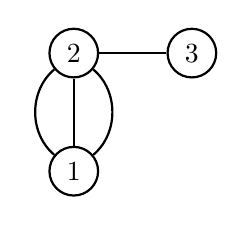
\begin{tikzpicture}[node distance={15mm}, thick, main/.style = {draw, circle}] 
            \node[main] (1) {$1$}; 
            \node[main] (2) [above of=1] {$2$}; 
            \node[main] (3) [right of=2] {$3$}; 

            \draw (1) edge[bend right = 50] (2); 
            \draw (1) -- (2); 
            \draw (1) edge[bend left = 50] (2);
            \draw (2) -- (3);
\end{tikzpicture}\newline\newline
A simple graph is also a multigraph.\newline\newline
\textbf{Definition:}Given a connected multigraph $G = (V, E)$. A cut $C \subseteq E$ is a multiset of edges such that $G' = (V, E \setminus C)$ is not connected.\newline\newline
\textbf{Karger's algorithm (simplified version):}
\begin{enumerate}
    \item Choose an edge at random;
    \item \textit{Contract} the two vertices of that edge;
    \item Repeat until only two vertices remain;
    \item Return the edges between them;
\end{enumerate}
\textbf{Definition:} Given a multigraph $G=(V,E)$ and an edge $e = (u, v)$, the \textbf{contraction} of $G$ with respect to $e$ is: $G_{/e} = (V', E')$ where:
\begin{itemize}
    \item $V' = V \setminus \{u, v\} \cup \{z_{u,v}\}$ where $z_{u,v} \notin V$.

    \item $E' = E \setminus \{\{ (x,y) : (x = u)\,\, \text{or}\,\, (x = v)\}\} \cup \{\{ (z_{u,v}, y) : (u, y) \in E \,\, \text{or} \,\, (v, y) \in E, \,\, y \neq u \,\, \text{and} \,\, y \neq v   \}\}$
\end{itemize}
It follows that:
\begin{itemize}
    \item $|V'| = |V| - 1$

    \item $|E'| = |E| - m(e) \leq |E| - 1$
\end{itemize}
Basically, it makes the two vertices to collapse in just one vertex connected with all the previous adjacent vertices. If as a result there are several edges between some pairs of (newly formed) vertices, retain them all.\newline\newline
\textbf{Example:}\newline\newline
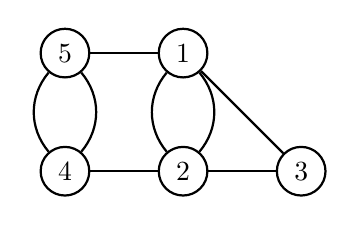
\begin{tikzpicture}[node distance={15mm}, thick, main/.style = {draw, circle}] 
            \node[main] (1) {$1$}; 
            \node[main] (2) [below of=1] {$2$}; 
            \node[main] (3) [right of=2] {$3$};
            \node[main] (4) [left of=2] {$4$};
            \node[main] (5) [above of=4] {$5$}; 

            \draw (1) edge[bend right = 40] (2); 
            \draw (1) edge[bend left = 40] (2);
            \draw (2) -- (3);
            \draw (1) -- (3);
            \draw (5) -- (1);
            \draw (4) -- (2);
            \draw (4) edge[bend right = 40] (5); 
            \draw (4) edge[bend left = 40] (5);
\end{tikzpicture}\newline\newline
The contraction of $G$ with respect to the edge $(1,2)$ is the following:\newline\newline
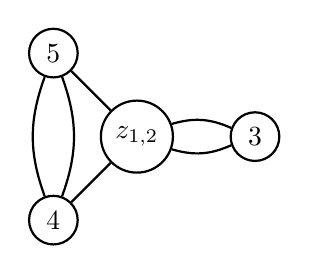
\begin{tikzpicture}[node distance={15mm}, thick, main/.style = {draw, circle}] 
            \node[main] (z) {$z_{1,2}$};
            \node[main] (3) [right of=z] {$3$};
            \node[main] (4) [below left of=z] {$4$};
            \node[main] (5) [above left of=z] {$5$}; 


            \draw (z) edge[bend right = 20] (3);
            \draw (z) edge[bend left = 20] (3);
            \draw (5) -- (z);
            \draw (4) -- (z);
            \draw (4) edge[bend right = 20] (5); 
            \draw (4) edge[bend left = 20] (5);
\end{tikzpicture}\newline\newline
Actually, the probability that at the first run Karger's algorithm returns a minimum cut is \textbf{not} high. The idea is to repeat the procedure $k$ times to reduce the probability of error. The value of $k$ will be determined by the analysis of the algorithm.\newpage
\begin{algorithm}
\caption{Karger's algorithm}\label{KARGER}
    \begin{algorithmic}[1]
    \Procedure{Karger($G, k$)}{}
        \State $min = \infty$
        \For{$i = 1$ to $k$}
            \State $t =$ \textit{FULL\_CONTRACTION($G$)}
            \If{$t < min$}
                \State $min = t$
            \EndIf
        \EndFor
        \Return $min$
    \EndProcedure   
    \end{algorithmic}
\end{algorithm}

\begin{algorithm}
\caption{FULL\_CONTRACTION}\label{FULLC}
    \begin{algorithmic}[1]
    \Procedure{FULL\_CONTRACTION($G = (V, E)$)}{}
        \For{$i = 1$ to $n - 2$}
            \State $e = $ random($E$)
            \State $G' = (V', E') = G_{/e} \quad \text{//Contraction}$
            \State $V = V'$
            \State $E = E'$
        \EndFor
        \Return $|E|$
    \EndProcedure   
    \end{algorithmic}
\end{algorithm}
\section{Analysis of Karger's algorithm}
We'll show for which value of $k$ the algorithm returns a minimum cut with high probability.\newline\newline
\textbf{Property:} $\forall$ cut $C'$ in $G_{/e}$ $\exists$ a cut $C$ in $G$ of the same cardinality.\newline\newline
This implies that $|\text{minimum cut in }G_{/e}| \geq |\text{minimum cut in } G|$.\newline\newline
\textbf{Proof:}Given a cut $C'$ in $G_{/e}$, the idea is to determine the corresponding cut $C$ in $G$ by substituting each edge $(z_{u, v}, y)$ in $C'$ with $(u, y)$ or $(v, y)$. Then, it remains to show that $C$ is a cut in $G$.\newline\newline
Let $C'$ be a cut in $G_{/e} = (V', E')$. Then, $C'$ separates $V'$ in 2 connected components. Let $V_1 \subset V'$ the connected component containing $z_{u,v}$, and let $x \notin V_1$. Then, in $G_{/e}$ every path from $z_{u, v}$ to $x$ must use an edge in $C'$.\newline\newline
Now we'll show that $C$ in $G$ disconnects $u$ and $v$ from $x$. Assume by contradiction that $C$ is \textbf{not} a cut in $G$. This implies that it exists a path between $u$ and $x$ after the removal of $C$ from $E$. Then, the path between $z_{u, v}$ and $x$ \textit{survives} the removal of $C'$ in $G_{/e}$. This implies that $C'$ is not a cut in $G_{/e} \rightarrow$ contradiction!\newline\newline
Note that the cuts that disappear in the contracted graph are the ones hit by the random choice of the edge $e$, all the others are preserved. This means that the only time the algorithm fails is when an edge belonging to a minimum cut in $G$ is hit by the random choice. Basically, by proving the property above we have shown that, if the algorithm never hits an edge belonging to a minimum cut, then it returns a correct solution (because the minimum cut is preserved in $G_{/e}$).\newline\newline
Therefore, we want the probability of \textbf{not} hitting edges of the minimum cut to be sufficiently high.

\subsection{Conditional probability recall}
\textbf{Definition:} The events $E_1, E_2$ are \textbf{independent} if:
\[P(E_1 \cap E_2) = P(E_1) \cdot P(E_2)\]
\textbf{Definition:} Given $P(E_1) > 0$, then:
\[P(E_2 | E_1) = \frac{P(E_1 \cap E_2)}{P(E_1)}\]
extension to $k$ events:
\[P(E_1 \cap E_2 \cap E_3 \cap ... \cap E_k) = P(E_1)P(E_2 | E_1)P(E_3 | E_1 \cap E_2) ... P(E_k | E_1 \cap ... \cap E_{k-1})\]

\subsection{Analysis of \textit{FULL\_CONTRACTION}}
\textbf{Intuition:} Since $|\text{min. cut}|$ is a small portion of $|E|$, it is \textit{unlikely} to hit an edge of a minimum cut. Let's calculate what is this probability.\newline\newline
\textbf{Property:} Let $G=(V, E), \,\, |V| = n$. If $G$ has a minimum cut of size $t$, then $|E| \geq t \cdot \frac{n}{2}$.\newline\newline
\textbf{Proof:} $d(v) \geq t \,\, \forall v \in V$. This is because If we take a node and remove all the edges incident to that node, that's a cut.
\[
    \begin{split}
        \sum_{v \in V}d(v) & = 2m \geq t \cdot n\\
        m & = |E| \geq \frac{t \cdot n}{2}
    \end{split}
\]
Let $t = |\text{minimum cut}|$. Given the event $E_i = \text{in the i-th contruction i did \textbf{not} hit an edge of the minimum cut}$, it follows that:
\[
    \begin{split}
        P(\overline{E}_1) & = \frac{t}{|E|} \leq \frac{t}{t \cdot \frac{n}{2}} = \frac{2}{n}\\
        P(\overline{E}_1) & \leq \frac{2}{n}\\
        P(E_1) & \geq 1 - \frac{2}{n}\\
    \end{split}
\]
Since after every contruction $|V'| = |V| - 1$, the following holds:
\[
    \begin{split}
        P(E_2 | E_1) & \geq 1 - \frac{t}{t \cdot \frac{(n - 1)}{2}} = 1 - \frac{2}{n - 1}\\
        & ... \\
        P(E_i | E_1 \cap ... \cap E_{i-1}) & \geq 1 - \frac{t}{\frac{t(n- i + 1)}{2}} = 1 - \frac{2}{n - i + 1}
    \end{split}
\]
Therefore, the probability that \textit{FULL\_CONTRUCTION} succeeds becomes:
\[
    \begin{split}
        P(\textit{FULL\_CONTRUCTION succeeds}) & \geq P(\bigcap_{i = 1}^{n-2}E_i) = \prod_{i = 1}^{n - 2}\left(1 - \frac{2}{n - i + 1}\right) = \prod_{i = 1}^{n-2} \frac{n - i -1}{n - i + 1}\\
        & \geq \frac{\cancel{n - 2}}{n} \cdot \frac{\cancel{n - 3}}{n - 1} \cdot \frac{\cancel{n - 4}}{\cancel{n - 2}} \cdot\cdot\cdot \frac{\cancel{3}}{\cancel{5}}\cdot\frac{2}{\cancel{4}}\cdot\frac{1}{\cancel{3}} = \frac{2}{n(n - 1)}
    \end{split}
\]
Basically, the probability that \textit{FULL\_CONTRUCTION} does not hit an edge of a minimum cut is at least $\frac{2}{n^2}$. Not so good as a bound. Our algorithm may err
in declaring the cut it outputs to be a min-cut. Karger's amplifies this probability by repeating \textit{FULL\_CONTRUCTION} multiple times:
\[P(\textit{the k runs of FULL\_CONTRUCTION do not return the minimum cut}) \leq \left(1 - \frac{2}{n^2}\right)^{k}\]
We want to find a value for $k$ such that $\left(1 - \frac{2}{n^2}\right)^{k} \leq \frac{1}{n^d}$. In order to do this, we'll use the following two rules:
\begin{itemize}
    \item $(1 + \frac{x}{y})^y \leq e^x \,\, y \geq 1, y \geq x$
    \item $e^{-ln\,n} = \frac{1}{n}$
\end{itemize}
By choosing $k = d\frac{n^2}{2}ln\,n$, it follows that:
\[
    \begin{split}
        & = \left(\left(1 - \frac{2}{n^2}\right)^{n^2}\right)^{\frac{d}{2}ln\, n}\\
        & \leq (e^{-2})^{\frac{d}{2}ln\, n} = e^{-ln\, n^d} = \frac{1}{n^d}
    \end{split}
\]
Then, by choosing that value for $k$ the Karger's algorithm succeeds with high probability:
\[P(\textit{Karger's succeeds}) \geq 1 - \frac{1}{n^d}\]

\subsection{Complexity}
\textit{FULL\_CONTRUCTION} can be implemented in $O(n^2)$. Then, the complexity of Karger's algorithm is $O(n^4log\, n)$. It is not very fast, but it can be improved to obtain a complexity of $O(n^2log^3\,n)$.\newline\newline
The fastest algorithm for this problem has a complexity of $O(m log\,n)$.

\chapter{Lec 21 - Autoencoders}

\section{Autoencoder - General Idea}
Autoencoders (AEs) are an unsupervised learning technique based on feed forward neural networks. The aim of autoencoders is to learn a representation (often called encoding or code) for a set of data, typically for the purpose of dimensionality reduction.\newline\newline
In particular, an autoencoder is a neural network that is trained to attempt to copy its input to its output.  Internally, it has a hidden layer $\textbf{h}$ that describes a code used to represent the input. The network may be viewed as consisting of two parts:
\begin{itemize}
    \item An \textbf{encoder} function $\textbf{h} = f(\textbf{x})$
    \item A \textbf{decoder} function that produces a reconstruction $\textbf{r} = g(\textbf{h})$
\end{itemize}
Since it is not useful to learn the identity function on the whole input domain (hidden code dimension equal to input dimension), autoencoders are trained to learn $\textbf{x} = g(f(\textbf{x}))$ with constraints:
\begin{itemize}
    \item on the architecture of the network (\textbf{undercomplete autoencoder}).

    \item adding a regularizing term to the loss (\textbf{overcomplete autoencoder})
\end{itemize}
Usually they are restricted in ways that allow them to copy only approximately. Because the model is forced to prioritize which aspects of the input should be copied, it often learns \textbf{useful properties} of the data.\newline\newline
Modern autoencoders have generalized the idea of an encoder and a decoder beyond deterministic functions to stochastic mappings $p_{encoder}(\textbf{h} | \textbf{x})$ and $p_{decoder}(\textbf{x} | \textbf{h})$. we may think of the decoder as providing a conditional distribution $p_{decoder}(\textbf{x} | \textbf{h})$. We may then train the autoencoder by minimizing $-log\, p_{decoder}(\textbf{x}|\textbf{h})$.

\section{Undercomplete Autoencoders}
One way to obtain useful features from the autoencoder is to constrain $\textbf{h}$ to have smaller dimension than $\textbf{x}$. An autoencoder whose code dimension is less than the input dimension is called \textbf{undercomplete}. Learning an undercomplete representation forces the autoencoder to capture the most salient features of the training data.\newline\newline
The learning process is described simply as minimizing a loss function;
\[L(\textbf{x}, g(f(\textbf{x}))\]
where $L$ is a loss function penalizing $g(f(\textbf{x}))$ for being dissimilar from $\textbf{x}$, such as the mean squared error.\newline\newline
When the decoder is linear and $L$ is the mean squared error, an undercomplete autoencoder learns to span the same subspace as \textbf{PCA} (SVD). Autoencoders with nonlinear encoder functions $f$ and nonlinear decoder functions $g$ can thus learn a more powerful nonlinear generalization of PCA. However, if the encoder and decoder are allowed too much capacity, the autoencoder can learn to perform the copying task without extracting useful information about the distribution of the data.\newline\newline
Autoencoders are often trained with only a single layer encoder and a single layer
decoder. However, this is not a requirement. In fact, using deep encoders and
decoders offers many advantages. Depth can exponentially reduce the computational cost of representing some functions. Depth can also exponentially decrease the amount of training data needed to learn some functions. Experimentally, \textbf{deep autoencoders} yield much better compression than corresponding shallow or linear autoencoders.

\subsection{Singular Value Decomposition (SVD)}
Singular Value Decomposition (SVD) is a standard linear dimensionality reduction method which combines the features of the original high-dimensional dataset and project them into a lower-dimensional space, ideally retaing most of their intrinsic properties.\newline\newline
Given a matrix $X$, the SVD decomposes it into the product of two unitary matrices, $V$ and $U$, and a rectangular diagonal matrix of singular values $S$:
\[X=V \cdot S \cdot U^T\]
The values in $S$ are called singular values. We can choose to keep only the first $k$ singular values in order to reduce the dimensionality of the input while minimizing the information loss.

\section{Overcomplete Autoencoders}
\textbf{Overcomplete} autoencoders have the hidden code dimension greater than the input. However, autoencoders may fail to learn useful properties of data if the dimension of the code $\textbf{h}$ is greater or equal to the input dimension. Therefore, rather than limiting the model capacity by keeping the encoder and decoder shallow and the code size small, \textbf{regularized autoencoders} use a loss function that encourages the model to have other properties besides the ability to copy its input to its output.\newline\newline
There are different types of regularized autoencoders:
\begin{itemize}
    \item Sparse autoencoders
    \item Denoising autoencoders 
    \item Contractive autoencoders
    \item Autoencoders with Dropout on the hidden layer
\end{itemize}

\section{Sparse Autoencoders}
A sparse autoencoder limits the capacity of the model by adding a sparsity penalty $\Omega(\textbf{h})$ on the code layer $\textbf{h}$, to the cost function:
\[L(\textbf{x}, g(f(\textbf{x}))) + \Omega(\textbf{h})\]
The sparsity penalty makes the model able to perform feature selection. In this way, a sparse autoencoder does not learn just the identity function, but it can learn useful features of the input.\newline\newline
Rather than thinking of the sparsity penalty as a regularizer for the copying task, we can think of the entire sparse autoencoder framework as approximating maximum likelihood training of a generative model that has latent variables (see slides for more details).

\section{Denoising Autoencoders}
Traditionally, autoencoders minimize some function:
\[L(\textbf{x}, g(f(\textbf{x})))\]
A \textbf{denoising autoencoder} or DAE instead minimizes:
\[L(\textbf{x}, g(f(\Tilde{\textbf{x}})))\]
where $\Tilde{\textbf{x}}$ is is a copy of $\textbf{x}$ that has been corrupted by some form of noise. Basically, DAE are forced to reconstruct a corrupted representation of the input. Denoising autoencoders must therefore undo this corruption rather than simply copying their input.\newline\newline
Like many other machine learning algorithms, autoencoders exploit the idea
that data concentrates around a low-dimensional \textbf{manifold}. Autoencoders aim to learn the structure of the manifold.
\begin{center}
    \includegraphics[scale=0.6]{images/manifold.png}
\end{center}

\section{Contractive Autoencoders}
The \textbf{contractive autoencoder} introduces an explicit regularizer on the code $\textbf{h} = f(\textbf{x})$, encouraging the derivatives of $f$ to be as small as possible:
\[\Omega(\textbf{h}) = \lambda ||\frac{\partial f(\textbf{x})}{\partial \textbf{x}}||^2_F\]
The penalty $\Omega(\textbf{h})$ is the squared Frobenius norm (sum of squared elements) of the Jacobian matrix of partial derivatives associated with the encoder function.\newline\newline
This forces the model to learn a function that does not change much when $\textbf{x}$ changes slightly.


\chapter{Lec 22 - Analysis of Randomized Quicksort}

\section{Randomized Quicksort}
\begin{algorithm}
\caption{Randomized Quicksort}\label{RQS}
    \begin{algorithmic}[1]
    \Procedure{RandQuicksort($S$)}{}
        \If{$|S| \leq 1$}
            \Return $S$
        \EndIf
        \State $p = \text{random($S$)}\quad \text{// pick a pivot element uniformly at random from $S$}$
        \State $S_1 = \{x \in S\,\, \text{s.t. }x < p\}$
        \State $S_2 = \{x \in S\,\, \text{s.t. } x > p\}$
        \State $z_1 = RandQuicksort(S_1)$
        \State $z_2 = RandQuicksort(S_2)$
        \State \Return $z_1, z_2$
    \EndProcedure   
    \end{algorithmic}
\end{algorithm}
It is a \textit{LAS VEGAS} algorithm (we choose the pivot at random).\newline\newline
Suppose that $p$ is always the median of $S$, then:
\[
    T_{RQS}(n) = 
    \begin{cases}
        2T_{RQS}(\frac{n}{2}) + O(n) & n > 1 \\
        0 & n\leq 1
    \end{cases}
\]
where $n = |S|$. Then $T_{RQS}(n) = O(nlog\,n)$.\newline\newline
However, $p$ is the median with probability $\frac{1}{n}$, very low. Actually, there exists a deterministic linear algorithm to compute the median. This implies that this version of deterministic Quicksort has complexity $O(nlog\,n)$. The problem is that the hidden constant is very high, thus it is inefficient in practice.\newline\newline
Fortunately, we don't really need that the random choice hits always the median. For example, let's see what happens if the pivot is always chosen between the $(\frac{n}{4} + 1)$-th order statistics and the $(\frac{3}{4}n)$-th order statistics. By looking at the recursion tree, if such a pivot is always chosen, all the root-leaf paths are no longer than $log_{\frac{4}{3}}n$. This is because $|S|$ after $i$ \textit{successes} is $\leq (\frac{3}{4})^in$. This implies that $T_{RQS} = O(nlog\,n)$. It is not necessary that $S_1$ and $S_2$ are perfectly balanced.\newline\newline
If we prove that the depth of the recursion tree is $O(log\,n)$ w.h.p. then $T_{RQS} = O(nlog\,n)$ w.h.p.

\section{Analysis}
Let's call the event $E = \textit{lucky choice of the pivot}$, that is, pivot chosen between the $(\frac{n}{4} + 1)$-th order statistics and the $(\frac{3}{4}n)$-th order statistics. Then:
\[P(E) = \left(\frac{\frac{3}{4} - (\frac{n}{4} + 1) + 1}{n}\right) = \frac{1}{2}\]
Fix \textbf{one} root-leaf path $P_1$:\newline\newline
\textbf{Lemma:} $P(|P_1| > a \cdot log_{\frac{4}{3}}n) < \frac{1}{n^3}$.\newline\newline
If this lemma is true, it follows that:
\begin{enumerate}
    \item Given the event $E_i = \textit{the path $p_i$ has length } > a \cdot log_{\frac{4}{3}}n$:
    \[P(\exists \textit{ a path with length } > a \cdot log_{\frac{4}{3}}n) = P\left(\bigcup_{i=1}^n E_i\right) \leq \sum_{i=1}^n P(E_i) < \frac{1}{n^2}\]

    \item Therefore, the probability that all the root-leaf paths have length $\leq a \cdot log_{\frac{4}{3}}n$ is the following:
    \[P(\textit{all the root-leaf paths have length $\leq a \cdot log_{\frac{4}{3}}n$}) \geq 1 - P(\exists \textit{ a path with length } > a \cdot log_{\frac{4}{3}}n) \geq 1 - \frac{1}{n^2}\]
\end{enumerate}
This would imply that $T_{RQS}(n) = O(nlog\,n)$ w.h.p.\newline\newline
It remains to prove the Lemma above.\newline\newline
\textbf{Proof:} Given a path $\Pi$, let $l = a \cdot log_{\frac{4}{3}}n$. We want to study the event $E =$ \textit{in the first l nodes of $\Pi$ there have been $< log_{\frac{4}{3}}n$ lucky choices}.
\begin{itemize}
    \item $X_i \quad 1 \leq i \leq l$
    \item $X_i = 1$ if at the $i$-th node of $\Pi$ there is a \textit{lucky choice} of the pivot. 
    \item $P(X_i = 1) = \frac{1}{2} \quad \forall i$.
    \item $X_i$ are independent.
\end{itemize}
We want the probability $P(\sum_{i=1}^l X_i) < log_{\frac{4}{3}}n$ to be bound.\newline\newline
Given $X = \sum_{i=1}^l X_i$, its expected value is defined as follows:
\[\mu = E[X] = E\left[\sum_{i=1}^l X_i\right] = \sum_{i=1}^l E[X_i] = \sum_{i=1}^l \frac{1}{2} = \frac{a}{2}log_{\frac{4}{3}}n\]
Now, let's apply the following Chernoff bound:
\[P(X < (1 - d)\mu) < e^{-\mu\frac{d^2}{2}} \quad 0 < d \leq 1\]
We want $(1 - d)\mu = log_{\frac{4}{3}}n$:
\[(1-d)\frac{a}{2}log_{\frac{4}{3}}n = log_{\frac{4}{3}}n\]
One possible solution is:
\begin{itemize}
    \item $a = 8$
    \item $d = \frac{3}{4}$
\end{itemize}
\[
    \begin{split}
        P(X < log_{\frac{4}{3}}n) & < e^{-\frac{8}{4}log_{\frac{4}{3}}n \cdot \frac{9}{16}} \\
        & = e^{-log_{\frac{4}{3}}n\cdot\frac{9}{8}}\\
        & < e^{-log_{\frac{4}{3}}n}\\
        & = e^{-\frac{ln\,n}{ln\,\frac{4}{3}}}\\
        & = \left(e^{-ln\,n}\right)^{\frac{1}{ln\,\frac{4}{3}}}\\
        & = \left(\frac{1}{n}\right)^{1/ln\,\frac{4}{3}}\\
        & < \frac{1}{n^3}
    \end{split}
\]


\end{document}
